
% load package if document contains at least one citation
\usepackage[maxbibnames=99,sorting=none,style=numeric,backend=biber]{biblatex}
% enable option to print bibliography as a numbered subsection
\defbibheading{bibsubsection}[\bibname]{%
  \subsection{#1}%
}
\addbibresource{refs.bib}

\begin{document}

\lstset{style=Python}
%% Project-specific Preambles 
\settoggle{includelogo}{true}

\newcommand{\thesubject}{Informatik}
\newcommand{\thetopic}{Netzwerke}
\newcommand{\thelogo}{Logos/FreeFlower}
\newcommand{\logosize}{.1\textwidth}

\lhead[ \leftmark ]{\thetopic}
\rhead[\thesubject]{\textcopyleft{} \href{https://github.com/CyrilBlum/FreeFlower}{FreeFlower}, \thetopic, \the\year}

\def\arrayB{"bar-chart","laptop","technologist","robot","woman-student","globe-with-meridians", "satellite", "satellite-antenna"}
\maketitlepage{\thetopic}{}
\tableofcontents\newpage

% content %%
\newtcolorbox{scaffoldBox}[1][]{
    enhanced jigsaw,
    breakable,
    parbox=false,
    attach boxed title to top text left={yshift=-3mm,yshifttext=-3mm},
    %  attach boxed title to top text left={yshift=-3mm},
    colback=\teacherColor!10,
    colframe=\teacherColor,
    colbacktitle=\teacherColor,
    #1}

\newtcolorbox{mainBox}[1][]{
    enhanced jigsaw,
    breakable,
    parbox=false,
    attach boxed title to top text left={yshift=-3mm,yshifttext=-3mm},
    %  attach boxed title to top text left={yshift=-3mm},
    colback=ForestGreen!10,
    colframe=ForestGreen,
    colbacktitle=ForestGreen,
    #1}


% Farben für jede Schicht
\newcommand{\applicationLayerColor}{Gold}
\newcommand{\transportLayerColor}{Indigo}
\newcommand{\networkLayerColor}{RoyalBlue}
\newcommand{\dataLinkLayerColor}{Gray}

% contents
% \chapter{Problemformulierung}

\begin{tcolorbox}[colback=blue!5!white, colframe=blue!80!black, title=Kontext]
    \begin{table}[H]
        \centering
        \renewcommand{\arraystretch}{1.2}
        \begin{tabular}{@{}r|p{0.65\linewidth}@{}}
            \textbf{Gymnasialstufe} & 2. Jahr Kurzzeitgymnasium (1. Semester)                                                                                   \\
            \midrule
            \textbf{Alter}          & 16–17 Jahre                                                                                                               \\
            \midrule
            \textbf{Vorwissen}      & Grundlegende Programmierkenntnisse in Python; Einführung in Netzwerke, IP-Adressen, Ports und Client-Server-Architekturen \\
        \end{tabular}
    \end{table}
\end{tcolorbox}

Die Lernenden begegnen täglich Formen digitaler Kommunikation – sei es über WhatsApp, Instagram oder Online-Games. Doch wie Nachrichten in Sekundenbruchteilen von einem Gerät zum anderen gelangen, bleibt für sie ein „Black Box“-Phänomen. Das Problem, an dem sie sich abarbeiten sollen, lautet daher:

\begin{quote}
    \textit{„Wie ist es möglich, dass ich in Echtzeit mit anderen über das Internet kommunizieren kann?“}
\end{quote}

\textbf{Gegenwartsbedeutung:} Jugendliche nutzen Chats, Videocalls oder Multiplayer-Spiele selbstverständlich, ohne die dahinterliegende Infrastruktur zu verstehen. Durch die Problematisierung entsteht ein Bezug zu ihrer unmittelbaren Lebenswelt und ein Bewusstsein für Abhängigkeiten von Netzinfrastrukturen.

\textbf{Zukunftsbedeutung:} Kenntnisse über Netzwerke sind nicht nur für Informatik-Studiengänge oder IT-Berufe relevant, sondern allgemein für eine reflektierte Teilhabe an der digitalen Gesellschaft: Wer versteht, wie Kommunikation technisch abläuft, kann auch Fragen von Datenschutz, Netzneutralität und digitaler Souveränität kompetenter einordnen.

\textbf{Exemplarische Bedeutung:} Am Beispiel einer Chat-Kommunikation werden grundlegende Konzepte der Informatik sichtbar: IP-Adressen, Ports und Client-Server-Strukturen lassen sich am „alltäglichen Problem“ einer Chat-Nachricht erschliessen und können auf andere digitale Dienste (E-Mail, Streaming, Online-Banking) übertragen werden.

Das formulierte Problem ermöglicht es den Lernenden, technische Funktionsprinzipien mit ihrer eigenen Lebenswelt zu verbinden und diese kritisch zu reflektieren. Damit entspricht es sowohl den Prinzipien problemorientierten Lernens als auch Klafkis Anspruch auf eine didaktische Analyse.\clearpage
\chapter{Netzwerke}

\section{Netzwerke und das Internet}
Bevor wir uns mit dem Internet als spezielles Netzwerk befassen, wollen wir allgemein nochmals auf Netzwerke eingehen. Im Alltag treffen Sie Netzwerke an unterschiedlichsten Orten an, zum Beispiel:
\begin{itemize}
	\item Transport-Netzwerke: Die Post, DHL, Planzer, etc.
	\item Soziale Netzwerke: TikTok, Youtube, Instagram, etc.
	\item Mobilitäts-Netzwerke: Das Strassennetz, SBB, Flixbus, etc.
	\item Shopping-Netzwerke: Aliexpress, Uber, etc.
	\item Computer-Netzwerke: \textbf{Das Internet}, Firmen-Netzwerke etc.
\end{itemize}

All diese Netzwerke können als Graphen visualisiert und veranschaulicht werden. Gemeinsam ist allen Netzwerken, dass die einzelnen Knoten ihren \enquote{Wert} (ihren Nutzen) erst durch die Verbindung mit anderen Knoten erhalten. Anders gesagt, mit den Worten des \enquote{Erfinders des \gls{WWW}}, Tim Berners-Lee:

\begin{quotation}
	The web is more a social creation than a technical one.
\end{quotation}

Häufig werden die Begriffe \enquote{Internet} und \enquote{Computer-Netze}, bzw. \enquote{Rechner-Netze} austauschbar verwendet. Dabei ist es jedoch wichtig zu verstehen, dass dies zwei unterschiedliche Konzepte sind: während dem mit dem \textit{Internet} ein höchst komplexes, den gesamten Globus umspannendes Netzwerk von Computern gemeint ist, können lediglich zwei miteinander verbundene Computer bereits ein Rechnernetz bilden. Das Internet wird häufig auch als \textit{Netz von (Rechner-)Netzen} bezeichnet. Es ist daher wichtig, dass wir uns zuerst mit einfacheren Rechnernetzen befassen, da diese die Grundbausteine für das Internet bilden.

\subsection{Geschichte des Internets}
Kommunikation war schon seit jeher ein zentrales Bedürfnis der Menschheit. Mit der Erfindung des Telefons, des Radios und später des Internets hat sich die Art und Weise, wie wir kommunizieren, jedoch grundlegend vereinfacht sowie verändert. Im Folgenden schauen wir kurz die wichtigsten Schritte an, die zur Erfindung des Internets geführt haben.

\subsubsection*{Die Anfänge: ARPANET und die 1960er Jahre}
Die Motivation für die Entwicklung des \gls{ARPANET} lag darin, ein robustes, dezentrales Kommunikationsnetzwerk zu schaffen, das auch im Falle von Ausfällen einzelner Knoten funktionsfähig bleibt. Insbesondere sollte das Netzwerk den Austausch von Informationen zwischen Universitäten und Forschungseinrichtungen ermöglichen und die Zusammenarbeit fördern. Ein weiterer wichtiger Beweggrund war die Suche nach einer Kommunikationsinfrastruktur, die im Kontext des Kalten Krieges auch militärischen Anforderungen an Ausfallsicherheit und Flexibilität genügte.Dieses Netzwerk sollte ursprünglich militärischen Zwecken dienen, fand jedoch schnell Anwendung in der akademischen und Forschungswelt.

\begin{itemize}
	\item 1969: Die erste Nachricht wird zwischen zwei Computern am \gls{ARPANET} übertragen.
	\item 1972: Die erste E-Mail wird verschickt.
	\item 1973: \gls{ARPANET} wird international, erste Verbindungen nach Norwegen und Grossbritannien.
\end{itemize}

\begin{figure}[H]
	\centering
	
\includegraphics[width=.7\textwidth]{Grundlagen_Info/07_Netzwerke/Figures/arpanet.png}
	\caption{Ausbreitung des \gls{ARPANET} von 1969 bis 1977 (Quelle: \href{http://www.fibel.org/linux/lfo-0.6.0/node457.html}{fibel.org})}
\end{figure}

\subsubsection*{Die Entwicklung von Protokollen: \texorpdfstring{\acrshort{TCP}/\acrshort{IP}}{TCP/IP}}
Ein entscheidender Schritt in der Geschichte des Internets war die Entwicklung von Kommunikationsprotokollen, die es verschiedenen Netzwerken ermöglichten, miteinander zu kommunizieren. Insbesondere das \gls{TCP}/\gls{IP}-Protokoll, das 1983 als Standard eingeführt wurde, bildete die Grundlage für das moderne Internet.

\begin{itemize}
	\item 1983: Umstellung des \gls{ARPANET} auf \gls{TCP}/\gls{IP}.
	\item 1980er: Entstehung weiterer Netzwerke (z.B. CSNET, BITNET) und deren Zusammenschluss.
\end{itemize}

Eine schematische Darstellung der Verbindung von verschiedenen Netzwerken über das \gls{TCP}/\gls{IP}-Protokoll ist in \cref{table:osi-layers} zu finden.

\subsubsection*{Das \acrshort{WWW} und die 1990er Jahre}
Die Erfindung des \gls{WWW} durch Tim Berners-Lee im Jahr 1990 revolutionierte die Nutzung des Internets. Kernstück des \gls{WWW} ist das Hypertext Transfer Protocol (\gls{HTTP}), das es ermöglicht, Webseiten zu erstellen und diese gegenseitig zu verlinken. Mit der Einführung von \gls{HTML} konnten Inhalte strukturiert und formatiert werden. Dies führte zu einer explosionsartigen Zunahme von Webseiten und Nutzern. Eine typische Webseite, wie wir sie heute kennen, ist über eine Web-Adresse, oder genauer gesagt \gls{URL} erreichbar, wie in folgendem Beispiel:

\begin{lstlisting}[language=HTML]
https://www.beispielseite.ch/unterseite.html
\end{lstlisting}

Eine \gls{URL} (Uniform Resource Locator) ist eine eindeutige Adresse, die auf eine Ressource (meistens eine Datei) im Internet verweist. Sie besteht aus mehreren Teilen, darunter das Protokoll (\texttt{http://} oder \texttt{https://}), der Domain-Name (\texttt{www.beispielseite.ch}) und der Pfad zur Datei (\texttt{/unterseite.html}).

Der Domain-Name steht für einen Computer im Internet, auf dem die Webseite gespeichert ist. Dieser Computer wird auch als \textbf{Webserver} bezeichnet.

Jede Webseite ist dabei als einfache Textdatei gespeichert, mit der Dateiendung \texttt{.html} (oder \texttt{.htm}). \gls{HTML} ist dabei eine Art Code-Sprache, die es ermöglicht, Text, Bilder und Links zu strukturieren. Eine einfache HTML-Datei könnte zum Beispiel so aussehen:

\begin{lstlisting}[language=HTML]
<!DOCTYPE html>
<html>
<head>
	<title>Beispielseite</title>
</head>
<body>
	<h1>Willkommen auf der Beispielseite</h1>
	<p>Dies ist ein einfacher Textabschnitt.</p>
	<a href="https://www.andereseite.ch/start.html">Andere Webseite</a>
</body>
\end{lstlisting}
Auf der vorletzten Zeile sehen Sie den Link zu einer anderen Webseite. Dieser Link ist ein sogenannter \textbf{Hyperlink}, der es ermöglicht, von einer Webseite zu einer anderen zu navigieren. Hyperlinks sind das Herzstück des \gls{WWW} und ermöglichen die Vernetzung von Informationen im Internet. Sie bestehen aus einem Text (der anklickbar ist) und einer \gls{URL}, die die Adresse der verlinkten Seite angibt. Ein Protokoll namens \gls{HTTP} regelt, wie diese Links angefragt und die entsprechenden Seiten übertragen werden.

Ein Browser kann den \gls{HTML}-Code benutzerfreundlich anzeigen und Verweise auf andere Webseiten als anklickbare Links anzeigen. Die Kombination von \gls{HTML}, \gls{HTTP} und der \gls{URL} ermöglichte es, Informationen auf einfache Weise zu teilen und zu durchsuchen.

Mit der Einführung von grafischen Webbrowsern wurde das Internet für die breite Öffentlichkeit zugänglich und erlebte einen massiven Popularitätsschub.

\begin{itemize}
	\item 1991: Das \gls{WWW} wird der Öffentlichkeit vorgestellt.
	\item 1993: Der erste grafische Webbrowser (Mosaic) erscheint.
	\item 1995: Kommerzielle Nutzung des Internets wird möglich, Gründung von Unternehmen wie Amazon und eBay.
\end{itemize}

\begin{figure}[H]
	\centering
	
\includegraphics[width=.5\textwidth]{Grundlagen_Info/07_Netzwerke/Figures/tim-berners-lee.jpg}
	\caption{Sir Tim Berners-Lee, der \enquote{Erfinder} des \acrlong{WWW}, 2014 (Quelle: \href{https://de.wikipedia.org/wiki/Tim_Berners-Lee}{Wikipedia})}
\end{figure}

\subsubsection*{Das Internet im 21. Jahrhundert}
Im 21. Jahrhundert hat das Internet weiterhin rasant an Bedeutung gewonnen. Mit der Verbreitung von schnellem Breitband-Internet, Smartphones und sozialen Medien ist das Internet zu einem unverzichtbaren Bestandteil des täglichen Lebens geworden.

Eine der wichtigsten Erfindungen, um das Internet jederzeit und überall verfügbar zu machen, war das \textbf{Mobile Internet}. Mit der Einführung von Smartphones und mobilen Datenverbindungen wurde es möglich, jederzeit auf das Internet zuzugreifen. Dies führte zu einer Explosion von mobilen Anwendungen und Diensten, die das Internet noch zugänglicher machten. Insbesondere die Einführung des iPhones durch die Firma Apple im Jahr 2007 und die damit verbundene Verbreitung von Smartphones haben das Internet revolutioniert. Heute sind Smartphones allgegenwärtig und ermöglichen den Zugriff auf das Internet von nahezu jedem Ort aus.

\begin{itemize}
	\item 2000er: Verbreitung von schnellem Breitband-Internet, Aufstieg von Google, Facebook, YouTube.
	\item 2007: Einführung des iPhones, Beginn der Smartphone-Revolution (siehe \href{https://www.youtube.com/watch?v=MnrJzXM7a6o}{Video der Produktvorstellung im Jahr 2007}).
	\item 2010er: Mobile Internetnutzung, Smartphones, \gls{IoT}.
	\item Heute: Künstliche Intelligenz, 5G, weltweite Vernetzung.
\end{itemize}

\begin{figure}[H]
	\centering
	
\includegraphics[width=.8\textwidth]{Grundlagen_Info/07_Netzwerke/Figures/internet_use_by_income_class.pdf}
	\caption{Entwicklung der weltweiten Internetnutzung nach Einkommensklasse (Quelle: \href{https://data.worldbank.org/indicator/IT.NET.USER.ZS}{Weltbank-Daten})}
	\label{fig:internet_use_by_income_class}
\end{figure}

Wie auf \cref{fig:internet_use_by_income_class} zu sehen ist, hat sich die Internetnutzung in den letzten Jahren stark erhöht. Insbesondere in einkommensstarken Ländern ist die Internetnutzung nahezu flächendeckend, während in einkommensschwachen Ländern noch grosse Unterschiede bestehen. Dies wird gut ersichtlich auf der Karte (siehe \cref{fig:internet_use_by_income_class_map}).

\begin{figure}[H]
	\centering
	
\includegraphics[width=.8\textwidth]{Grundlagen_Info/07_Netzwerke/Figures/internet_use_map_2024.pdf}
	\caption{Internetnutzung nach Land, 2024 (Quelle: \href{https://data.worldbank.org/indicator/IT.NET.USER.ZS}{Weltbank-Daten})}
	\label{fig:internet_use_by_income_class_map}
\end{figure}
\newpage
\section{\texorpdfstring{\acrshort{TCP} / \acrshort{IP} und das Schichtenmodell}{TCP / IP und das Schichtenmodell}}
\subsection{Schichtenmodell: Analogie}
Die Kommunikation über das Internet verläuft in unterschiedlichen Teilschritten. Man spricht von dem \textit{Schichtenmodell}. Als Analogie zum Schichtenmodell sei folgende Situation gegeben, in der die Chefs zweier unterschiedlicher Firmen miteinander kommunizieren wollen (siehe \cref{fig:schichtenmodellAnalogie}):
\begin{enumerate}
	\item Chef 1 (\faFemale, in Europa) möchte mit Chef 2 (\faMale, in Asien) sprechen.
	\item Dazu übermittelt Chef 1 dem Sekretariat Ihre Nachricht an Chef 2. Das Sekretariat schreibt die Nachricht nieder und übermittelt der lokalen Post den Brief an Chef 2.
	\item Die lokale Post kümmert sich nun um den Transport zur asiatischen Post, wo der Brief an das Sekretariat von Firma 2 übergeben und schlussendlich an Chef 2 gelangt.
\end{enumerate}

\begin{figure}[H]
	\centering
	\begin{tikzpicture}[
			auto,
			block/.style={
					minimum width=3cm,
					node distance=1.5cm,
					rectangle,
					fill=RoyalBlue!50,
					align=center,
					rounded corners
				}
		]


		% Define the nodes with FontAwesome icons
		\node[block] (chefs) {\faFemale\ Chef};
		\node[block, below=of chefs] (secretariat) {\faPhone\ Sekretariat};
		\node[block, below=of secretariat] (postman) {\faMale\ Post};


		% Define the nodes with FontAwesome icons

		\node[block, right=of postman] (postman2) {\faMale\ Post};
		\node[block, above=of postman2] (secretariat2) {\faPhone\ Sekretariat};
		\node[block, above=of secretariat2] (chefs2) {\faMale\ Chef};


		% Draw the dashed arrows
		\draw[<->, dashed, RoyalBlue!50, thick] (chefs) -- (chefs2);
		\draw[<->, dashed, RoyalBlue!50, thick] (secretariat) -- (secretariat2);
		\draw[<->, dashed, RoyalBlue!50, thick] (postman) -- (postman2);

		\draw[->, line width=1mm,ForestGreen!50] (chefs) -- node[left]{\faComments} (secretariat) ;
		\draw[->, line width=1mm,ForestGreen!50] (secretariat) -- node[left]{\faEnvelope} (postman) ;
		\draw[->, line width=1mm,ForestGreen!50, bend right] (postman.south) to node[midway,below]{\faBicycle\ \faMotorcycle\ \faCar\ \faShip\ \faPlane} (postman2.south) ;
		\draw[->, line width=1mm,ForestGreen!50] (postman2) -- node[right]{\faEnvelope} (secretariat2) ;
		\draw[->, line width=1mm,ForestGreen!50] (secretariat2) -- node[right]{\faComments} (chefs2) ;

		% fit rectangles around regions
		\node[fit=(chefs) (postman), inner sep=8pt, red, dotted, draw, line width=1pt,rounded corners](region1) {};
		\node[fit=(chefs2) (postman2), inner sep=8pt, red, dotted, draw, line width=1pt,rounded corners](region2) {};
		% annotate both rectangles
		\node[above=5pt of region1.north, anchor=center, align=center]{\textcolor{red}{Firma 1, Europa}};
		\node[above=5pt of region2.north, anchor=center, align=center]{\textcolor{red}{Firma 2, Asien}};

	\end{tikzpicture}
	\label{fig:schichtenmodellAnalogie}
	\caption{Analogie zum Schichtenmodell: Kommunikation zwischen zwei grossen Firmen}
\end{figure}

Dieser Kommunikationsablauf kann in Schichten mit jeweiligen dazugehörigen Prozessen aufgeteilt werden:
\begin{enumerate}
	\item \textbf{Schicht \enquote{Chefs}}: damit die beiden Chefs mit einander sinnvolle Gespräche führen können, verfügen Sie über gemeinsame Standards (Sprache, Wissen etc.) sowie Protokolle (standardisierte Abläufe der Begrüssung etc.).
	\item \textbf{Schicht \enquote{Sekretariat}}: Damit die Sekretariate miteinander kommunizieren können, benötigen auch sie standardisierte Abläufe oder Protokolle, etwa, wie man einen Brief korrekt verfasst, datiert und adressiert.
	\item \textbf{Schicht \enquote{Post}}: Die Post verfügt ebenfalls über standardisierte Protokolle (wie werden Briefe und Pakete von A nach B transportiert? Mit welchen Transportmitteln, über welche Routen?)
\end{enumerate}
Die Vorteile des Schichtenmodells scheinen offensichtlich:
\begin{itemize}
	\item \textbf{Unabhängigkeit der Schichten}: Falls die Post das Transportmittel ändert, müssen die Sekretariate die Briefe nicht neu verfassen.
	\item \textbf{Modularität und Spezialisierung}: Statt das jemand alles tun muss (Chef 1 reist nach Asien zu Chef 2), kann der Prozess für die jeweiligten Beteiligten schnell und effizient abgewickelt werden.
\end{itemize}

\subsection{\texorpdfstring{Schichtenmodelle \acrshort{TCP} / \acrshort{IP} und \acrshort{OSI}}{TCP / IP und OSI}}

Im Zusammenhang mit dem Internet werden häufig zwei Schichtenmodelle gegenübergestellt: Das vollständige, detaillierte \acrfull{OSI}-Modell mit 7 Schichten sowie das etwas vereinfachte \acrfull{TCP}-\acrfull{IP}-Modell mit 4 Schichten. Die beiden Schichten, deren Aufgaben, Informationsformen und Protokolle sind in \cref{table:osi-layers} abgebildet.


\begin{table}[H]
	\centering
	\footnotesize
	\input{Grundlagen_Info/07_Netzwerke/Skript/Includes/chapter01_osi-tcpip-table.tex}
	\label{table:osi-layers}
	\caption{Internet-Schichten-Modelle \gls{OSI} und \gls{TCP}-\gls{IP} sowie deren wichtigste Aufgaben, Informationsformen, Geräte und Protokolle}
\end{table}

\begin{myexercise}[Netzwerkspiel]\label{ex:schichtenmodell-spiel}
	Verwenden Sie die Vorlage aus \ref{chapter:netzwerkspiel}, um in der Klasse Nachrichten auszutauschen. Notieren Sie sich dabei:
	\begin{itemize}
		\item Welche Schicht für welche Aufgabe zuständig ist.
		\item Welche Protokolle und Geräte in den jeweiligen Schichten verwendet würden.
	\end{itemize}
	\begin{myanswer}
		\begin{itemize}
			\item \gls{IP}-Adresse: Vermittlungsschicht / Internet-Schicht
			\item Sequenz-Nummer: Transportschicht
			\item Nachricht: Anwendungsschicht
			\item Protokolle (Analog zum Spiel):
			      \begin{itemize}
				      \item \gls{HTTP}: Anwendungsschicht
				      \item \gls{TCP}: Transportschicht
				      \item \gls{IP}: Vermittlungsschicht
			      \end{itemize}
		\end{itemize}
	\end{myanswer}
\end{myexercise}

Im Folgenden gehen verwenden wir hauptsächlich das etwas vereinfachte \acrfull{TCP}-\acrfull{IP}-Modell und gehen kurz auf jede Schicht ein.

Im echten Internet werden Daten häufig als \textbf{Frame} (Paket) verschickt, ähnlich wie im Spiel aus \cref{ex:schichtenmodell-spiel}. Jedes Paket besteht dabei aus einem \textbf{Header} (Kopfteil) und einem \textbf{Payload} (Nutzteil). Der Header enthält dabei wichtige Informationen über das Paket, wie zum Beispiel die Quell- und Zieladresse, die Sequenznummer und andere Metadaten. Der Payload enthält die eigentlichen Daten, die übertragen werden sollen (z.B. eine Nachricht, ein Bild, ein Video etc.). Jede Schicht fügt dabei ihren eigenen Header hinzu, bevor das Paket an die nächste Schicht weitergegeben wird. Beim Empfänger werden die Header in umgekehrter Reihenfolge entfernt, um die ursprünglichen Daten wiederherzustellen.

\begin{figure}[H]
	\centering
	\input{Grundlagen_Info/07_Netzwerke/Skript/Includes/chapter01_fig_schichtenmodell.tex}
	\caption{Illustration eines Datenpakets durch die verschiedenen Schichten des \gls{TCP}/\gls{IP}-Modells}
\end{figure}


\subsection{Begriffe: Client, Server und Host}
Bevor wir uns näher mit den Dimensionen der einzelnen Schichten befassen, sollten wir zuerst einige häufig auftauchende Begriffe klären, von denen im Kontext von Rechner-Netzen häufig die Rede ist.

\begin{mydefinition}[Client, Server und Host]\label{def:client-server-host}
Je nach Rolle der Computer in einem Rechner-Netz ist häufig von \textbf{Client}, \textbf{Server} oder \textbf{Host} die Rede.
\begin{itemize}
	\item Der \textbf{Client} $\mathcal{C}$ (von en. \textit{client} = \enquote{Kunde}) bezeichnet den Computer $\mathcal{C}$, der etwas von einem anderen Computer $\mathcal{S}$ will. Genauer gesagt handelt es sich nicht um den Computer selber, sondern um ein Programm auf einem Computer $\mathcal{C}$, das etwas anfordert von einem anderen Programm, das auf einem anderen Computer $\mathcal{S}$ läuft. Zur Vereinfachung sprechen wir jedoch häufig einfach von einem Computer $\mathcal{C}$ und einem Computer $\mathcal{S}$.
	\item Der \textbf{Server} $\mathcal{S}$ (von en. \textit{to serve} = \enquote{dienen}) bezeichnet  den Computer $\mathcal{S}$ (genauer gesagt das Computer-Programm $\mathcal{S}$), das dem Computer $\mathcal{C}$ gibt, was er will. Der Server kann Verbindungsanfragen von anderen Computern akzeptieren oder ablehnen.
	\item Bei einem \textbf{Host} (von englisch \textit{host} = \enquote{Wirt} / \enquote{Gastgeber}) ist im allgemeinen ein Computer in einem Netzwerk gemeint, der je nach Situation die Rolle des Servers oder Clients einnehmen kann. Der Name eines Computers in einem Netzwerk wird häufig als \textbf{Host Name} bezeichnet.
\end{itemize}
\end{mydefinition}


\section{\texorpdfstring{\textcolor{\dataLinkLayerColor}{Netzzugriff-Schicht}}{Netzzugriff-Schicht}}

\subsection{MAC-Adressen}
Bisher haben wir mehrheitlich darüber gesprochen, wie Datenpakete zwischen adressierten Empfängern (siehe \gls{IP}-Adressen) hin- und hergeschickt werden, und wie Adressen in (Sub-)Netzwerke unterteilt und in verständliche Namen umgewandelt werden können. Eine \gls{IP}-Adresse kann mit der Adresse eines Hauses verglichen werden. Allerdings legt der Briefträger die Briefe und Pakete nicht an einer Adresse ab, sondern in einem Briefkasten, also einem konkreten Objekt. Falls sich der Briefkasten oder sogar das ganze Haus ändert, so bleibt die Adresse doch dieselbe. Ähnlich dieser Analogie kann in einem Computer die gesamte Hardware ausgetauscht werden, inklusive der Netzwerkkarte, welche sich um das Verschicken und Empfangen von Daten kümmert, und trotzdem sollte der Datentransport zum Computer weiterhin funktionieren. Damit dies klappt, benötigen wir ein weiteres Protokoll, welches die \gls{IP}-Adresse in eine so genannte \gls{MAC}-Adresse umwandelt.

\begin{mydefinition}[\gls{MAC}-Adresse]
Die \gls{MAC}-Adresse ist die physische Adresse der Netzwerkkarte in einem Computer, also sozusagen der \enquote{Fingerabdruck} der Netzwerkkarte. Sie wird normalerweise mit 48 bit (= 6 Bytes) angegeben, welche normalerweise der Kürze wegen in hexadezimaler Schreibweise notiert werden. Ein Beispiel einer \gls{MAC}-Adresse könnte wie folgt aussehen: \commandbox{48-2C-6A-1E-59-3D}.
\end{mydefinition}

\subsection{\texorpdfstring{\gls{ARP}}{ARP}}
Damit ein Gerät innerhalb eines lokalen Netzwerks eine Nachricht an ein anderes Gerät senden kann, muss die \gls{IP}-Adresse des Empfängers in eine \gls{MAC}-Adresse umgewandelt werden. Da es jedoch keine direkte Möglichkeit gibt, eine \gls{MAC}-Adresse aus einer \gls{IP}-Adresse zu berechnen, muss ein spezielles Protokoll verwendet werden, um diese Zuordnung herzustellen. Dieses Protokoll wird als \textbf{Address Resolution Protocol} (\gls{ARP})  (auf Deutsch: \textit{Adressauflösungsprotokoll})  bezeichnet. Dieses wird jedes Mal ausgeführt, wenn ein Computer eine Nachricht an eine bestimmte \gls{IP}-Adresse senden will, aber die \gls{MAC}-Adresse des nächsten Empfängers (\textit{gateway})  noch  \textit{nicht} kennt. In diesem Fall sendet der Computer eine Anfrage an alle Computer im selben Subnetz (\textit{Broadcast}), um die \gls{MAC}-Adresse des gewünschten Empfängers zu erfahren. Der Computer mit der gesuchten \gls{IP}-Adresse antwortet dann mit seiner \gls{MAC}-Adresse (\textit{Unicast}) und der sendende Computer kann nun die Nachricht an den Empfänger weiterleiten.

Ein Beispiel, wie das \gls{ARP}-Protokoll funktioniert, könnte wie folgt aussehen:
\begin{itemize}
	\item Computer \commandbox|192.168.0.33| will Nachricht senden an \commandbox|192.168.0.34| im selben Subnetz (Subnetz-Maske: \commandBluebox|255.255.255.0|)
	\item \commandbox|192.168.0.33| sendet daher eine Nachricht an alle Computer in \commandbox|192.168.0.x|: \enquote{Wer hat die IP \commandbox|192.168.0.34|}?
	\item Computer \commandbox|192.168.0.34| antwortet: \enquote{Ich! Meine MAC ist \commandbox|60:4E:46:F5:08:09|.}
	\item Nun kann der Computer seine Nachricht direkt an den nächsten Empfänger (\textit{gateway}) übergeben.
\end{itemize}

Die Resultate aller \gls{ARP}-Anfragen werden in einer so genannten \textbf{ARP-Tabelle} gespeichert, damit nicht jedes Mal eine neue Anfrage gesendet werden muss. Diese Tabelle wird periodisch aktualisiert, um sicherzustellen, dass die Zuordnungen aktuell bleiben. Um die \gls{ARP}-Tabelle auf einem Computer anzuzeigen, kann der Befehl \commandbox*|arp -a| im Terminal (MacOS, UNIX-Systeme), bzw. \texttt{cmd} (Windows) verwendet werden.

\subsection{Ping}
% TODO potentially add tcolorbox for each terminal command introduced, with example use
Mit dem Befehl \commandbox*|ping| kann überprüft werden, ob ein Rechner im Netzwerk erreichbar ist. Dabei wird eine minimale, inhaltslose Nachricht an einen anderen Rechner (=\gls{IP}-Adresse) geschickt. Das Ziel ist es, zu überprüfen, ob eine gewisse \gls{IP}-Adresse im Netzwerk existiert. Der Befehl \enquote{\textit{ping}} ist vergleichbar mit einem Ping-Pong-Spiel: Der Absender-Rechner, der eine \enquote{ping}-Nachricht schickt, erhält vom Ziel-Rechner, sofern dieser erreicht wird, viermal eine \enquote{pong}-Nachricht zurückgeschickt. Der \texttt{ping}-Befehl kann im Terminal (MacOS, UNIX-Systeme), bzw \texttt{cmd} (Windows) wie folgt ausgeführt werden: \commandbox*|ping [ip address]|, also z.B. \commandbox*|ping 159.233.1.22|. Der Ping-Befehl verwendet das \gls{ICMP}-Protokoll (Internet Control Message Protocol) der Internetschicht, um die Nachrichten zu verschicken. Das \gls{ICMP}-Protokoll ist ein Protokoll, das speziell für die Übertragung von Kontroll-Nachrichten im Netzwerk entwickelt wurde, allerdings nicht für den Datentransfer von Nutzdaten.

\begin{mycaution}[Ping of Death]
	Eine Spezial-Variante des \texttt{ping}-Befehls ist der sogenannte \textcolor{red}{\faSkull{} Ping of Death}, bei dem ein bösartiger Computer ein zu grosses Datenpaket an einen anderen Computer schickte, das beim Zusammensetzen zum Zusammensturz des Zielrechners führte. Dies ist seit Ende der 90er-Jahre auf den meisten Computern nicht mehr möglich: Die Sicherheitslücke wurde behoben, indem beispielsweise die Paketgrösse vor dem Zusammensetzen überprüft wurde.
\end{mycaution}

\begin{myexercise}[Filius: Installation]
	Installieren Sie das Programm Filius, welches wir zur Modellierung von Netzwerken verwenden werden. Die Anleitung dazu finden Sie in \cref{subsec:filius-installation}.
\end{myexercise}

\begin{myexercise}[Filius-Anwendung: \acrshort{ARP} beobachten]
	Schauen Sie sich das \href{https://www.youtube.com/watch?v=Kn8v_HrckUM&list=PLUfZiVdJui-57k0VcRecHX0JTEhOMgiKP}{Filius-Video Nummer 1} an und führen Sie alle gezeigten Schritte ebenfalls in Filius aus.
\end{myexercise}

Ähnlich wie das Datenaustausch-Tool in Filius kann der Datenaustausch in einem echten Netzwerk mit einem Netzwerk-Analyse-Tool wie beispielsweise \textbf{WireShark} beobachtet werden. WireShark ermöglicht es, den gesamten Datenverkehr in einem Netzwerk mitzuschneiden und zu analysieren. So können auch die \gls{ARP}-Anfragen und -Antworten beobachtet werden.

\begin{myexercise}[WireShark-Auszug]
	Sie erhalten folgenden WireShark-Auszug eines \gls{ARP}-Protokolls. Beantworten Sie die Fragen dazu.
	\begin{figure}[H]
		\centering
		
\includegraphics[width=\textwidth]{Grundlagen_Info/07_Netzwerke/Figures/wiresharkARP.png}
		\caption{WireShark-Auszug eines \gls{ARP}-Protokolls}
		\label{fig:arp-wireshark}
	\end{figure}
	\begin{itemize}
		\item Welche \gls{IP}-Adresse hat der Computer, der die Anfrage sendet?
		\item Welche \gls{MAC}-Adresse hat der Computer, der die Anfrage sendet?
		\item Welche \gls{IP}-Adresse wird in der Anfrage gesucht?
		\item Welche \gls{MAC}-Adresse hat der Computer, der die Antwort sendet?
	\end{itemize}
	\begin{myanswer}
		\begin{itemize}
			\item \gls{IP}-Adresse des Computers, der die Anfrage sendet: \commandbox|172.20.10.5|
			\item \gls{MAC}-Adresse des Computers, der die Anfrage sendet: \commandbox|c6:ac:18:ce:15:45|
			\item \gls{IP}-Adresse des gesuchten Computers: \commandbox|172.20.10.1|
			\item \gls{MAC}-Adresse des gesuchten Computers: \commandbox|56:eb:e9:30:25:64|
		\end{itemize}
	\end{myanswer}
\end{myexercise}

\begin{mychallenge}[WireShark-Installation und \gls{ARP} mit WireShark beobachten]
	Installieren Sie das Netzwerk-Analyse-Tool \textbf{WireShark} auf Ihrem Computer (Anleitung siehe \href{https://www.wireshark.org/download.html}{wireshark.org}). Versuchen Sie, einen \gls{ARP}-Austausch in Ihrem eigenen Netzwerk zu beobachten. Dazu müssen Sie zuerst den \gls{ARP}-Cache Ihres Computers leeren. Folgende Befehle müssen in der Befehlszeile eingegeben werden, diese kann wie folgt geöffnet werden:

	\begin{itemize}
		\item Windows: Öffnen Sie die Eingabeaufforderung (cmd) via \keys{\faWindows+R} und Eingabe von \texttt{cmd}
		\item MacOS: Öffnen Sie das Terminal (z.B. über Spotlight-Suche)
	\end{itemize}

	Geben Sie danach folgenden Befehl zum Leeren des \gls{ARP}-Caches ein:
	\begin{itemize}
		\item Windows: \commandbox*|arp -d|
		\item MacOS: \commandbox*|sudo arp -a -d|
	\end{itemize}

	Danach müssen Sie in WireShark die richtige Netzwerkschnittstelle auswählen (z.B. WLAN oder Ethernet) und einen Display-Filter für \gls{ARP} setzen. Geben Sie dazu in das Filter-Feld Folgendes ein:

	\commandbox|arp && (arp.src.proto_ipv4 == MEINEIP or arp.dst.proto_ipv4 == MEINEIP)|

	Ihre \gls{IP}-Adresse können Sie mit dem folgenden Befehl in der Befehlszeile herausfinden:

	\begin{itemize}
		\item Windows: \commandbox*|ipconfig|
		\item MacOS: \commandbox*|ifconfig getifaddr en0|
	\end{itemize}

	Starten Sie die Aufnahme in WireShark und versuchen Sie, eine beliebige Webseite in Ihrem Browser zu öffnen. Beobachten Sie die \gls{ARP}-Anfragen und -Antworten in WireShark.
\end{mychallenge}

\subsection{Verschlüsselung von Netzwerken}
In einem lokalen Netzwerk können Datenpakete von jedem Gerät im selben Netzwerk abgefangen und gelesen werden. Um die Sicherheit und Vertraulichkeit der Daten zu gewährleisten, werden verschiedene Verschlüsselungsmethoden verwendet. Eine gängige Methode ist die Verwendung des \gls{WPA}-Protokolls, welches eine starke Verschlüsselung der Datenpakete ermöglicht. \gls{WPA} verwendet den \gls{AES}-Verschlüsselungsalgorithmus, um die Daten zu schützen. Dabei handelt es sich um einen symmetrischen Verschlüsselungsalgorithmus, welcher als sehr sicher gilt und in vielen Anwendungen eingesetzt wird.

Es gibt verschiedene Versionen von \gls{WPA}, darunter \gls{WPA}2 und \gls{WPA}3, die jeweils verbesserte Sicherheitsfunktionen bieten. In einem passwortfreien Netzwerk (offenes Netzwerk) sind die Datenpakete grundsätzlich unverschlüsselt und können von jedem Gerät im selben Netzwerk abgefangen und gelesen werden. Um dies zu illustrieren, schauen wir uns folgenden Wireshark-Auszug eines unverschlüsselten \gls{HTTP}-Datenpakets an.

\begin{myexample}[Wireshark-Auszug eines unverschlüsselten \gls{HTTP}-Datenpakets]
In \cref{fig:http-wireshark} ist ein Wireshark-Auszug eines unverschlüsselten \gls{HTTP}-Datenpakets zu sehen.
\begin{figure}[H]
	\centering
	
\includegraphics[width=\textwidth]{Grundlagen_Info/07_Netzwerke/Figures/exampleComWireshark}
	\caption{Wireshark-Screenshot während eines Webseitenaufrufs}
	\label{fig:http-wireshark}
\end{figure}
Im unteren Teil von \cref{fig:http-wireshark} ist der Payload des Pakets dargestellt, welcher den eigentlichen Inhalt der Nachricht enthält. In diesem Fall handelt es sich um eine \gls{HTTP}-Anfrage, die von einem Client an einen Server gesendet wird. Der Payload enthält dabei Informationen wie die angeforderte Ressource (z.B. eine Webseite), den Hostnamen des Servers und andere Metadaten. Da das Netzwerk unverschlüsselt ist, kann jeder, der Zugriff auf das Netzwerk hat, den Inhalt dieses Pakets lesen und somit die angeforderten Informationen einsehen.
\end{myexample}

\begin{mycaution}[Strafrechtliche Aspekte beim Mithören von Netzwerken]
	Das Abfangen und Mitlesen von Datenpaketen in einem Netzwerk ohne ausdrückliche Erlaubnis der beteiligten Parteien ist in vielen Ländern illegal und kann strafrechtlich verfolgt werden. In der Schweiz beispielsweise verstösst das unbefugte Abfangen von Daten gegen das Bundesgesetz über den Datenschutz (DSG) und das Strafgesetzbuch (StGB). Personen, die beim unbefugten Abfangen von Daten erwischt werden, können mit Geldstrafen oder sogar Freiheitsstrafen belegt werden. Es ist daher wichtig, die rechtlichen Rahmenbedingungen zu kennen und einzuhalten.
\end{mycaution}

\begin{myexercise}[WireShark-Auszug]
	Sam und Martina haben ein Python-Game geschrieben mit Multiplayer-Funktionalität innerhalb des lokalen Netzwerks. Sam hat das Spiel auf seinem Computer gestartet und Martina möchte sich mit Sams Spiel verbinden. Sams Computer hat die \gls{IP}-Adresse \commandbox|192.168.0.97| und Martinas Computer die \gls{IP}-Adresse \commandbox|192.168.0.121|. Unten ist ein WireShark-Auszug von Martinas Computer zu sehen, als sie versucht, sich mit Sams Spiel zu verbinden. Beantworten Sie die Fragen dazu.
	\begin{figure}[H]
		\centering
		
\includegraphics[width=\textwidth]{Grundlagen_Info/07_Netzwerke/Figures/wiresharkGame.png}
		\caption{WireShark-Auszug von Martinas Computer}
		\label{fig:game-wireshark}
	\end{figure}
	\begin{itemize}
		\item Über welches Protokoll versucht Martina, sich mit Sams Spiel zu verbinden? Welche Vorteile bietet dies gegenüber anderen möglichen Protokollen?
		\item Verwenden Sam und Martina ein unverschlüsseltes oder verschlüsseltes Netzwerk?
	\end{itemize}

	\begin{myanswer}
		\begin{itemize}
			\item Martina versucht, sich über das \gls{TCP}-Protokoll mit Sams Spiel zu verbinden. \gls{TCP} bietet den Vorteil, dass es eine zuverlässige, verbindungsorientierte Kommunikation ermöglicht. Es stellt sicher, dass alle Datenpakete in der richtigen Reihenfolge und ohne Verluste ankommen, was besonders wichtig für Multiplayer-Spiele ist, bei denen die Konsistenz der Spielzustände gewährleistet sein muss. Im Gegensatz dazu bietet beispielsweise \gls{UDP} keine Garantie für die Zustellung oder Reihenfolge der Pakete, was zu Inkonsistenzen im Spiel führen könnte. Trotzdem wird \gls{UDP} in einigen Spielen verwendet, da es schneller ist und weniger Overhead hat.
			\item Sam und Martina verwenden ein unverschlüsseltes Netzwerk, da die Daten im Payload lesbar sind.
		\end{itemize}
	\end{myanswer}

\end{myexercise}


\subsection{Switches}
Jede Netzwerkkarte kann nur mit genau einem anderen Gerät in einem lokalen Netzwerk kommunizieren. Damit mehrere Geräte in einem lokalen Netzwerk miteinander kommunizieren können, werden sogenannte \textbf{Switches} verwendet. Ein Switch ist ein Gerät, das mehrere Netzwerkkarten miteinander verbindet und es ihnen ermöglicht, Datenpakete direkt aneinander zu senden. Der Switch lernt dabei die \gls{MAC}-Adressen der angeschlossenen Geräte und leitet die Datenpakete nur an das Gerät weiter, für das sie bestimmt sind. Dadurch wird der Datenverkehr im Netzwerk effizienter gestaltet, da nicht alle Geräte jedes Datenpaket empfangen müssen.

\begin{myexercise}[Filius-Anwendung: Switch beobachten]
	Schauen Sie sich das \href{https://www.youtube.com/watch?v=Kn8v_HrckUM&list=PLUfZiVdJui-57k0VcRecHX0JTEhOMgiKP}{Filius-Video Nummer 2} an und führen Sie alle gezeigten Schritte ebenfalls in Filius aus.
\end{myexercise}

\subsection{Topologie}
Beim Erstellen eines Netzwerks stellt sich als Erstes die Frage, welche Computer man mit welchen anderen Computern verbinden soll. Die Struktur der Verbindungen in einem Netzwerk kann also umformuliert werden als Graphen-Problem, bei dem es zu bestimmen gibt, welche Knoten eines Graphen miteinander über eine Kante verbunden werden. In den folgenden Graphen bezeichnen Knoten die Computer und Kanten die Verbindungen (Kabel) zwischen den Computern. Die verschiedenen möglichen Strukturen eines Netzwerks werden auch als \textbf{Topologie} bezeichnet. Einige Beispiel-Topologien sind in \cref{fig:topologie} gezeigt.
\input{Grundlagen_Info/07_Netzwerke/Skript/Includes/chapter01_fig_topologies.tex}

Da Computer in Realität häufig nur über eine einzige Netzwerkkarte verfügen, können sie auch nur mit einem weiteren Computer verbunden werden. In einem lokalen Netzwerk (\gls{LAN}) trifft man daher häufig die Form einer Stern-Topologie an, bei der alle Computer mit einer zentralen \textbf{Switch} verbunden werden, also einem Gerät, welches mehrere Rechner an einem zentralen Punkt miteinander verbindet.

\begin{myexercise}[Topologien vergleichen]
	Vergleichen Sie die Stern-Topologie mit der Vollvermascht-Topologie:
	\begin{itemize}
		\item In welcher Topologie ist es einfacher, ein neues Gerät anzuschliessen?
		\item In welcher Topologie funktioniert die Kommunikation immer noch gut, selbst wenn einzelne Kabel oder Geräte ausfallen?
		\item In welcher Topologie müssen mehr Kabel gekauft werden?
	\end{itemize}
	\begin{myanswer}
		\begin{itemize}
			\item In der Stern-Topologie ist es einfacher, ein neues Gerät anzuschliessen, da nur ein Kabel zum zentralen Switch benötigt wird. Falls kein zentraler Switch benötigt wird, ist beispielsweise die vollvermaschte Topologie einfacher, da das neue Gerät zu jedem anderen Gerät maximal ein Kabel benötigt.
			\item In der Vollvermaschten Topologie funktioniert die Kommunikation immer noch gut, selbst wenn einzelne Kabel oder Geräte ausfallen.
			\item In der Vollvermaschten Topologie müssen mehr Kabel gekauft werden.
		\end{itemize}
	\end{myanswer}
\end{myexercise}

\begin{myexercise}[Kabelanzahl in Stern-Topologien]
	Wie viele Kabel müssen in der Stern-Topologie gekauft werden\dots
	\begin{itemize}
		\item Für 6 Geräte?
		\item Für 10 Geräte?
		\item Allgemeine Formel?
	\end{itemize}
	\begin{myanswer}
		\begin{itemize}
			\item Für 6 Geräte: 5 Kabel
			\item Für 10 Geräte: 9 Kabel
			\item Allgemeine Formel: $n-1$ Kabel, wobei $n$ die Anzahl der Geräte ist.
		\end{itemize}
	\end{myanswer}
\end{myexercise}

\begin{myexercise}[Kabelanzahl in Vollvermascht-Topologien]
	Wie viele Kabel müssen in der Vollvermascht-Topologie gekauft werden\dots
	\begin{itemize}
		\item Für 6 Geräte?
		\item Für 10 Geräte?
		\item Allgemeine Formel?
	\end{itemize}
	\begin{myanswer}
		\begin{itemize}
			\item Für 6 Geräte: 15 Kabel
			\item Für 10 Geräte: 45 Kabel
			\item Allgemeine Formel: $\frac{n(n-1)}{2}$ Kabel, wobei $n$ die Anzahl der Geräte ist.
		\end{itemize}
	\end{myanswer}
\end{myexercise}

\subsection{Unicast, Multicast und Broadcast}
Je nachdem für wie viele Teilnehmer eines Netzwerks eine Sendung bestimmt ist, unterscheidet man bei der Datenübertragung zwischen \textbf{Unicast}, \textbf{Multicast} und \textbf{Broadcast} (siehe \cref{fig:unicast-multicast-broadcast}). Obschon dieses Unterkapitel hier bei der Netzzugriff-Schicht angesiedelt ist, so betrifft diese Unterscheidung alle Schichten des OSI-Modells, da sie die Art der Datenübertragung im gesamten Netzwerk beschreibt.

\begin{figure}[H]
	\centering
	% Unicast
	\begin{subfigure}[b]{0.3\textwidth}
		\centering
		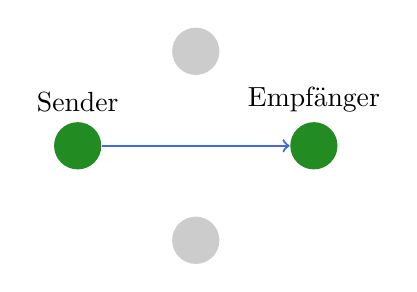
\begin{tikzpicture}
			% Nodes
			\node[fill=ForestGreen, circle, minimum size=6mm, label=above:{Sender}] (A) at (0,0) {};
			\node[fill=ForestGreen, circle, minimum size=6mm, label=above:{Empfänger}] (B) at (3,0) {};
			% Other nodes (not involved)
			\node[fill=Gray!40, circle, minimum size=6mm] (C) at (1.5,1.2) {};
			\node[fill=Gray!40, circle, minimum size=6mm] (D) at (1.5,-1.2) {};
			% Arrows
			\draw[->, thick, RoyalBlue] (A) -- (B);
		\end{tikzpicture}
		\caption{Unicast: 1:1}
	\end{subfigure}%
	% Multicast
	\begin{subfigure}[b]{0.3\textwidth}
		\centering
		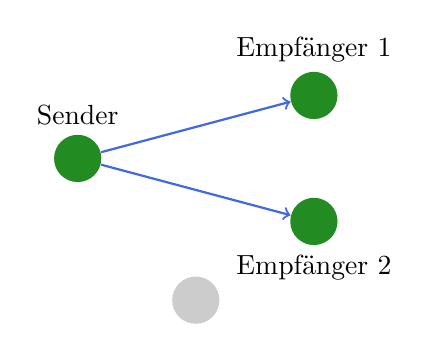
\begin{tikzpicture}
			% Nodes
			\node[fill=ForestGreen, circle, minimum size=6mm, label=above:{Sender}] (A) at (0,0) {};
			\node[fill=ForestGreen, circle, minimum size=6mm, label=above:{Empfänger 1}] (B) at (3,0.8) {};
			\node[fill=ForestGreen, circle, minimum size=6mm, label=below:{Empfänger 2}] (C) at (3,-0.8) {};
			% Other node (not involved)
			\node[fill=Gray!40, circle, minimum size=6mm] (D) at (1.5,-1.8) {};
			% Arrows
			\draw[->, thick, RoyalBlue] (A) -- (B);
			\draw[->, thick, RoyalBlue] (A) -- (C);
		\end{tikzpicture}
		\caption{Multicast: 1:n (Gruppe)}
	\end{subfigure}%
	% Broadcast
	\begin{subfigure}[b]{0.3\textwidth}
		\centering
		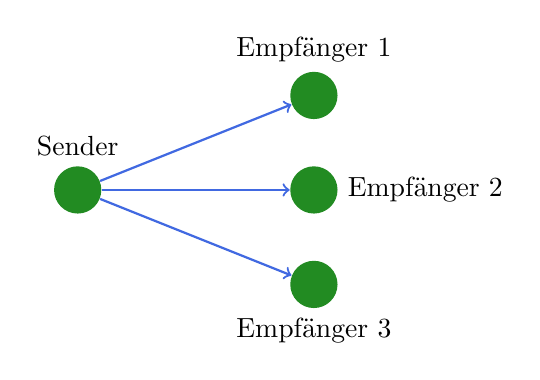
\begin{tikzpicture}
			% Nodes
			\node[fill=ForestGreen, circle, minimum size=6mm, label=above:{Sender}] (A) at (0,0) {};
			\node[fill=ForestGreen, circle, minimum size=6mm, label=above:{Empfänger 1}] (B) at (3,1.2) {};
			\node[fill=ForestGreen, circle, minimum size=6mm, label=right:{Empfänger 2}] (C) at (3,0) {};
			\node[fill=ForestGreen, circle, minimum size=6mm, label=below:{Empfänger 3}] (D) at (3,-1.2) {};
			% Arrows
			\draw[->, thick, RoyalBlue] (A) -- (B);
			\draw[->, thick, RoyalBlue] (A) -- (C);
			\draw[->, thick, RoyalBlue] (A) -- (D);
		\end{tikzpicture}
		\caption{Broadcast: 1:alle}
	\end{subfigure}
	\caption{Unicast, Multicast und Broadcast: Übertragungsarten im Netzwerk}
	\label{fig:unicast-multicast-broadcast}
\end{figure}

\begin{myexercise}[Alltagsbeispiele für Übertragungsarten im Netzwerk]
	Welche Art der Datenübertragung verwenden die folgenden Alltagssituationen?
	\begin{itemize}
		\item Whatsapp-Nachricht an eine befreundete Person
		\item Lautsprecherdurchsage im gesamten Flughafen
		\item Lautsprecherdurchsage auf dem Gleis bei der SBB
		\item Info-Box im Intranet
		\item Frage einer Person an eine Gruppe der Klasse
		\item Email der Schulleitung an alle Eltern
	\end{itemize}
	\begin{myanswer}
		\begin{itemize}
			\item Whatsapp-Nachricht an eine befreundete Person: \textbf{Unicast} (1:1)
			\item Lautsprecherdurchsage im gesamten Flughafen: \textbf{Broadcast} (an alle Anwesenden im Flughafen)
			\item Lautsprecherdurchsage auf dem Gleis bei der SBB: \textbf{Multicast} (an alle auf dem Gleis aber nicht an alle Anwesenden im Bahnhof)
			\item Info-Box im Intranet: \textbf{Broadcast} (an alle Nutzer des Intranets)
			\item Frage an eine Gruppe der Klasse: \textbf{Multicast} (an eine bestimmte Gruppe, z.B. die Teammitglieder eines Projekts)
			\item Email der Schulleitung an alle Eltern: \textbf{Multicast} (an eine definierte Empfängergruppe)
		\end{itemize}
	\end{myanswer}
\end{myexercise}


\section{\texorpdfstring{\textcolor{\networkLayerColor}{Vermittlungsschicht / Internetschicht}}{Vermittlungsschicht / Internetschicht}}
Die Übertragungssicherungsschicht befasst sich mit der stabilen Übertragung von Daten zwischen zwei Rechnern. Wofür sie jedoch nicht zuständig ist, ist die Adressierung und Identifizierung von Computern im Netzwerk. Diesem Aspekt ist die Internetschicht gewidmet.

\subsection{IP-Adressen}

Eine \acrfull{IP}-Adresse ist eine Netzwerk-Adresse eines Computers. Somit ist sie in gewisser Weise der Wohnadresse einer Person ähnlich. Häufig werden \gls{IP}-Adressen noch im \textbf{IPv4}-Format angegeben: Dieses besteht aus 4 bytes, also 4 Zahlen von 0 bis 255. Die \gls{IP}v4-Adresse wird meist dezimal angegeben (beispielsweise \texttt{192.168.0.1}).

Häufig wird zwischen der \textbf{lokalen} und der \textbf{globalen} \gls{IP}-Adresse unterschieden:
\begin{itemize}
	\item Die \textbf{lokale} \gls{IP}-Adresse (auch private \gls{IP}-Adresse genannt) ist die Adresse eines Computers innerhalb eines lokalen Netzwerks (z.B. im Heimnetzwerk oder Firmennetzwerk). Diese Adresse ist nur innerhalb dieses lokalen Netzwerks gültig und kann von anderen Computern im Internet nicht direkt erreicht werden.
	\item Die \textbf{globale} \gls{IP}-Adresse (auch öffentliche \gls{IP}-Adresse genannt) ist die Adresse eines Computers im gesamten Internet. Diese Adresse ist weltweit eindeutig und ermöglicht es Computern, miteinander über das Internet zu kommunizieren. Die globale \gls{IP}-Adresse wird in der Regel von einem Internetdienstanbieter (\gls{ISP}) zugewiesen.
\end{itemize}

Der Grund, warum es lokale und globale \gls{IP}-Adressen gibt, liegt darin, dass es nicht genügend globale \gls{IP}-Adressen für alle Geräte auf der Welt gibt. Durch die Verwendung von lokalen \gls{IP}-Adressen in privaten Netzwerken können viele Geräte dieselbe lokale Adresse verwenden, solange sie sich in unterschiedlichen Netzwerken befinden. Der Router in einem lokalen Netzwerk übernimmt dann die Aufgabe, die Kommunikation zwischen den lokalen Geräten und dem Internet zu koordinieren, indem er die lokalen Adressen in die globale Adresse übersetzt (dies wird als \gls{NAT} bezeichnet). Weitere Informationen zu \gls{NAT} sowie Port Forwarding finden Sie in \cref{app:nat_port_forwarding}. Ein Beispiel für die Umwandlung von lokalen in globale \gls{IP}-Adressen ist in \cref{fig:nat-example} dargestellt.

\begin{figure}[H]
	\centering
	\begin{subfigure}[b]{\textwidth}
		\centering
		\begin{tikzpicture}[
				base/.style={rectangle, draw, minimum width=2.5cm, minimum height=1cm, text=white, rounded corners, text width=2.5cm, align=center, inner sep=8pt},
				device/.style={base, fill=ForestGreen},
				router/.style={base, fill=\networkLayerColor},
				server/.style={base, fill=Crimson},
				arrow/.style={-Stealth, thick, text width=3cm, align=center}
			]

			% Nodes
			\node[device] (client) {Client\\\texttt{192.168.0.10}};
			\node[device, below=.2cm of client] (client2) {Client\\\texttt{192.168.0.11}};
			\node[device, below=.2cm of client2] (client3) {Client\\\texttt{192.168.0.12}};
			\node[router, right=3cm of client2] (nat) {Router\\\texttt{80.152.43.21}};
			\node[server, right=3cm of nat] (web) {Webserver\\\texttt{159.233.1.22}};

			\node[draw=Crimson!60, rounded corners, thick, dashed, inner sep=6pt, fit=(client)(client2)(client3)(nat)] (lan2area){};

			% Label boxes
			\node[red, align=left, font=\small, anchor=south west] at (lan2area.north west) {Lokales Netzwerk};
			\node[below=0.5cm of web, text width=2.5cm, align=center, font=\small] {Internet};

			% Arrows
			\draw[arrow] (client.east) -- (nat.west) node[midway, above, text=black] {Anfrage von\\\texttt{192.168.0.10}};
		\end{tikzpicture}
		\caption{Schritt 1: Client sendet Anfrage}
	\end{subfigure}

	\begin{subfigure}[b]{\textwidth}
		\centering
		\begin{tikzpicture}[
				base/.style={rectangle, draw, minimum width=2.5cm, minimum height=1cm, text=white, rounded corners, text width=2.5cm, align=center, inner sep=8pt},
				device/.style={base, fill=ForestGreen},
				router/.style={base, fill=\networkLayerColor},
				server/.style={base, fill=Crimson},
				arrow/.style={-Stealth, thick, text width=3cm, align=center}
			]

			% Nodes
			\node[device] (client) {Client\\\texttt{192.168.0.10}};
			\node[device, below=.2cm of client] (client2) {Client\\\texttt{192.168.0.11}};
			\node[device, below=.2cm of client2] (client3) {Client\\\texttt{192.168.0.12}};
			\node[router, right=3cm of client2] (nat) {Router\\\texttt{80.152.43.21}};
			\node[server, right=3cm of nat] (web) {Webserver\\\texttt{159.233.1.22}};

			\node[draw=Crimson!60, rounded corners, thick, dashed, inner sep=6pt, fit=(client)(client2)(client3)(nat)] (lan2area){};

			% Label boxes
			\node[red, align=left, font=\small, anchor=south west] at (lan2area.north west) {Lokales Netzwerk};
			\node[below=0.5cm of web, text width=2.5cm, align=center, font=\small] {Internet};

			% Arrows
			\draw[arrow] (nat.east) -- (web.west) node[midway, above, text=black] {Anfrage von\\\texttt{80.152.43.21} \faCheck};

			% NAT table
			\node[below=0.1cm of nat, text width=3.5cm, font=\tiny, inner sep=8pt, draw, rounded corners, fill=\networkLayerColor!10] (natTable) {
				\textbf{\acrshort{NAT}-Tabelle}
				\begin{tabular}{p{1.4cm}|p{1.4cm}}
					\textbf{Lokal} & \textbf{Global} \\
					\midrule\midrule
					192.168.0.10   & 80.152.43.21    \\
				\end{tabular}
			};
		\end{tikzpicture}
		\caption{Schritt 2: Router übersetzt lokale IP und sendet Anfrage}
	\end{subfigure}

	\begin{subfigure}[b]{\textwidth}
		\centering
		\begin{tikzpicture}[
				base/.style={rectangle, draw, minimum width=2.5cm, minimum height=1cm, text=white, rounded corners, text width=2.5cm, align=center, inner sep=8pt},
				device/.style={base, fill=ForestGreen},
				router/.style={base, fill=\networkLayerColor},
				server/.style={base, fill=Crimson},
				arrow/.style={-Stealth, thick, text width=3cm, align=center}
			]

			% Nodes
			\node[device] (client) {Client\\\texttt{192.168.0.10}};
			\node[device, below=.2cm of client] (client2) {Client\\\texttt{192.168.0.11}};
			\node[device, below=.2cm of client2] (client3) {Client\\\texttt{192.168.0.12}};
			\node[router, right=3cm of client2] (nat) {Router\\\texttt{80.152.43.21}};
			\node[server, right=3cm of nat] (web) {Webserver\\\texttt{159.233.1.22}};

			\node[draw=Crimson!60, rounded corners, thick, dashed, inner sep=6pt, fit=(client)(client2)(client3)(nat)] (lan2area){};

			% Label boxes
			\node[red, align=left, font=\small, anchor=south west] at (lan2area.north west) {Lokales Netzwerk};
			\node[below=0.5cm of web, text width=2.5cm, align=center, font=\small] {Internet};

			% Arrows
			\draw[arrow] (web.west) -- (nat.east) node[midway, below, text=black] {Antwort an\\\texttt{80.152.43.21}};

			% NAT table
			\node[below=0.1cm of nat, text width=3.5cm, font=\tiny, inner sep=8pt, draw, rounded corners, fill=\networkLayerColor!10] (natTable) {
				\textbf{\acrshort{NAT}-Tabelle}
				\begin{tabular}{p{1.4cm}|p{1.4cm}}
					\textbf{Lokal} & \textbf{Global} \\
					\midrule\midrule
					192.168.0.10   & 80.152.43.21    \\
				\end{tabular}
			};
		\end{tikzpicture}
		\caption{Schritt 3: Webserver sendet Antwort}
	\end{subfigure}

	\begin{subfigure}[b]{\textwidth}
		\centering
		\begin{tikzpicture}[
				base/.style={rectangle, draw, minimum width=2.5cm, minimum height=1cm, text=white, rounded corners, text width=2.5cm, align=center, inner sep=8pt},
				device/.style={base, fill=ForestGreen},
				router/.style={base, fill=\networkLayerColor},
				server/.style={base, fill=Crimson},
				arrow/.style={-Stealth, thick, text width=3cm, align=center}
			]

			% Nodes
			\node[device] (client) {Client\\\texttt{192.168.0.10}};
			\node[device, below=.2cm of client] (client2) {Client\\\texttt{192.168.0.11}};
			\node[device, below=.2cm of client2] (client3) {Client\\\texttt{192.168.0.12}};
			\node[router, right=3cm of client2] (nat) {Router\\\texttt{80.152.43.21}};
			\node[server, right=3cm of nat] (web) {Webserver\\\texttt{159.233.1.22}};

			\node[draw=Crimson!60, rounded corners, thick, dashed, inner sep=6pt, fit=(client)(client2)(client3)(nat)] (lan2area){};

			% Label boxes
			\node[red, align=left, font=\small, anchor=south west] at (lan2area.north west) {Lokales Netzwerk};
			\node[below=0.5cm of web, text width=2.5cm, align=center, font=\small] {Internet};

			% Arrows
			\draw[arrow] (nat.west) -- (client.east) node[midway, below, text=black] {Antwort an\\\texttt{192.168.0.10} \faCheck};

			% NAT table
			\node[below=0.1cm of nat, text width=3.5cm, font=\tiny, inner sep=8pt, draw, rounded corners, fill=\networkLayerColor!10] (natTable) {
				\textbf{\acrshort{NAT}-Tabelle}
				\begin{tabular}{p{1.4cm}|p{1.4cm}}
					\textbf{Lokal} & \textbf{Global} \\
					\midrule\midrule
					192.168.0.10   & 80.152.43.21    \\
				\end{tabular}
			};
		\end{tikzpicture}
		\caption{Schritt 4: Router übersetzt globale IP zurück und sendet Antwort}
	\end{subfigure}

	\caption{Beispiel für die Umwandlung von lokalen in globale \gls{IP}-Adressen mittels \gls{NAT}}
	\label{fig:nat-example}
\end{figure}

Die lokale Netzwerk-Adresse eines Computers wird häufig automatisch von einem \gls{DHCP}-Server zugewiesen, welcher in der Regel im Router integriert ist. Der \gls{DHCP}-Server verwaltet dabei einen Pool von verfügbaren \gls{IP}-Adressen und weist jedem Computer, der sich mit dem Netzwerk verbindet, eine freie Adresse aus diesem Pool zu. Dies geschieht automatisch und vereinfacht die Verwaltung von \gls{IP}-Adressen in einem Netzwerk erheblich.

\begin{myexercise}[Eigene lokale und globale \gls{IP} herausfinden]\label{ex:meine-ip}
	Finden Sie Ihre eigene lokale \gls{IP}v4-Adresse heraus.
	\begin{itemize}
		\item[\faApple] \textbf{MacOS}: Öffnen Sie das \textbf{Terminal} (dieses können Sie via Spotlight-Suche finden: \keys{\cmd + \SPACE}). Tippen Sie im Terminal: \commandbox*|ipconfig getifaddr en0|
		\item[\faWindows] \textbf{Windows}: Öffnen Sie die \textbf{Eingabeaufforderung} (diese können Sie finden durch Drücken der \keys{\faWindows}-Taste, danach Suche nach dem Programm \texttt{cmd} oder Eingabeaufforderung). Tippen Sie in der Eingabeaufforderung: \commandbox*|ipconfig|
	\end{itemize}
	Ihre eigene globale \gls{IP}v4-Adresse können Sie beispielsweise über die Webseite \url{https://www.whatismyip.com/} herausfinden.
\end{myexercise}

\begin{mychallenge}[\commandbox*|ping| im lokalen Netzwerk]
	In vielen Schul-\glspl{WLAN} ist das Anpingen von anderen Geräten aus Sicherheitsgründen deaktiviert. Wechseln Sie daher in ein anderes Netzwerk, z.B. den Hotspot Ihres Smartphones, um die Übung durchzuführen.

	Tauschen Sie zu zweit ihre lokale \gls{IP}v4-Adresse aus (siehe \cref{ex:meine-ip}) und überprüfen Sie, ob Sie sich gegenseitig im lokalen Netzwerk anpingen können. Verwenden Sie dazu den Befehl \commandbox*|ping [lokale IP-Adresse des anderen Teilnehmers]| im Terminal (MacOS) oder in der Eingabeaufforderung (Windows).
\end{mychallenge}



\begin{mychallenge}
	Führen Sie folgendes Skript in Python aus, um zu überprüfen, ob Sie dieselbe lokale und globale \gls{IP}-Adresse wie in \cref{ex:meine-ip} herausgefunden haben:
	\lstinputlisting{Grundlagen_Info/07_Netzwerke/Code/get_net_configs.py}
\end{mychallenge}

\begin{mychallenge}[ARP-Scan im lokalen Netzwerk]
	Falls Sie wissen wollen, welche anderen Geräte im lokalen Netzwerk existieren, können Sie ein \gls{ARP}-Scan mit dem Programm \texttt{arp-scan} durchführen. Am einfachsten kann das Programm \texttt{arp-scan} auf MacOS mit Homebrew installiert werden. Führen Sie dazu im Terminal folgenden Befehl aus:
	\commandbox*|brew install arp-scan|

	Führen Sie danach folgenden Befehl aus, um alle Geräte im lokalen Netzwerk zu scannen:
	\commandbox*|sudo arp-scan --localnet --interface=en0|

	Die Option \commandbox*|--localnet| sorgt dafür, dass nur das lokale Netzwerk gescannt wird. Die Option \commandbox*|--interface=en0| bedeutet, dass die Netzwerkschnittstelle \commandbox|en0| (normalerweise WLAN) verwendet wird.

	Ihre \gls{ARP}-Tabelle wird danach mit den gefundenen Geräten aktualisiert. Sie können die Tabelle mit dem Befehl \commandbox*|arp -a| (MacOS) bzw. \commandbox*|arp -a| (Windows) anzeigen.
\end{mychallenge}

\begin{myexercise}
	Bringen Sie folgende \gls{IP}v4-Adresse in die dezimale Schreibweise:

	\texttt{11000000.10101000.00000001.00000001}

	\begin{myanswer}
		\begin{itemize}
			\item $11000000_2 = 192_{10}$
			\item $10101000_2 = 168_{10}$
			\item $00000001_2 = 1_{10}$
			\item $00000001_2 = 1_{10}$
		\end{itemize}
		$\rightarrow \text{Dezimale Schreibweise: }\texttt{192.168.1.1}$
	\end{myanswer}
\end{myexercise}

\begin{myexercise}\label{ex:ipv4}
	Wie viele \gls{IP}v4-Adressen gibt es?
	\begin{myanswer}
		\begin{itemize}
			\item $4\cdot 1 \text{ byte} = 4\cdot 8 \text{ bits} = 32 \text{ bits}$
			\item $2^{32} \approx 4 \text{ Milliarden Adressen}$
			\item $\rightarrow$ zu wenig, da es heute deutlich mehr als 4 Milliarden Geräte gibt!
		\end{itemize}
	\end{myanswer}
\end{myexercise}
Wie wir in \cref{ex:ipv4} gesehen haben, gibt es zu wenige Adressen bei \gls{IP}v4. Daher wird \gls{IP}v4 graduell durch einen neuen Standard abgelöst, \textbf{\gls{IP}v6}, in welchem jede Adresse über 128 Bits verfügt, womit fast unendlich viele Geräte adressiert werden können.

\begin{mydefinition}[\gls{IP}v6-Adressen]
Eine \gls{IP}v6-Adresse besteht aus 128 Bits, wobei die 128 Bits in 8 Gruppen zu je 16 Bits aufgeteilt werden, welche durch Doppelpunkte getrennt sind. Zur einfacheren Lesbarkeit werden \gls{IP}v6-Adressen in hexadezimaler Schreibweise angegeben, also mit den Ziffern 0-9 und A-F. Eine typische \gls{IP}v6-Adresse sieht beispielsweise folgendermassen aus: \texttt{2001:0db8:85a3:0000:0000:8a2e:0370:7334}. Zur Vereinfachung können führende Nullen in einer Gruppe weggelassen werden, sowie aufeinanderfolgende Gruppen mit dem Wert 0 durch \enquote{::} ersetzt werden. Somit kann die obige Adresse auch als \texttt{2001:db8:85a3::8a2e:370:7334} geschrieben werden. Doppelte Doppelpunkt-Kürzungen sind jedoch nicht erlaubt (also z.B. \texttt{2001::85a3::8a2e:370:7334} ist ungültig).
\end{mydefinition}

\begin{myexercise}
	Wie viele Adressen gibt es bei IPv6?
	\begin{myanswer}
		\[2^{128} \approx 3.4\cdot 10^{38}\]
	\end{myanswer}
\end{myexercise}

\begin{myexercise}
	Entscheiden Sie für jede der folgenden Adressen, ob es sich um eine gültige \gls{IP}v4-Adresse, um eine gültige \gls{IP}v6-Adresse oder um keine gültige \gls{IP}-Adresse handelt:
	\begin{itemize}
		\item \texttt{256.100.50.25}
		\item \texttt{192.168.1.1}
		\item \texttt{10.0.0}
		\item \texttt{2001:0db8:85a3:0000:0000:8a2e:0370:7334}
		\item \texttt{2001:db8::1}
		\item \texttt{1234:5678:9abc:def0:1234:5678:9abc:def0}
		\item \texttt{2001:db8:::1}
		\item \texttt{192.168.1.1.1}
	\end{itemize}
	\begin{myanswer}
		\begin{itemize}
			\item Keine gültige \gls{IP}-Adresse (erstes Byte > 255)
			\item Gültige \gls{IP}v4-Adresse
			\item Keine gültige \gls{IP}-Adresse (falsches IPv4-Format)
			\item Gültige \gls{IP}v6-Adresse
			\item Gültige \gls{IP}v6-Adresse
			\item Gültige \gls{IP}v6-Adresse
			\item Keine gültige \gls{IP}-Adresse (mehrfache Verwendung von \enquote{::})
			\item Keine gültige \gls{IP}-Adresse (zu viele Oktette)
		\end{itemize}
	\end{myanswer}
\end{myexercise}

\begin{myexercise}
	Was ist die grösste mögliche \gls{IP}v4-Adresse in dezimaler Schreibweise? Was ist die grösste mögliche \gls{IP}v6-Adresse in hexadezimaler Schreibweise?
	\begin{myanswer}
		\begin{itemize}
			\item Grösste mögliche \gls{IP}v4-Adresse: \texttt{255.255.255.255}
			\item Grösste mögliche \gls{IP}v6-Adresse: \texttt{ffff:ffff:ffff:ffff:ffff:ffff:ffff:ffff}
		\end{itemize}
	\end{myanswer}
\end{myexercise}

\begin{myremark}[IPv4 vs. IPv6]
	In der Praxis werden \gls{IP}v4-Adressen immer noch am häufigsten verwendet, da viele ältere Geräte und Netzwerke nur \gls{IP}v4 unterstützen. Allerdings wird \gls{IP}v6 zunehmend wichtiger, da die Anzahl der Geräte im Internet stetig zunimmt und der Adressraum von \gls{IP}v4 nicht mehr ausreicht. Viele moderne Betriebssysteme und Netzwerke unterstützen bereits \gls{IP}v6, und es wird erwartet, dass in Zukunft immer mehr Geräte auf \gls{IP}v6 umsteigen werden. Um den Mangel an \gls{IP}v4-Adressen zu beheben, werden auch Techniken wie \acrfull{NAT}, \acrfull{PAT} und Port Forwarding eingesetzt, die es ermöglichen, mehrere Geräte hinter einer einzigen öffentlichen \gls{IP}-Adresse zu betreiben (s. \cref{app:nat_port_forwarding} für weitere Informationen zu \acrshort{NAT}, \acrshort{PAT} und Port Forwarding).
\end{myremark}

\subsection{Netzmasken \& Subnetze}
\textbf{Subnetzwerke} verbinden --- wie es der Name sagt --- mehrere Hosts zu einem (Sub-)Netzwerk. Dabei gehören mehrere Geräte zum gleichen Subnetz, falls sie:
\begin{itemize}
	\item Physisch miteinander verbunden sind (via Kabel, \gls{WLAN}, etc.)
	\item Die gleiche Subnetzmaske teilen (später mehr dazu)
\end{itemize}

Eine (Sub-)Netzmaske hat fast dasselbe Format wie eine \gls{IP}-Adresse und fasst mehrere \glspl{IP} zu einer Gruppe, d.h. einem Subnetz zusammen. Die Subnetzmaske gibt an, wie viele Stellen einer \gls{IP}-Adresse innerhalb eines Subnetzes gleich sein müssen. Sie besteht immer aus zwei \glspl{IP}-Adressen, wobei die erste \gls{IP}-Adresse einer gültigen Adresse innerhalb des Subnetzes entspricht, und die zweite \gls{IP}-Adresse vorgibt, wie stark eine weitere \gls{IP}-Adresse von der ersten \gls{IP}-Adresse abweichen dürfte, damit sie immer noch zum selben Netz gehört.

\begin{myexample}[Subnetzmasken]\label{example:subnet}
Gegeben sei folgende Subnetzmaske:
\begin{table}[H]
	\centering
	\begin{tabular}{r|l|l}
		                                     & Dezimal                & Binär                                                                 \\\midrule\midrule
		\acrshort{IP}-Adresse von Computer 1 & \texttt{159.233.1.22}  & \texttt{\textcolor{ForestGreen}{10011111.11101001.00000001}.00010110} \\\midrule
		\acrshort{IP}-Adresse von Computer 2 & \texttt{159.233.1.1}   & \texttt{\textcolor{ForestGreen}{10011111.11101001.00000001}.00000001} \\\midrule
		Subnetzmaske                         & \texttt{255.255.255.0} & \texttt{\textcolor{ForestGreen}{11111111.11111111.11111111}.00000000}
	\end{tabular}
	\caption{Beispiel einer Subnetzmaske mit zwei IP-Adressen}
	\label{table:ex-subnet}
\end{table}
Um herauszufinden, ob die IP-Adressen von Computer 1 und Computer 2 zum selben Netzwerk gehören, muss überprüft werden, ob die binäre IP-Adresse an all denjenigen Stellen gleich ist, wo die Subnetzmaske = \enquote{1} ist (also an allen grün markierten Stellen in \cref{table:ex-subnet}). In diesem Beispiel bedeutet dies, dass alle \gls{IP}-Adressen, welche mit \texttt{159.233.1.[...]} beginnen zum selben Netzwerk gehören.
\end{myexample}


\begin{myexercise}[Geräte zu Subnetzen zuordnen]
	\begin{table}[H]
		\centering
		\begin{tabular}{l|l|l|m{2cm}}

			\textbf{Eigene \gls{IP}} & \textbf{Netzmaske} & \textbf{Ziel-\gls{IP}} & \textbf{Gleiches \newline Subnetz?} \\\midrule\midrule

			213.45.19.89             & 255.255.255.0      & 213.45.17.89           & \fldT                               \\\midrule

			213.45.19.89             & 255.255.0.0        & 213.45.17.89           & \fldT                               \\\midrule

			88.100.11.17             & 255.255.255.0      & 88.100.11.254          & \fldT                               \\\midrule

			88.100.11.17             & 0.0.0.0            & 213.45.19.89           & \fldT                               \\\midrule

			10.0.0.0                 & 255.255.255.252    & 10.0.0.1               & \fldT                               \\\midrule
			1.2.3.0                  & 255.255.255.252    & 1.2.3.5                & \fldT
		\end{tabular}
	\end{table}
	\begin{itemize}
		\item $\rightarrow$ \gls{IP}s dürfen sich nur an denjenigen Stellen unterscheiden, wo in der Maske (binär!) Nullen stehen.
		\item Umrechner dezimal $\rightarrow$ binär: \url{https://oinf.ch/interactive/ips-und-netzmaske/}
	\end{itemize}
	\begin{myanswer}

		\begin{table}[H]
			\centering
			\begin{tabular}{l|l|l|l}

				\textbf{Eigene IP} & \textbf{Netzmaske} & \textbf{Ziel-IP}                       & \textbf{Gleiches Subnetz?}     \\\midrule\midrule

				213.45.19.89       & 255.255.255.0      & 213.45.\textcolor{red}{17}.89          & Nein                           \\\midrule

				213.45.19.89       & 255.255.0.0        & \textcolor{ForestGreen}{213.45}.17.89  & Ja                             \\\midrule

				88.100.11.17       & 255.255.255.0      & \textcolor{ForestGreen}{88.100}.11.254 & Ja                             \\\midrule

				88.100.11.17       & 0.0.0.0            & 213.45.19.89                           & Ja (alles \faCheck)            \\\midrule

				10.0.0.0           & 255.255.255.252    & 10.0.0.1                               & Ja ($252_{10}=11111100_{2}$)   \\\midrule
				1.2.3.0            & 255.255.255.252    & 1.2.3.5                                & Nein ($252_{10}=11111100_{2}$)
			\end{tabular}
		\end{table}
	\end{myanswer}
\end{myexercise}

\begin{myexercise}[Subnetzgrösse berechnen]
	Typischerweise beginnen alle \gls{IP}-Adressen, die auf das lokale Netzwerk (=das Netzwerk, in dem sich der eigene Computer befindet) mit \texttt{192.168.xxx.xxx}. Die Subnetzmaske lautet also \texttt{255.255.0.0}. Wie viele Hosts haben in so einem Netzwerk Platz? Schreiben Sie die Subnetzmaske binär auf und rechnen Sie aus, wie viele unterschiedliche Geräte sich in diesem lokalen Netzwerk befinden können.
	\begin{myanswer}
		Zwei Bytes (die zwei letzten Byte-Gruppen) der Subnetzmaske sind reserviert für unterschiedliche Kombinationen von \gls{IP}-Adressen. Es können sich daher bis zu $2^{16}$ = 65'536 Hosts in einem solchen lokalen Netzwerk befinden.
	\end{myanswer}
\end{myexercise}

\begin{myexercise}[Subnetzmasken zuordnen]
	Sechs Subnetze sind gegeben durch je eine Netzmaske und eine IP eines sich darin befindenden Rechners. Entscheiden Sie für jede links aufgeführte IP, zu welchen Subnetzen der entsprechende Rechner gehört.\vspace{-.2cm}

	\begin{table}[H]
		\centering
		\small
		\begin{tabular}{m{2cm}||m{1.5cm}|m{1.5cm}|m{1.5cm}|m{1.5cm}|m{1.5cm}|m{1.5cm}}
			\textbf{Netzmaske Subnetz} & \multicolumn{2}{c|}{255.255.255.0} & \multicolumn{2}{c|}{255.255.0.0} & \multicolumn{2}{c}{255.255.255.240}                               \\
			\midrule
			IP                         & 3.4.5.6                            & 3.3.3.3                          & 3.4.5.6                             & 3.3.3.3 & 3.4.5.6 & 3.3.3.3 \\
			\midrule\midrule
			3.3.3.4                    & \fldT                              & \fldT                            & \fldT                               & \fldT   & \fldT   & \fldT   \\\midrule
			4.4.4.3                    & \fldT                              & \fldT                            & \fldT                               & \fldT   & \fldT   & \fldT   \\\midrule
			3.4.5.99                   & \fldT                              & \fldT                            & \fldT                               & \fldT   & \fldT   & \fldT   \\\midrule
			3.3.4.4                    & \fldT                              & \fldT                            & \fldT                               & \fldT   & \fldT   & \fldT   \\\midrule
			3.4.7.7                    & \fldT                              & \fldT                            & \fldT                               & \fldT   & \fldT   & \fldT   \\\midrule
			3.3.3.17                   & \fldT                              & \fldT                            & \fldT                               & \fldT   & \fldT   & \fldT   \\
		\end{tabular}
	\end{table}
	\begin{center}
		\vspace{-.5cm}Überprüfen: \url{https://oinf.ch/interactive/ips-und-netzmaske/}\vspace{-.2cm}
	\end{center}
	\begin{myanswer}
		\begin{table}[H]
			\centering
			\small
			\begin{tabular}{m{2cm}||m{1.5cm}|m{1.5cm}|m{1.5cm}|m{1.5cm}|m{1.5cm}|m{1.7cm}}
				\textbf{Netzmaske Subnetz} & \multicolumn{2}{c|}{255.255.255.0} & \multicolumn{2}{c|}{255.255.0.0} & \multicolumn{2}{c}{255.255.255.240}                               \\
				\midrule
				IP                         & 3.4.5.6                            & 3.3.3.3                          & 3.4.5.6                             & 3.3.3.3 & 3.4.5.6 & 3.3.3.3 \\
				\midrule\midrule
				3.3.3.4                    & Nein                               & Ja                               & Nein                                & Ja      & Nein    & Ja      \\\midrule
				4.4.4.3                    & Nein                               & Nein                             & Nein                                & Nein    & Nein    & Nein    \\\midrule
				3.4.5.99                   & Ja                                 & Nein                             & Ja                                  & Nein    & Nein    & Nein    \\\midrule
				3.3.4.4                    & Nein                               & Nein                             & Nein                                & Ja      & Nein    & Nein    \\\midrule
				3.4.7.7                    & Nein                               & Nein                             & Ja                                  & Nein    & Nein    & Nein    \\\midrule
				3.3.3.17                   & Nein                               & Ja                               & Nein                                & Ja      & Nein    & Nein    \\
			\end{tabular}
		\end{table}
	\end{myanswer}
\end{myexercise}


\begin{mydefinition}[\acrshort{CIDR}-Notation]
Das Netzwerk aus \cref{example:subnet} könnte dezimal angegeben werden wie folgt: 

\texttt{159.233.1.0/255.255.255.0}

Dabei bezeichnet der erste Teil die \gls{IP}-Adresse eines (gültigen) Hosts im Subnetz, und der zweite Teil bezeichnet die Subnetzmaske. 

Die Subnetzmaske wird häufig verkürzt in der sogenannten \gls{CIDR}-Schreibweise angegeben. Dabei wird die Subnetzmaske als \gls{IP}-Adresse gefolgt von einem Schrägstrich und der Anzahl der Einsen in der Subnetzmaske geschrieben. Die Subnetzmaske aus \cref{example:subnet} könnte somit auch als \texttt{159.233.1.0/24} geschrieben werden, da die Subnetzmaske 24 Einsen hat. 

Durch diese Schreibweise wird zudem schnell ersichtlich, wie gross das Netzwerk maximal sein darf. Die ersten 24 Bits der \gls{IP}-Adresse müssen immer gleich sein, daher bietet dieses Netzwerk Platz für maximal $2^{32-24} = 256$ unterschiedliche Hosts.
\end{mydefinition}


\begin{myexercise}[\acrshort{CIDR}-Notation]
	Geben Sie die folgenden Subnetzmasken in \gls{CIDR}-Notation an und notieren Sie die möglichen Adressebereiche für beide Netze 2 und 3, also die kleinste und grösste mögliche \gls{IP}-Adresse im jeweiligen Subnetz. Notieren Sie zudem, wie viele Hosts in jedem Subnetz Platz haben.
	\begin{itemize}
		\item \textbf{Netz 1} (Beispiel): \texttt{24.10.10.0} mit Netzmaske \texttt{255.255.255.240}
		\item \textbf{Netz 2}: \texttt{192.168.1.0} mit Netzmaske \texttt{255.255.255.192}
		\item \textbf{Netz 3}: \texttt{10.0.0.0} mit Netzmaske \texttt{255.128.0.0}
	\end{itemize}
	Um die Adressbereiche zu berechnen, können Sie den Online-Rechner unter \url{https://oinf.ch/interactive/ips-und-netzmaske/} verwenden.

	\begin{table}[H]
			\centering
			\begin{tabular}{l||m{2.5cm}|m{2.25cm}|m{2.5cm}|m{2.5cm}}
								&  \multirow{2}{2cm}{\textbf{\gls{CIDR}-\newline Schreibweise}}&\multirow{2}{2.25cm}{\textbf{Anzahl Hosts}} & \multicolumn{2}{l}{\textbf{Adressbereich}} \\\cmidrule{4-5}
								& & & \textbf{Start} & \textbf{Ende} \\
				\midrule\midrule
				Netz 1 & \texttt{24.10.10.0/28} & $2^{32-28} = 2^{4} = 16$ & \texttt{24.10.10.0} & \texttt{24.10.10.15} \\\midrule
				Netz 2  & \fldT & \fldT& \fldT           & \fldT         \\
				\midrule
				Netz 3 & \fldT & \fldT     & \fldT&\fldT       \\
				
			\end{tabular}
			\caption{Subnetzmasken in CIDR-Notation mit Anzahl Hosts und Adressbereichen}
		\end{table}
	\begin{myanswer}
		\begin{table}[H]
			\centering
			\begin{tabular}{l||l|m{2.5cm}|l|l}
								&  \multirow{2}{2cm}{\textbf{\gls{CIDR}-\newline Schreibweise}}&\multirow{2}{2.25cm}{\textbf{Anzahl Hosts}} & \multicolumn{2}{l}{\textbf{Adressbereich}} \\\cmidrule{4-5}
																& & & \textbf{Start} & \textbf{Ende} \\
												\midrule\midrule
												Netz 1 & \texttt{24.10.10.0/28} & $2^{32-28} = 2^{4} = 16$ & \texttt{24.10.10.0} & \texttt{24.10.10.15} \\\midrule
												Netz 2  & \texttt{192.168.1.0/26} & $2^{32-26} = 2^{6} = 64$& \texttt{192.168.1.0}           & \texttt{192.168.1.63}         \\
												\midrule
												Netz 3 & \texttt{10.0.0.0/9} & $2^{32-9} = 2^{23} = 8\,388\,608$     & \texttt{10.0.0.0}              & \texttt{10.127.255.255}       \\
												
			\end{tabular}
			\caption{Subnetzmasken in CIDR-Notation mit Anzahl Hosts und Adressbereichen}
		\end{table}
	\end{myanswer}
\end{myexercise}

\subsection{Router \& Gateways}
\begin{figure}[H]
	\centering
	\input{Grundlagen_Info/07_Netzwerke/Skript/Includes/chapter01_fig_subnets.tex}
	\caption{Zwei Subnetze (\gls{LAN} A und \gls{LAN} B) verbunden via Router}
	\label{fig:router-subnetze}
\end{figure}
Bis anhin haben wir gesehen, wie wir einzelne Rechner mittels einer IP adressieren und wie wir diese mittels Subnetzen oder Switches zu einem lokalen Netzwerk oder \gls{LAN} verbinden. Was, wenn wir jedoch zwei Subnetze zu einem grossen Netzwerk oder \gls{WAN} verbinden wollen? Genau dies geschieht im Internet, welches im Wesentlichen aus einem Netzwerk von Netzwerken besteht. Um mehrere Netzwerke miteinander zu verbinden, verwenden wir einen \textbf{Router}. Diesen schauen wir uns in diesem Abschnitt genauer an.

Ähnlich einer Haustür verbindet ein Router ein Subnetz (=Haus) mit der Aussenwelt, er befindet sich also an der Grenze zwischen zwei oder mehreren Subnetzen. Über die Routing-Tabelle kann ein Router entscheiden, auf welchen Weg ein Datenpaket an die Aussenwelt verschickt werden kann. Eine typische Routing-Tabelle enthält folgende Informationen:

\begin{itemize}
	\item \textbf{Ziel-\gls{IP} und Netzmaske}: Diese beiden Spalten definieren, welche Subnetze dem Router bekannt sind (sowohl eigenes Subnetz wie andere Subnetze).
	\item \textbf{Gateway} = Tor, Ein-/Ausfahrt: Der nächstgelegene Zielort, an den ein Paket geschickt werden muss, um eine gewisse Ziel-\gls{IP} zu erreichen. Das Gateway kann als eine Art \enquote{Tor zur Aussenwelt} angeschaut werden und ist häufig die \gls{IP}-Adresse des Routers der Ziel-\gls{IP}. Im Beispiel aus \cref{fig:router-subnetze} ist das Gateway für Pakete, die von \gls{LAN} A zu \gls{LAN} B geschickt werden sollen, die \gls{IP}-Adresse des Routers im \gls{LAN} A, also \texttt{192.168.1.1}.
	\item \textbf{Interface} = Schnittstelle: Die physikalische Schnittstelle am Router (z.B. Ethernet-Stecker, daher häufig abgekürzt, beispielsweise, \texttt{eth0} für das erste Ethernet-Interface oder \texttt{wlan0} für das erste \gls{WLAN}-Interface), über die eine Ziel-Adresse (Gateway) erreichbar ist. Im Beispiel aus \cref{fig:router-subnetze} ist das Interface für Pakete, die von \gls{LAN} A zu \gls{LAN} B geschickt werden sollen, das Ethernet-Kabel, das den Router mit dem \gls{LAN} A verbindet, also \texttt{eth0}.
\end{itemize}

Ein Beispiel einer minimalen Routing-Tabelle ist in \cref{table:routing} abgebildet.

\newcolumntype{S}{>{\small}p{5cm}<{\small}}   % small font, centered
\newcolumntype{T}{>{\ttfamily}l<{\ttfamily}}   % small font, monospace

\begin{table}[H]
	\centering
	\begin{tabular}{ T | T | T | T | S }
		\normalfont\textbf{Ziel-\gls{IP}} & \normalfont\textbf{Netzmaske} & \normalfont\textbf{Gateway} & \normalfont\textbf{Interface} & \normalsize\textbf{Kommentar}                                                                \\
		\midrule\midrule
		192.168.1.0                       & 255.255.255.0                 & 0.0.0.0                     & eth0                          & Direkt verbundenes \gls{LAN} \texttt{192.168.1.0/24} wird über Kabel \texttt{eth0} erreicht. \\\midrule
		192.168.2.0                       & 255.255.255.0                 & 0.0.0.0                     & eth1                          & Direkt verbundenes \gls{LAN} \texttt{192.168.2.0/24} wird über Kabel \texttt{eth1} erreicht. \\\midrule
		0.0.0.0                           & 0.0.0.0                       & 192.168.1.1                 & eth0                          & Standardroute ins Internet (\textit{default gateway})                                        \\
	\end{tabular}
	\caption{Beispiel einer Routing-Tabelle eines Routers, welcher sich in zwei \glspl{LAN} \texttt{192.168.1.0/24} und \texttt{192.168.2.0/24} befindet.}
	\label{table:routing}
\end{table}

Beim sogenannten \textit{default gateway} handelt es sich um die Standardroute, die verwendet wird, wenn keine spezifischere Route für eine Ziel-\gls{IP} in der Routing-Tabelle gefunden werden kann. In der Regel ist das Default Gateway die \gls{IP}-Adresse des Routers, der das Subnetz mit dem Internet verbindet.


\begin{myexercise}[Filius-Anwendung: Router \& Gateway]
	Schauen Sie sich das \href{https://www.youtube.com/watch?v=Kn8v_HrckUM&list=PLUfZiVdJui-57k0VcRecHX0JTEhOMgiKP}{Filius-Video Nummer 3} an. Laden Sie danach die Datei \enquote{\texttt{Filius-3.fls}} von Moodle herunter und bearbeiten Sie die darin enthaltene Netzwerkkonfiguration:
	\begin{itemize}
		\item Notieren Sie zuerst die beiden Netzwerke in \gls{CIDR}-Notation als Text.
		\item Konfigurieren Sie danach den Router korrekt, indem Sie die passenden \glspl{IP} für die beiden Interfaces des Routers vergeben.
		\item Stellen Sie die Switches als Wolke dar und entfernen Sie die Titel.
		\item Passen Sie die Gateways aller Clients an.
		\item Testen Sie die Konfiguration indem Sie einen \texttt{ping}-Befehl zwischen zwei Clients ausführen, die sich in unterschiedlichen Netzwerken befinden.
	\end{itemize}
\end{myexercise}

\begin{mychallenge}[Router \& Gateway verstehen]
	Lesen Sie mehr über die Aufgaben und Funktionsweise von Routern und Gateways, indem Sie \href{https://inf-schule.de/rechnernetze/filius/vernetzungrechnernetze/konzept_router}{diese Webseite} genau durchlesen.
\end{mychallenge}


\begin{myremark}[Automatische Zuweisung von \acrshort{IP}-Adressen via \acrshort{DHCP}]
	In der Praxis ist es unpraktisch, wenn jeder Computer in einem Netzwerk manuell mit einer \gls{IP}-Adresse konfiguriert werden muss. Daher wird häufig das \acrfull{DHCP} verwendet, um Computern automatisch eine \gls{IP}-Adresse zuzuweisen, wenn sie sich mit dem Netzwerk verbinden. 
	
	Ein \gls{DHCP}-Server verwaltet einen Pool von verfügbaren \gls{IP}-Adressen und weist diese dynamisch an Computer zu, die eine Verbindung zum Netzwerk herstellen. Dies erleichtert die Verwaltung von Netzwerken erheblich, insbesondere in Umgebungen mit vielen Geräten, wie z.B. in Unternehmen oder öffentlichen Netzwerken. 
\end{myremark}

\begin{myremark}[\gls{IP}-Reservierung]\label{remark:ip-reservation}
	Falls ein gewisses Gerät immer dieselbe lokale \gls{IP}-Adresse benötigt (z.B. ein Drucker oder ein Server), kann bei vielen Routern eine so genannte \textbf{\gls{IP}-Reservierung} eingerichtet werden, die sicherstellt, dass dieses Gerät immer dieselbe \gls{IP}-Adresse erhält, selbst wenn es sich erneut mit dem Netzwerk verbindet. Dies wird typischerweise durch die Zuordnung der \gls{MAC}-Adresse des Geräts zu einer bestimmten \gls{IP}-Adresse im \gls{DHCP}-Server des Routers erreicht. Eine \gls{IP}-Reservationstabelle könnte beispielsweise wie folgt aussehen:
	\begin{table}[H]
		\centering
		\begin{tabular}{l|l}
			\textbf{\gls{MAC}-Adresse}        & \textbf{Reservierte \gls{IP}-Adresse} \\\midrule\midrule
			\texttt{00:1A:2B:3C:4D:5E}           & \texttt{192.168.1.20} \\\midrule
			\texttt{11:22:33:44:55:66}           & \texttt{192.168.1.21} \\\midrule
			$\cdots$					 & $\dots$       \\
		\end{tabular}
		\caption{Beispiel einer \gls{IP}-Reservationstabelle}
	\end{table}
\end{myremark}

\subsection{\texorpdfstring{Zusammenfügen mehrerer \glspl{LAN} zum \gls{WAN} (Internet)}{Zusammenfügen mehrerer LANs zum WAN (Internet)}}
Stellen Sie sich vor, Sie möchten mehrere lokale Netzwerke (\glspl{LAN}) zu einem grossen Netzwerk (\gls{WAN}) verbinden, ähnlich wie es im Internet der Fall ist. Jedes \gls{LAN} soll dabei über einen Router mit dem \gls{WAN} verbunden werden. Eine kohärente Auswahl von IP-Adressen für jedes Netzwerk und die Router ist dabei entscheidend, um eine übersichtliche und funktionierende Netzwerkinfrastruktur zu gewährleisten.


\begin{myexercise}[Filius-Anwendung: Router \& Gateway]
	Schauen Sie sich (bei Bedarf) das \href{https://www.youtube.com/watch?v=Kn8v_HrckUM&list=PLUfZiVdJui-57k0VcRecHX0JTEhOMgiKP}{Filius-Video Nummer 4} an. Schauen Sie sich nach dem Video das etwas komplexere Netzwerk \enquote{\texttt{Filius 4 Routing Bugs.fls}} an, welches Sie von Moodle herunterladen können. Leider ist in diesem Netzwerk einiges kaputtgegangen und der Rechner \texttt{192.168.0.12} kann den Rechner \texttt{68.33.1.11} nicht mehr anpingen. Beheben Sie die Netzwerkkonfiguration, so dass die beiden Rechner sich wieder erreichen können. 
	\begin{itemize}
		\item Führen Sie zuerst einen \commandbox*|ping|-Befehl vom Rechner \texttt{192.168.0.12} zum Rechner \texttt{68.33.1.11} aus und beobachten Sie anhand der grün aufleuchtenden Striche, bis zu welchem Punkt die Pakete gesendet werden können.
		\item Setzen Sie bei den Routern korrekte Weiterleitungstabellen ein.
		\item Setzen Sie bei den Clients korrekte Gateways ein.
	\end{itemize}
\end{myexercise}

\section{\texorpdfstring{\textcolor{\transportLayerColor}{Transportschicht}}{Transportschicht}}
In der Transportschicht geht es, wie es der Name bereits sagt, darum, wie Daten von einem Host zum nächsten transportiert werden.

Die Daten, die zwischen zwei Computern übertragen werden, werden häufig auch als \textbf{Nutzdaten} oder \textit{payload} bezeichnet. Zu diesen Nutzdaten, die zwischen zwei Computern hin- und hergesandt werden sollen, kommen nun noch verschiedene weitere Daten dazu, so genannte \textbf{Metadaten}. Metadaten sind dazu zuständig, wichtige Informationen zu den Ursprungsdaten hinzuzufügen, in diesem Falle Daten, um den Transport der Daten zu ermöglichen. Diese Metadaten werden vom Übertragungs-Steuerungs-Protokoll (\gls{TCP}) zur Verfügung gestellt und genutzt, in einem so genannten \textit{Header} (siehe \cref{fig:tcp-header}).

\begin{figure}[H]
	\centering
	\input{Grundlagen_Info/07_Netzwerke/Skript/Includes/chapter01_table_tcpheader.tex}
	\caption{\gls{TCP}-Header (vereinfachte Darstellung)}
	\label{fig:tcp-header}
\end{figure}


Einige der wichtigsten Metadaten sind:

\begin{itemize}
	\item \textbf{Der Port} (von engl. \textit{port} = Hafen): Dies ist eine Zahl, mit der der Computer weiss, welche Anwendung (z.B. Mail, Browser, Gaming-Programm etc.) Daten verschickt. Ein Computer kann, wie Sie vermutlich wissen, gleichzeitig über mehrere Programme Daten von anderen Computern empfangen und an sie schicken: sie können beispielsweise gleichzeitig eine Nachricht über WhatsApp schicken und ein Video schauen. Damit der Computer weiss, welche Anwendung die Daten verschickt, versieht er die Daten typischerweise mit einem Port. Obschon Ports für jedes Programm frei gewählt werden können, werden für bekannte Protokolle typischerweise Standard-Portnummern verwendet (siehe \cref{tab:tcpPorts}).
	      \begin{table}[H]
		      \centering
		      \begin{tabular}{c||c|c}
			      \toprule
			      \textbf{Port} & \textbf{Anwendung} & \textbf{Verwendung}                   \\
			      \midrule
			      20            & \acrfull{FTP}      & Dateitransfer                         \\
			      21            & \acrfull{FTP}      & Befehlssteuerung                      \\
			      22            & \acrfull{SSH}      & Sichere Shell-Zugriffe                \\
			      25            & \acrfull{SMTP}     & E-Mail-Versand                        \\
			      53            & \acrfull{DNS}      & Namensauflösung                       \\
			      80            & \acrfull{HTTP}     & Webseiten-Abruf                       \\
			      110           & \acrfull{POP3}     & E-Mail-Abholung                       \\
			      143           & \acrfull{IMAP}     & E-Mail-Management                     \\
			      443           & \acrfull{HTTPS}    & Verschlüsselter Webseiten-Abruf       \\
			      993           & \acrfull{IMAP}     & E-Mail-Management über \acrshort{SSL} \\
			      995           & \acrfull{POP3}     & E-Mail-Abholung über \acrshort{SSL}   \\
			      \bottomrule
		      \end{tabular}
		      \caption{Gängige \gls{TCP}-Ports, Anwendungen und deren Verwendung}
		      \label{tab:tcpPorts}
	      \end{table}
	      Sowohl der \textit{Client} wie auch der \textit{Server} versehen die Daten mit jeweils einer Zahl, die für den Ursprungs-Port (\textit{Source Port}), respektive den Ziel-Port (\textit{Destination Port}) stehen.
	\item \textbf{Ziffern} für die \textit{Sequence} (Sequenz) und \textit{Acknowledgement} (Anerkennung) von Paketen, die die richtige Reihenfolge der gesendeten und erhaltenen Daten garantieren.
	\item Weitere Daten, die für den Transport notwendig sind.
\end{itemize}

\begin{myexercise}[Ports für \gls{HTTP}-Verbindungen]
	Testen Sie, was beim Aufrufen von \url{http://www.sbb.ch:80} und \url{http://www.sbb.ch:81} passiert. Erklären Sie den Unterschied.
	\begin{myanswer}
		\begin{itemize}
			\item \url{http://www.sbb.ch:80} funktioniert, da Port 80 der Standard-Port für HTTP-Verbindungen ist. Der Webserver der SBB hört auf diesem Port und kann daher die Anfrage verarbeiten und die Webseite ausliefern.
			\item \url{http://www.sbb.ch:81} funktioniert nicht, da Port 81 kein Standard-Port für HTTP-Verbindungen ist und der Webserver der SBB wahrscheinlich nicht auf diesem Port hört. Daher kann die Anfrage nicht verarbeitet werden und es wird keine Webseite ausgeliefert.
		\end{itemize}
	\end{myanswer}
\end{myexercise}

Nebst \gls{TCP} gibt es noch ein weiteres Protokoll in der Transportschicht, das \gls{UDP}. Im Gegensatz zu \gls{TCP} stellt \gls{UDP} keine zuverlässige Datenübertragung sicher, sondern sendet die Daten einfach los, ohne zu überprüfen, ob sie auch angekommen sind. Dies ist nützlich für Anwendungen, bei denen Geschwindigkeit wichtiger ist als Zuverlässigkeit, wie z.B. bei Online-Gaming oder Video-Streaming, oder auch für \gls{VPN}-Verbindungen.

\begin{mychallenge}[Weitere Port-Aufgaben]
	Lösen Sie die Socket- und Port-Aufgaben auf folgendem Link: \url{https://www.inf-schule.de/rechnernetze/anwendung/socketprogrammierung/Anfragen_an_einen_Server_Stellen}.
\end{mychallenge}

Zusätzlich zur Steuerung der Datenübertragung können \gls{TCP}-Metadaten genutzt werden, um die erste Verbindung zwischen zwei Computern herzustellen. Dies erfolgt typischerweise über das 3-Wege-Handschlag-Protokoll (siehe \cref{fig:threewayHandshake}).

\begin{figure}[H]
	\centering
	\input{Grundlagen_Info/07_Netzwerke/Skript/Includes/chapter01_fig_tcpHandshake.tex}
	\caption{Drei-Wege-Handschlag im \gls{TCP}-Protokoll}
	\label{fig:threewayHandshake}
\end{figure}
Folgende Schritte des Drei-Wege-Handschlags werden in \cref{fig:threewayHandshake} illustriert.
\begin{enumerate}
	\item \textbf{Schritt 1 (\texttt{SYN}):} Computer A (\textit{Client}, \texttt{10.0.0.1}) möchte eine Verbindung zu Computer B (\textit{Server}, \texttt{10.0.0.2}) aufbauen und sendet deshalb ein \gls{TCP}-Segment mit gesetztem \texttt{SYN}-Flag. Damit signalisiert der Client, dass er die Kommunikation starten möchte, und teilt zugleich mit, mit welcher initialen Sequenznummer (\texttt{SEQ}) er seine Segmente nummeriert.
	\item \textbf{Schritt 2 (\texttt{SYN + ACK}):} Computer B antwortet auf die Anfrage mit einem Segment, bei dem \texttt{SYN} und \texttt{ACK} gesetzt sind. Das \texttt{ACK}-Flag bestätigt den Empfang des vorherigen Segments von Computer A (inklusive dessen Sequenznummer plus 1), und das \texttt{SYN}-Flag gibt an, mit welcher eigenen initialen Sequenznummer der Server seine Segmente starten wird.
	\item \textbf{Schritt 3 (\texttt{ACK}):} Computer A bestätigt diese Antwort abschliessend mit einem Segment mit gesetztem \texttt{ACK}-Flag. Damit ist der Verbindungsaufbau abgeschlossen: Beide Computer haben die Start-Sequenznummern synchronisiert und können nun über eine zuverlässige \gls{TCP}-Verbindung mit dem eigentlichen Datentransfer beginnen.
\end{enumerate}
Somit ist die \gls{TCP}-Verbindung nun erstellt und die beiden Maschinen können miteinander kommunizieren. Die Sequenznummern werden im Folgenden immer nach folgender Logik erhöht:

\begin{itemize}
	\item Für jedes gesendete Byte werden die Sequenznummern um 1 erhöht.
	\item Für jedes empfangene Byte wird die Acknowledgement-Nummer um 1 erhöht.
	\item Spezielle \gls{TCP}-Flags wie \texttt{SYN} und \texttt{FIN} erhöhen die Sequenznummer jeweils um 1.
\end{itemize}

\begin{myexercise}[Fragen zum Drei-Wege-Handschlag \cite{InfSchuleVerbindungsaufbau}]
	Erklären Sie, weshalb es in folgendem Beispiel nicht sinnvoll wäre, dass Bob morgen ins Kino ginge.
	\begin{figure}[H]
		\centering
		\begin{tikzpicture}[>=Stealth, node distance=4cm and 8cm]
			% Draw the entities
			\tikzset{c/.append style={fill=\transportLayerColor!30,rounded corners, align=center, text width=5cm}}
			\tikzset{person/.append style={text width=2.5cm,fill=ForestGreen!30,rounded corners,align=center}}
			\node[person](Alice) {\faFemale{} Alice\\\texttt{10.0.0.1}};
			\node[person, right=of Alice] (Bob) {\faMale{} Bob\\\texttt{10.0.0.2}};

			% Draw the arrows and labels
			\draw[->, thick, \transportLayerColor, dashed] (Bob.south) -- node[c] { Treffen wir uns morgen um 20:00 im Kino?\\\texttt{SYN, SEQ} = $x$} ([yshift=-3cm]Alice.south);

			\node[below of=Alice, yshift=-1cm] (AliceZeit) {Zeit};
			\node[below of=Bob, yshift=-1cm] (BobZeit) {Zeit};

			% Time line
			\draw[->, thick] (Alice.south) -- node[xshift=-.2cm, rotate=270] {Zeitachse von Alice} (AliceZeit);
			\draw[->, thick] (Bob.south) -- node[xshift=.2cm, rotate=270] {Zeitachse von Bob} (BobZeit);
		\end{tikzpicture}
		\label{fig:threewayHandshakeEx1}
	\end{figure}
	\begin{myanswer}
		Bob sollte nicht einfach ins Kino gehen, weil er keine Bestätigung von Alice erhalten hat. Im Drei-Wege-Handschlag muss der Empfänger (Alice) die Anfrage bestätigen, bevor eine Verbindung (bzw. ein Treffen) zustande kommt. Ohne Antwort weiss Bob nicht, ob Alice die Nachricht erhalten hat oder überhaupt kommen wird.
	\end{myanswer}
\end{myexercise}

\begin{myexercise}[Fragen zum Drei-Wege-Handschlag \cite{InfSchuleVerbindungsaufbau}]
	Erklären Sie, weshalb es in folgendem Beispiel nicht sinnvoll wäre, dass Alice morgen ins Kino ginge.
	\begin{figure}[H]
		\centering
		\begin{tikzpicture}[>=Stealth, node distance=4cm and 8cm]
			% Draw the entities
			\tikzset{c/.append style={fill=\transportLayerColor!30,rounded corners, align=center, text width=5cm}}
			\tikzset{person/.append style={text width=2.5cm,fill=ForestGreen!30,rounded corners,align=center}}
			\node[person](Alice) {\faFemale{} Alice\\\texttt{10.0.0.1}};
			\node[person, right=of Alice] (Bob) {\faMale{} Bob\\\texttt{10.0.0.2}};

			% Draw the arrows and labels
			\draw[->, thick, \transportLayerColor, dashed] (Bob.south) -- node[c] { Treffen wir uns morgen um 20:00 im Kino?\\\texttt{SYN, SEQ} = $x$} ([yshift=-3cm]Alice.south);
			\draw[->, thick, \transportLayerColor, dashed] ([yshift=-3cm]Alice.south) -- node[c] {Ja, gerne.\\\texttt{SYN, SEQ} = $y$ \texttt{ACK}=$x+1$} ([yshift=-6cm]Bob.south);

			\node[below of=Alice, yshift=-4cm] (AliceZeit) {Zeit};
			\node[below of=Bob, yshift=-4cm] (BobZeit) {Zeit};

			% Time line
			\draw[->, thick] (Alice.south) -- node[xshift=-.2cm, rotate=270] {Zeitachse von Alice} (AliceZeit);
			\draw[->, thick] (Bob.south) -- node[xshift=.2cm, rotate=270] {Zeitachse von Bob} (BobZeit);
		\end{tikzpicture}
		\label{fig:threewayHandshakeEx2}
	\end{figure}
	\begin{myanswer}
		Alice sollte nicht einfach ins Kino gehen, weil sie keine Bestätigung von Bob erhalten hat. Im Drei-Wege-Handschlag muss der Empfänger (Bob) die Anfrage bestätigen, bevor eine Verbindung (bzw. ein Treffen) zustande kommt. Ohne Antwort weiss Alice nicht, ob Bob die Nachricht erhalten hat oder überhaupt kommen wird.
	\end{myanswer}
\end{myexercise}

\section{\texorpdfstring{\textcolor{\applicationLayerColor}{Anwendungsschicht}}{Anwendungsschicht}}

\subsection{Echo-Server}
Ein einfacher Anwendungsfall eines Servers ist der sogenannte \textbf{Echo-Server}. Ein Echo-Server empfängt Nachrichten von einem Client und sendet diese unverändert zurück. Dies kann nützlich sein, um die Erreichbarkeit eines Servers zu testen oder um die Latenzzeit zwischen Client und Server zu messen. Ein Echo-Server arbeitet typischerweise auf einem bestimmten Port.

\begin{myexercise}[Filius-Anwendung: Echo-Server]\label{ex:filius-echo-server}
	Schauen Sie sich das \href{https://www.youtube.com/watch?v=Kn8v_HrckUM&list=PLUfZiVdJui-57k0VcRecHX0JTEhOMgiKP}{Filius-Video Nummer 5} an. Erstellen Sie selber einen Echo-Server sowie zwei Clients in Filius, die mit dem Echo-Server kommunizieren können. Testen Sie die Konfiguration, indem Sie Nachrichten von den Clients an den Echo-Server senden und überprüfen, ob die Nachrichten korrekt zurückgesendet werden.
\end{myexercise}

\begin{myexercise}
	Schauen Sie sich das Datenaustausch-Fenster von \cref{ex:filius-echo-server} genauer an. 
	\begin{enumerate}
		\item Erklären Sie, was auf jeder Zeile passiert. 
		\item Über welche Ports erfolgt die Kommunikation beim Server und beim Client?
	\end{enumerate}

	\begin{figure}[H]
		\centering
		
\includegraphics[width=\textwidth]{Grundlagen_Info/07_Netzwerke/Figures/echoServer.png}
		\caption{Datenaustausch-Fenster eines Echo-Servers in Filius}
		\label{fig:filius-echo-server-output}
	\end{figure}

	\begin{myanswer}

		\begin{enumerate}
			\item \textbf{Erklärung der Zeilen}:
			\begin{enumerate}
			\item \textbf{Zeile 1 (ARP)}: Der Client (\commandbox|192.168.0.10|) sendet eine \gls{ARP}-Anfrage (\textit{Broadcast}) an alle Geräte im Netzwerk, um die \gls{MAC}-Adresse des Servers (\commandbox|192.168.0.11|) zu finden.
			\item \textbf{Zeile 2 (ARP)}: Der Server (\commandbox|192.168.0.11|) antwortet mit seiner \gls{MAC}-Adresse (\commandbox|86:77:1C:6A:51:D7|) direkt an den Client (\textit{Unicast}).
			\item \textbf{Zeile 3 (TCP)}: Der Client startet den Drei-Wege-Handschlag mit einem SYN-Paket (Sequenznummer: \texttt{5.000.000}), um eine \gls{TCP}-Verbindung zum Server aufzubauen.
			\item \textbf{Zeile 4 (TCP)}: Der Server antwortet mit \texttt{SYN+ACK} (eigene Sequenznummer: \texttt{4.000.000}, Bestätigung: \texttt{5.000.001}), um die Verbindung zu bestätigen und seine eigene Sequenznummer mitzuteilen.
			\item \textbf{Zeile 5 (TCP)}: Der Client sendet ein \texttt{ACK}-Paket (Sequenznummer: \texttt{5.000.001}, Bestätigung: \texttt{4.000.001}), um den Drei-Wege-Handschlag abzuschliessen. Die \gls{TCP}-Verbindung ist nun etabliert.
			\item \textbf{Zeile 6 (Anwendung)}: Der Client sendet die Nachricht \enquote{\texttt{hello!}} über die etablierte \gls{TCP}-Verbindung an den Echo-Server.
			\item \textbf{Zeile 7 (TCP)}: Der Server bestätigt den Empfang der Nachricht mit einem \texttt{ACK}-Paket (Sequenznummer: \texttt{4.000.001}, Bestätigung: \texttt{5.000.007}). Die Bestätigungsnummer ist um 7 erhöht worden, da eine Nachricht mit 7 Bytes empfangen wurde (jedes Zeichen ist ein Byte).
			\item \textbf{Zeile 8 (Anwendung)}: Der Echo-Server sendet die Nachricht \enquote{\texttt{hello!}} unverändert zurück an den Client.
			\item \textbf{Zeile 9 (TCP)}: Der Client bestätigt den Empfang der Echo-Nachricht mit einem \texttt{ACK}-Paket (Sequenznummer: \texttt{5.000.007}, Bestätigung: \texttt{4.000.007}).
		\end{enumerate}
			\item \textbf{Ports der Kommunikation}:
			\begin{itemize}
				\item Der Client verwendet den Quellport \texttt{14060} (dynamisch zugewiesener Port) und den Zielport \texttt{55555}, welchen wir in Filius beim Server als Echo-Port eingestellt haben.
				\item Der Server verwendet den Quellport \texttt{55555} und den Zielport \texttt{14060}.
			\end{itemize}
		\end{enumerate}
	\end{myanswer}
\end{myexercise}

\subsection{Email-Server}
Ein Echo-Server ist zugegebenermassen ein sehr einfacher Anwendungsfall. In der Praxis gibt es viele komplexere Server, die verschiedene Dienste bereitstellen. Ein häufig verwendeter Server ist der \textbf{Email-Server}. Ein Email-Server ist dafür verantwortlich, E-Mails zu empfangen, zu speichern und zu senden. Es gibt verschiedene Protokolle, die für den Betrieb von Email-Servern verwendet werden, darunter:
\begin{itemize}
	\item \textbf{\acrfull{SMTP}}: Dieses Protokoll wird hauptsächlich zum Senden von E-Mails verwendet. Es ermöglicht es einem Client, eine E-Mail an einen Server zu senden, der die E-Mail dann an den Empfänger weiterleitet. Standardmässig wird \gls{SMTP} über den Port 25 betrieben.
	\item \textbf{\acrfull{POP3}}: Dieses Protokoll wird verwendet, um E-Mails von einem Server herunterzuladen. Es ermöglicht es einem Client, E-Mails vom Server abzurufen und lokal zu speichern. Standardmässig wird \gls{POP3} über den Port 110 betrieben.
	\item \textbf{\acrfull{IMAP}}: Dieses Protokoll wird ebenfalls zum Abrufen von E-Mails verwendet, bietet jedoch mehr Funktionen als \gls{POP3}. Mit \gls{IMAP} können Clients E-Mails auf dem Server verwalten, ohne sie herunterzuladen. Standardmässig wird \gls{IMAP} über den Port 143 betrieben.
\end{itemize}

\begin{mychallenge}[Filius-Anwendung: Email-Server]
	Erstellen Sie in Filius eine Client-Server-Architektur, ähnlich derjenigen aus Video 5. Diesmal soll der Server jedoch als Email-Server fungieren, der sowohl \gls{SMTP} als auch \gls{POP3} unterstützt. Installieren Sie dazu auf dem Server einen \enquote{E-Mail-Server} und auf dem Client einen \enquote{E-Mail-Client}. Indem Sie den E-Mail-Server konfigurieren, richten Sie automatich sowohl den \gls{SMTP}- wie auch den \gls{POP3}-Dienst ein.
	Zunächst müssen Sie auf dem Server alle Konten anlegen, die es geben soll, und die Maildomain festlegen. Heisst die Maildomain beispielsweise \texttt{filius.ch}, so enden alle Email-Adressen auf \texttt{@filius.ch}. Auf der Client-Seite muss ebenfalls zuerst ein Konto eingerichtet werden. Testen Sie die Konfiguration, indem Sie eine E-Mail von einem Client an einen anderen Client senden und überprüfen, ob die E-Mail korrekt empfangen wird.
\end{mychallenge}

Weshalb braucht es überhaupt einen Email-Server? Ohne einen Email-Server müsste jeder Computer, der eine E-Mail senden oder empfangen möchte, direkt mit dem Computer des Empfängers kommunizieren. Dies wäre jedoch unpraktisch, insbesondere wenn der Empfänger offline ist -- in diesem Falle müsste der Sender warten, bis der Empfänger wieder online ist, um die E-Mail zuzustellen, oder die Mail würde ungelesen im Internet verloren gehen, da der Empfänger nicht erreichbar ist. Im Allgemeinen sind Servers rund um die Uhr online. Im Beispiel eines Email-Servers kann der Server die E-Mails speichern, bis der Empfänger sie abruft. Ähnlich ist es auch bei anderen Servern, wie beispielsweise Web-Servern, welche wir als nächstes betrachten.

\subsection{Web-Server}
Eine Ihnen bekannte Situation findet sich vor, wenn ein Client $\mathcal{C}$ eine Webseite von einem Server $\mathcal{S}$ anfordert. Dies geschieht beispielsweise, wenn Sie von Ihrem Mobiltelefon oder Laptop aus eine Webseite über den Browser aufrufen. Im Folgenden werden wir auf vereinfachte Weise veranschaulichen, welche Schritte geschehen müssen, damit Sie ihre Webseite sehen können.


\begin{enumerate}
	\item Als erstes rufen Sie Ihren \textbf{Browser} (von en. \textit{to browse} = \enquote{stöbern}) auf, dies können beispielsweise sein:
	      \begin{enumerate*}
		      \item \faChrome{} Chrome
		      \item \faFirefox{} Firefox
		      \item \faSafari{} Safari
		      \item \faEdge{} Edge
		      \item  etc.
	      \end{enumerate*}
	      Dabei handelt es sich um Programme, die eine Datei (meist \texttt{.html}) aus dem Internet anfordern und diese nach dem Empfang darstellen können.  Die angeforderten Dateien enthalten dabei Informationen zu Inhalten, Struktur, Darstellung und Interaktivität einer Webseite. Das Senden / Empfangen von Webseite-Dateien selber übernimmt das Betriebssystem (z.B. Windows, MacOS), nachdem es durch den Browser dazu aufgefordert wurde.
	\item Sobald Sie Ihren Browser aufgerufen haben, geben Sie eine Web-Adresse ein. Eine solche Web-Adresse wird im Allgemeinen \gls{URL} genannt und besteht aus folgenden Komponenten:
	      \[
		      \underbrace{\text{\texttt{http://}}}_{\text{Protokoll}}
		      \underbrace{\text{\texttt{www.}}}_{\text{Subdomain}}
		      \underbrace{\text{\texttt{beispiel.}}}_{\text{Domain}}
		      \underbrace{\text{\texttt{ch}}}_{\text{\acrshort{TLD}\tikzmark{tld}}}
		      \underbrace{\text{\texttt{/dokumente/}}}_{\text{Ordner}}
		      \underbrace{\text{\texttt{reglemente.html}}}_{\text{Dateiname}}
	      \]

	      \begin{itemize}
		      \item Der erste Teil (in diesem Fall \texttt{http://}) bestimmt das Protokoll, mit welchem die Datei vom Server angefordert wird.
		      \item Der zweite Teil (\texttt{www.beispiel.ch}) bezeichnet dabei den \textit{Server} $\mathcal{S}$, von dem wir die Datei anfordern. Dieser Name entspricht in der Regel einer einfachen \gls{IP}-Adresse, wie beispielsweise \texttt{192.168.10.2}. Die Endung (\texttt{.ch}) steht für eine sogenannte \gls{TLD}, in diesem Fall wird durch \enquote{\texttt{.ch}} eine Schweizer Webseite bezeichnet.
		      \item Alles nach der \gls{TLD} ist ein gewöhnlicher Ordnerpfad auf dem Computer, der schlussendlich zur Datei \enquote{\texttt{reglemente.html}} führt, die den Inhalt der Webseite enthält
	      \end{itemize}
\end{enumerate}

Der schematische Ablauf eines Webseiten-Abrufs mit dem \gls{HTTP}-Protokoll ist in \cref{fig:http-request-simple} abgebildet.

\begin{figure}[H]
	\centering
	\begin{tikzpicture}[
			font=\sffamily,
			every node/.style={align=center},
			entity/.style={rectangle, draw, fill=RoyalBlue, text=white, minimum height=2.5cm, minimum width=3cm, rounded corners, text width=2.3cm, align=center, node distance=1.5cm and 6.5cm},
			process/.style={-Stealth, thick, draw},
			arrowtext/.style={text width=5.5cm, align=center, text=black, font=\footnotesize}
		]

		% nodes for client
		\node[entity] (clientStart) {Eingabe der \acrshort{URL} am Bildschirm};
		\node[entity, below=of clientStart] (clientEnd) {Sammelt Daten, setzt Website zusammen (Darstellung)};
		% Draw a 2D rectangle around the users
		\node[fit=(clientStart) (clientEnd), inner sep=4pt, red, text=black, dotted, draw, line width=1pt,rounded corners](browser) {Client\\ \faLaptop};

		% nodes for server
		\node[entity, right=of clientStart] (serverStart) {Interpretiert die Anfrage und sucht die Dateien};
		\node[entity, right=of clientEnd] (serverEnd) {Sendet den Status der Suche und die Dateien der Webseite};
		% Draw a 2D rectangle around the users
		\node[fit=(serverStart) (serverEnd), inner sep=4pt, red, text=black, dotted, draw, line width=1pt,rounded corners](server) {Web Server\\ \faServer};

		% Connections
		\draw[process, Crimson] (clientStart.east) -- node[arrowtext, above] {\texttt{http://192.168.10.2/index.html}\\(\gls{HTTP}-Anfrage \texttt{GET /index.html})} (serverStart.west);
		\draw[process, ForestGreen] (serverEnd.west) -- node[arrowtext, below] {\gls{HTTP}-Antwort \\(Statuscode + Daten)} (clientEnd.east);
	\end{tikzpicture}
	\caption{Schematischer Ablauf eines Webseiten-Aufrufs mit dem \gls{HTTP}-Protokoll}
	\label{fig:http-request-simple}
\end{figure}

Wir können den Ablauf einer Abfrage etwas detaillierter aufzeigen, indem wir eine weitere Stufe für den End-Benutzer des Clients einfügen. Hierdurch wird ersichtlich, dass der Browser sich um die Kommunikation mit dem Server kümmert, indem er das \gls{HTTP}-Protokoll verwendet, um Datei-Anfragen  an den Server zu schicken und um diese zu erhalten (siehe \cref{fig:http-request}).


\begin{figure}[H]
	\centering
	\begin{tikzpicture}[
			font=\sffamily,
			every node/.style={align=center},
			entity/.style={rectangle, draw, fill=RoyalBlue, text=white, minimum height=2.5cm, minimum width=3cm, rounded corners, text width=2.3cm, align=center, node distance=1.5cm and 3.5cm},
			process/.style={-Stealth, thick, draw},
			arrowtext/.style={text width=2.5cm, align=center, text=black, font=\footnotesize}
		]

		% Nodes for user
		\node[entity] (userStart) {Eingabe der \acrshort{URL} am Bildschirm};
		\node[entity, below=of userStart] (userEnd) {Webseite am Bildschirm};
		% Draw a 2D rectangle around the users
		\node[fit=(userStart) (userEnd), inner sep=4pt, red, text=black, dotted, draw, line width=1pt,rounded corners](user) {User \\ \faUser};

		% nodes for 
		\node[entity, right=of userStart] (browserStart) {Übersetzt die \acrshort{URL} in einen \acrshort{HTTP}-Request};
		\node[entity, right=of userEnd] (browserEnd) {Sammelt Daten, setzt Website zusammen (Darstellung)};
		% Draw a 2D rectangle around the users
		\node[fit=(browserStart) (browserEnd), inner sep=4pt, red, text=black, dotted, draw, line width=1pt,rounded corners](browser) {Browser\\ \faLaptop};

		% nodes for server
		\node[entity, right=of browserStart] (serverStart) {Interpretiert die Anfrage und sucht die Dateien};
		\node[entity, right=of browserEnd] (serverEnd) {Sendet den Status der Suche und die Dateien der Webseite};
		% Draw a 2D rectangle around the users
		\node[fit=(serverStart) (serverEnd), inner sep=4pt, red, text=black, dotted, draw, line width=1pt,rounded corners](server) {Web Server\\ \faServer};

		% Connections
		\draw[process, Crimson] (userStart.east) -- node[arrowtext, above] {1. \acrshort{URL} \\ \texttt{http://\\192.168.10.2/\\index.html}} (browserStart.west);
		\draw[process, Crimson] (browserStart.east) -- node[arrowtext, above] {2. \acrshort{HTTP}-Anfrage \\ \texttt{GET /index.html}} (serverStart.west);
		\draw[process, ForestGreen] (serverEnd.west) -- node[arrowtext, below] {3. \acrshort{HTTP}-Antwort \\ Statuscode + Daten} (browserEnd.east);
		\draw[process, ForestGreen] (browserEnd.west) -- node[arrowtext, below] {4. Webpage \\ Darstellung der Webseite \texttt{index.html}} (userEnd.east);

	\end{tikzpicture}
	\caption{Schematischer Ablauf eines Webseiten-Aufrufs mit dem \gls{HTTP}-Protokoll}
	\label{fig:http-request}
\end{figure}

Damit der User die Nachricht jedoch tatsächlich erhält, müssen noch einige weitere Schritte erfolgen. Wie werden beispielsweise die Daten vom Server zum Client transportiert? Dafür müssen wir uns näher mit der Transportschicht auseinandersetzen.

\begin{myexercise}[Filius-Anwendung: Web-Server]
	Erstellen Sie in Filius eine Client-Server-Architektur, ähnlich derjenigen aus \href{https://www.youtube.com/watch?v=Kn8v_HrckUM&list=PLUfZiVdJui-57k0VcRecHX0JTEhOMgiKP}{Filius-Video Nummer 6}. Diesmal soll der Server als Web-Server fungieren. Installieren Sie dazu auf dem Server einen \enquote{Webserver} und auf dem Client einen \enquote{Webbrowser}. Die Dateien, welche dem Client dargestellt werden sollen, befinden sich bereits auf dem Server. Installieren Sie auf dem Server zusätzlich die Software \enquote{Text-Editor} und öffnen Sie die Datei \texttt{index.html}, im Ordner \texttt{webserver}, um den Inhalt der Webseite anzupassen. Fügen Sie einen neuen Titel und Text hinzu, der auf der Webseite angezeigt werden soll, und testen Sie von einem anderen Client aus, ob die Änderungen korrekt angezeigt werden.
\end{myexercise}

\begin{mychallenge}[\gls{HTML} genauer verstehen]
	Besuchen Sie folgende Webseite: \url{https://www.w3schools.com/html} und lesen Sie die Grundlagen von \gls{HTML}. Erstellen Sie anschliessend eine einfache \gls{HTML}-Datei mit einem Titel, einer Überschrift und einem Absatz. Speichern Sie die Datei als \texttt{meine\_erste\_webseite.html} und öffnen Sie sie in Ihrem Webbrowser, um das Ergebnis zu sehen.
\end{mychallenge}

\begin{mychallenge}[Filius-Anwendung: ``Echter'' Webserver via Modem (zu zweit)]
	In Filius können Sie auch einen ``echten'' Webserver einrichten, der über ein Modem den anderen Rechnern im gleichen \gls{LAN} zur Verfügung steht. 
	
	Diese Aufgabe funktioniert nur, wenn Sie sich im gleichen Subnetz befinden. Sie sollten daher einen persönlichen Hotspot (z.B. via Mobiltelefon) erstellen, mit welchem sich beide Personen verbinden können.
	
	Richten Sie nun in Filius einen Webserver ein, der über ein Modem mit dem \gls{LAN} verbunden ist. Das Modem muss ihre lokale IP-Adresse haben. Belassen Sie den Standard-Port 12345. Richten Sie anschliessend auf einem anderen Rechner im gleichen \gls{LAN} auf Filius ein Netzwerk mit einem Client und einem Modem ein, das mit dem gleichen \gls{LAN} verbunden ist. Verwenden Sie als IP-Adresse im Modem die lokale IP-Adresse der ersten Person, bei welcher der Webserver läuft.

	Versuchen Sie zunächst, den Webserver der ersten Person von der zweiten Person aus mit einem \commandbox*|ping|-Befehl zu erreichen. Öffnen Sie anschliessend den Webbrowser auf dem Client der zweiten Person und geben Sie die IP-Adresse des Webservers der ersten Person ein, um auf die Webseiten der ersten Person zuzugreifen.
\end{mychallenge}

\begin{myremark}[Modem vs. Router]
	In Filius gibt es sowohl Modems als auch Router. Ein \textbf{Modem} (\textbf{Mo}dulator-\textbf{Dem}odulator) ist ein Gerät, das digitale Signale in analoge Signale umwandelt und umgekehrt, um die Kommunikation über Telefonleitungen oder Kabelverbindungen zu ermöglichen. Ein \textbf{Router} hingegen ist ein Gerät, das Datenpakete zwischen verschiedenen Netzwerken weiterleitet und den Datenverkehr innerhalb eines Netzwerks verwaltet. In Filius wird ein Modem verwendet, um eine Verbindung zu einem externen Netzwerk herzustellen, während ein Router verwendet wird, um den Datenverkehr innerhalb eines lokalen Netzwerks zu steuern. In Wirklichkeit sind viele moderne Geräte eine Kombination aus Modem und Router, die beide Funktionen in einem einzigen Gerät vereinen.
\end{myremark}

\begin{myremark}[\gls{HTTP} vs \gls{HTTPS}]
	\gls{HTTP} steht für \textbf{Hypertext Transfer Protocol} und ist das grundlegende Protokoll, das für die Übertragung von Webseiten im Internet verwendet wird. Es definiert, wie Nachrichten formatiert und übertragen werden und wie Webserver und Browser auf verschiedene Befehle reagieren sollen.

	\gls{HTTPS} steht für \textbf{Hypertext Transfer Protocol Secure} und ist eine sichere Version von \gls{HTTP}. Der Hauptunterschied zwischen \gls{HTTP} und \gls{HTTPS} besteht darin, dass \gls{HTTPS} eine Verschlüsselungsschicht (meistens \gls{TLS}) hinzufügt, um die Kommunikation zwischen dem Browser und dem Webserver zu schützen. Dies stellt sicher, dass die übertragenen Daten nicht von Dritten abgefangen oder manipuliert werden können, was besonders wichtig ist, wenn sensible Informationen wie Passwörter oder Kreditkartendaten übertragen werden. Nur weil Webseiten verschlüsselt übertragen werden, sind sie aber nicht automatisch sicher -- die Webseite selber kann immer noch Schadcode enthalten oder unsichere Praktiken verwenden. Daher ist in den letzten Jahren auch das Schlösschen-Symbol aus der Adressleiste des Browsers verschwunden, da es fälschlicherweise suggeriert hat, dass die Webseite sicher sei.
\end{myremark}

\subsection{\texorpdfstring{\gls{DNS}-Server}{DNS-Server}}
Wie wir bereits gesehen haben, besteht eine \gls{URL}, also eine Adresse einer Webseite, aus der Angabe eines Servers und einem Dateipfad. Diese Datei fordert der Client von einem Server mittels \gls{HTTP}- oder \gls{HTTPS}-Protokoll an (siehe \cref{fig:http-request}). Allerdings möchte man sich nicht für jeden Server die IP-Adresse merken müssen: ähnlich Ihrer Kontaktliste auf dem Mobiltelefon, welche dazu dient, dass Sie sich nicht alle Telefonnummern auswendig merken müssen, ist ein \gls{DNS} im Wesentlichen eine Liste von merkbaren Webseiten-Namen (wie beispielsweise \texttt{sbb.ch}) und deren dazugehörigen \gls{IP}-Adressen, also den \gls{IP}-Adressen der Server, die die Webseiten-Dateien speichern. Ein Beispiel einer solchen Tabelle ist in \cref{tab:dnsEntries} gezeigt.

\begin{table}[H]
	\centering
	\begin{tabular}{c|c}
		\textbf{Domain Name} & \textbf{IP-Adresse} \\
		\midrule\midrule
		\texttt{beispiel.ch} & 192.168.0.11         \\
		\midrule
		\texttt{schule.ch}   & 192.168.0.12         \\
		\midrule
		\texttt{test.org}    & 192.168.0.13         \\
		\midrule
		\texttt{insta.com}   & 192.168.0.14         \\
		\midrule
		\texttt{...}         & ...                  \\
	\end{tabular}
	\caption{Beispiel einer \gls{DNS}-Tabelle}
	\label{tab:dnsEntries}
\end{table}

Wenn eine Adresse wie \texttt{insta.org} im Browser eingetippt und angefordert wird, schickt der Client eine Anfrage an einen nahegelegenen \gls{DNS}-Server, der die \gls{IP}-Adresse retourniert (ähnlich einem Telefonbuch). Ein \gls{DNS} ist also ein Server, welcher den Clients eines Netzwerks eine Tabelle von Servern und damit verbundenen Namen zur Verfügung stellt. Eine solche \gls{DNS}-Abfrage ist illustriert in \cref{fig:dns}.

\begin{figure}[H]
	\resizebox{\textwidth}{!}{
		\begin{tikzpicture}[
				base/.style={rectangle, draw, minimum width=2cm, minimum height=1cm, text=white, rounded corners, text width=2.4cm, align=center,inner sep=8pt},
				server/.style={base, fill=RoyalBlue},
				client/.style={base, fill=ForestGreen},
				arrow/.style={-Stealth, thick, rounded corners,text width=4cm,align=center}
			]

			% Nodes
			\node[client] (client) {Client\\\texttt{192.168.0.10}};
			\node[server, right=4.2cm of client] (dns) {\acrshort{DNS}-Server\\\texttt{192.168.2.1}};
			\node[server, right=4.2cm of dns] (web) {Webserver\\\texttt{192.168.0.11}};
			\node[text width=3.5cm, right=0cm of dns] (dnsTable) {\tiny \begin{tabular}{p{1.1cm}|l}
					\textbf{Domain\newline Name} & \textbf{\acrshort{IP}-Adresse} \\
					\midrule\midrule
					\texttt{beispiel.ch}         & 192.168.0.11                    \\
					\midrule
					\texttt{schule.ch}           & 192.168.0.12                    \\
					\midrule
					\texttt{test.org}            & 192.168.0.13                    \\
					\midrule
					\texttt{insta.com}           & 192.168.0.14                    \\
					\midrule
					\texttt{...}                 & ...                             \\
				\end{tabular}};

			% draw box around DNS node and DNS table
			\node[fit=(dns) (dnsTable), inner sep=4pt, RoyalBlue, dotted, draw, line width=1pt,rounded corners](dnsArea) {};

			% Arrows
			\draw[arrow] ($(client.east)+(0,0.15)$) -- ($(dns.west)+(0,0.15)$) node[midway, above] {\textbf{1.} \gls{DNS}-Anfrage\\\footnotesize\enquote{Wer ist \texttt{beispiel.ch}?}};
			\draw[arrow] ($(dns.west)-(0,0.15)$) -- ($(client.east)-(0,0.15)$) node[midway, below] {\textbf{2.} \gls{DNS}-Antwort\\\footnotesize\enquote{\texttt{192.168.0.11}}};
			\draw[arrow] (client) -- ++(0,2cm) -- node[above] {\textbf{3.} \gls{HTTP}-Anfrage\\\footnotesize (Webseite wird angefragt)} ++($(web)$) -- (web);
			\draw[arrow] (web) -- ++(0,-2cm) -- node[below,midway] {\textbf{4.} \gls{HTTP}-Antwort\\\footnotesize (Webseite wird geliefert)} ++($(client)-(web)$) -- (client);

		\end{tikzpicture}}
	\centering
	\caption{Schematischer Ablauf einer \gls{DNS}-Anfrage}
	\label{fig:dns}
\end{figure}

Der Prozess der Beantwortung einer Frage nach der IP-Adresse einer Web-Adresse ist in Schritten 1 und 2 in \cref{fig:dns} gezeigt. Die Übersetzung eines Domain-Namens in eine \gls{IP}-Adresse wird auch als \textbf{Namensauflösung} bezeichnet.

\begin{myexercise}[\gls{DNS}-Server: Verständnisfrage]
	Weshalb kann der Client \texttt{192.168.0.10} bei \cref{fig:dns} nicht auf die Webseite \texttt{ksimlee.ch} zugreifen?
	\begin{myanswer}
		Die Webseite \texttt{ksimlee.ch} ist nicht in der Tabelle des \gls{DNS}-Servers \texttt{192.168.2.1} abgespeichert, daher kann sie der Client auch nicht finden.
	\end{myanswer}
\end{myexercise}




Mit dem Terminal-Befehl \commandbox*|nslookup [domainname]| erhalten im ersten Abschnitt die \gls{IP}-Adresse des \gls{DNS}-Servers, der die Anfrage beantwortet hat, sowie die \gls{IP}-Adresse des Webservers für die angefragte Webseite.


\begin{myexercise}[\gls{IP}-Adresse einer Webseite herausfinden]
	Verwenden Sie den Befehl \commandbox*|nslookup [domainname]| in der Befehlszeile (MacOS: Terminal, Windows: Powershell), um herauszufinden, welche \gls{IP}-Adresse zur Webseite \texttt{sbb.ch} gehört. Geben Sie diese \gls{IP} im URL-Fenster Ihres Browser ein und beobachten Sie, was passiert.
	\begin{myanswer}
		Die IP-Adresse von \texttt{sbb.ch} kann mit dem Befehl \commandbox*|nslookup sbb.ch| ermittelt werden und ist \texttt{194.150.245.142}. Wenn wir die Adresse im Browser eingeben, landen wir leider trotzdem nicht auf der Seite der SBB: Dies kann damit zu tun haben, dass der Webserver der SBB so konfiguriert ist, dass er nur Anfragen akzeptiert, die den Domain-Namen \texttt{sbb.ch} oder einen anderen gültigen Domain-Namen enthalten. Ein Server kann so eingestellt werden, dass mehrere Domainnamen gleichzeitig auf die gleiche IP-Adresse zeigen (dies wird als \textbf{Virtual Hosting} bezeichnet). In diesem Fall erwartet der Server, dass die Anfragen den korrekten Domain-Namen im \gls{HTTP}-Header enthalten, um die richtige Webseite auszuliefern. Wenn wir nur die IP-Adresse verwenden, fehlt diese Information, und der Server weiss nicht, welche Webseite er zurückgeben soll.
	\end{myanswer}
\end{myexercise}

\begin{myexercise}[Filus-Anwendung: \gls{DNS}-Server]
	Erstellen Sie in Filius eine Client-Server-Architektur, gemäss derjenigen aus \href{https://www.youtube.com/watch?v=Kn8v_HrckUM&list=PLUfZiVdJui-57k0VcRecHX0JTEhOMgiKP}{Filius-Video Nummer 7}. Ihre Konfiguration sollte aus 2 Servern bestehen, wovon der erste als \gls{DNS}-Server und der zweite als Web-Server fungiert. Der DNS-Server soll dem Client die \gls{IP}-Adresse des Web-Servers bereitstellen, damit der Client anschliessend eine Webseite vom Web-Server anfordern kann. Vergessen Sie nicht, den \gls{DNS}-Server zu starten sowie dessen \gls{IP}-Adresse auch bei jedem Client unter \enquote{\gls{DNS}-Server} einzutragen, damit dieser weiss, an welchen Server er die \gls{DNS}-Anfragen schicken muss!
\end{myexercise}

\section{Weitere Aufgaben}

\begin{myexercise}[Video zu Netzwerkschichten und Protokollen (Zusammenfassung)]
	Um die Netzwerkschichten und Protokolle visuell zu verstehen, schauen Sie sich folgendes Video an:
	\begin{figure}[H]
		\href{https://www.youtube.com/watch?v=PBWhzz_Gn10}{Youtube-Video (13')}
	\end{figure}

	Notieren Sie sich dabei Ihre Antworten auf folgende Fragen:
	\begin{itemize}
		\item Welche \textbf{Schichten}, \textbf{Geräte} und \textbf{Protokolle} werden genannt?
		      \begin{itemize}
			      \item Namen (Abkürzung und ganz)
			      \item Wofür sind sie zuständig?
			      \item Welche Protokolle gehören zu welchen Schichten?
			      \item Welche Geräte gehören zu welchen Protokollen / Schichten?
		      \end{itemize}
		\item Notieren Sie Ihre \textbf{Fragen}: Welche Begriffe verstehen Sie (noch) nicht?
	\end{itemize}
\end{myexercise}

\begin{myexercise}[Austausch zu Netzwerkschichten und Protokollen]
	Tauschen Sie sich nun in 3er- bis 4er-Gruppen aus und tragen Sie ihre Notizen zusammen. Beantworten Sie danach folgende Fragen:
	\begin{itemize}
		\item Was ist eine URL?
		\item Was macht \enquote{Mr. IP}?
		\item Was macht der Router?
		\item Was macht die Firewall?
		\item Was macht der Proxy Server?
		\item Was macht der \enquote{Ping of Death}? \faSkull
	\end{itemize}
\end{myexercise}



\begin{mychallenge}[Weitere Filius-Aufgaben (Troubleshooting)]
	Lösen Sie die Troubleshooting-Aufgaben 2.13 auf folgendem \href{https://mychallenge.mygymer.ch/base/?book=network}{Link}.
\end{mychallenge}

\begin{mychallenge}[Vertiefung: Schichtenmodell]
	Lesen Sie zur Vertiefung des Schichtenmodells folgende Webseite (ohne Übungen): \href{https://oinf.ch/kurs/vernetzung-und-systeme/kommunikation-in-netzwerken/}{Link}
\end{mychallenge}

\newcommand{\ipPlaceHolder}{
    \foreach \i in {1,...,3}{\TextField[name=ip\i, width=1.5cm,print,borderwidth=0, backgroundcolor={0.9 0.9 0.9}]{}.}\TextField[name=ip4, width=1.5cm,print,borderwidth=0, backgroundcolor={0.9 0.9 0.9}]{}
}
\chapter{Anwendung: Chat-Kommunikation über einen Relay-Server}

In diesem Kapitel werden wir die Kenntnisse des vorausgehenden Kapitels anwenden, um ein einfaches Chat-Programm zu entwickeln, das über einen Relay-Server kommuniziert. Ziel ist es, dass zwei oder mehr Clients Nachrichten über das Internet austauschen können.


% \chapter{Lernaufgabe: Netzwerke}
% \textbf{Ziel:} Am Ende soll ein funktionsfähiges Programm stehen, mit dem die Lernenden in Echtzeit Nachrichten austauschen können.

% \textbf{Problembezug:} \enquote{Wie kann ich mit einer anderen Person eine Nachricht über das Internet austauschen?}

% \begin{mainBox}[title=Komplexe Lernaufgabe: Chat-Anwendung]
%     Die \textbf{Haupt-Lernaufgabe} lautet: Entwickeln Sie in Kleingruppen eine \textbf{funktionierende Chat-Anwendung} in Python, die über einen Relay-Server läuft. Am Ende sollen die Gruppen miteinander in Echtzeit Nachrichten austauschen können. Diese Haupt-Lernaufgabe ist in mehrere \textbf{Learning Tasks} unterteilt, die aufeinander aufbauen und jeweils durch unterstützende Informationen, Just-in-time Hilfen und Part-task Practice (Teilübungen) begleitet werden.
% \end{mainBox}

% \begin{scaffoldBox}[title=Scaffolding der Lernaufgaben]
%     Die Unterrichtssequenz besteht aus drei aufeinander aufbauenden Learning Tasks, welche jeweils durch vorausgehende, unterstützende Informationen, Just-in-time Hilfen und Part-task Practice (Teilübungen) begleitet werden. Dieses \textit{Scaffolding} jedes Learning Tasks wird jeweils in einer blauen Box hervorgehoben, ebenso wie das fortschreitende Zurückweichen (\textit{Fading}) der Unterstützung.
% \end{scaffoldBox}

% \begin{table}[H]
%     \centering
%     \small
%     \renewcommand{\arraystretch}{1.2}
%     \begin{tabular}{p{0.33\linewidth}|p{0.33\linewidth}|p{0.33\linewidth}}
%         \textbf{Unterstützende Informationen}                                                  & \textbf{Just-in-time Informationen} & \textbf{Part-task Practice (Teilübungen)} \\
%         \midrule

%         \begin{itemize}
%             \item Visualisierung der Client-Server-Architektur (Skript, Slides)
%             \item Einführung in grundlegende Begriffe: IP-Adresse, Port, Socket
%             \item Analogie: \enquote{Postsystem} (Adresse $\rightarrow$ Empfänger)
%             \item Infoblätter / Moodle-Materialien mit Hintergrundwissen
%         \end{itemize}                 &
%         \begin{itemize}
%             \item Code-Snippets für \lstinline|socket.connect|, \lstinline|send|, \lstinline|recv|
%             \item Anleitung zur Fehlerbehandlung bei Verbindungsabbrüchen
%             \item Debugging-Tipps, wenn Nachrichten nicht ankommen
%             \item Schritt-für-Schritt-Hilfekarten (nur bei Bedarf zugänglich)
%         \end{itemize} &
%         \begin{itemize}
%             \item \textbf{Erste Übung:} Zwei Python-Skripte auf demselben Rechner verbinden
%             \item Übung: Eine \enquote{Hallo}-Nachricht an den Server senden und Antwort empfangen
%             \item Fehlerübungen: Verbindungsfehler identifizieren und beheben
%             \item Mini-Tests zu IP/Port-Adressen und deren Bedeutung
%         \end{itemize}
%     \end{tabular}
%     \caption{Didaktische Struktur der Lernaufgabe: Chat-Kommunikation}
% \end{table}

% \section{Learning Task 1: Lokale Verbindung via \texorpdfstring{\texttt{localhost}}{localhost}}
\section{Lokale Chat-Kommunikation via \texorpdfstring{\texttt{localhost}}{localhost}}

In dieser ersten Aufgabe machen wir uns mit Netzwerk-Programmierung in Python vertraut, indem wir eine einfache Chat-Kommunikation auf demselben Rechner implementieren. Wir verwenden dazu die Loopback-Adresse \texttt{localhost} (IP: \texttt{127.0.0.1}), welche auf den eigenen Rechner verweist. Dies ermöglicht es uns, die Grundlagen der Socket-Programmierung zu erlernen, ohne uns um Netzwerkverbindungen zwischen verschiedenen Geräten kümmern zu müssen.

Ein \textbf{Socket} ist ein Endpunkt für die Kommunikation zwischen zwei Computern über ein Netzwerk, in welchem folgende Daten definiert werden müssen:
\begin{itemize}
    \item \textbf{IP-Adresse}: Die Adresse des Rechners, mit dem kommuniziert werden soll. Für lokale Tests verwenden wir \texttt{localhost} oder \texttt{127.0.0.1}.
    \item \textbf{Port}: Eine Nummer, die einen spezifischen Dienst oder eine Anwendung auf dem Rechner identifiziert. Ports reichen von 0 bis 65535, wobei Ports unter 1024 oft für Systemdienste reserviert sind.
    \item \textbf{Protokoll}: Das Kommunikationsprotokoll, das verwendet wird, z.B. \gls{TCP} (Transmission Control Protocol) für zuverlässige Verbindungen oder \gls{UDP} für schnellere, aber unzuverlässige Verbindungen.
\end{itemize}

% \begin{scaffoldBox}
%     \textbf{Vorausgehende Konzepte}: Die SuS kennen bereits die historischen Hintergründe von Netzwerken, die Grundkonzepte von Netzwerkschichten, IP-Adressen, Sequenzierung und Ports, sowie die Client-Server-Architektur aufgrund einer vorangehenden Unterrichtssequenz. In der Vorausgehenden Unterrichtssequenz haben sich die SuS mit den grundlegenden Funktionen und der Bedeutung von Netzwerken auseinandergesetzt, indem Sie ein Spiel gespielt haben, bei dem sie Nachrichten über ein simuliertes Netzwerk via ausgedruckte Kärtchen zusenden mussten (s. \cref{chapter:netzwerkspiel}). Dabei haben sie die Rolle von IP-Adressen und Ports kennengelernt und verstanden, wie Datenpakete in einem Netzwerk weitergeleitet werden.

%     \textbf{Neue Konzepte}: Client-Server-Architektur, IP-Adresse, Port, Socket, localhost.

%     Die neuen Begriffe werden zuerst anhand eines Videos (\href{https://www.youtube.com/watch?v=PBWhzz_Gn10}{Warriors of the Net}) und einer Analogie (Postsystem) eingeführt. Anschliessend wird die Grundstruktur eines Socket-Programms in Python vorgestellt. Die SuS lösen dabei einige vorbereitete Teilübungen (Part-task Practice), um die Konzepte zu verinnerlichen, und lösen danach die komplexe Lernaufgabe, bei der eine lokale Chat-Kommunikation über zwei Python-Skripte realisiert wird.
% \end{scaffoldBox}

\begin{myexercise}[Chatten auf demselben Rechner]\label{ex:chat-localhost}

    \textbf{Aufgabe:} Schreiben Sie zwei Python-Programme, welche auf demselben Rechner laufen: \texttt{server\_localhost.py} und \texttt{client\_localhost.py}. Der Client verbindet sich mit dem Server und schickt eine kurze Nachricht: \enquote{Hallo Server, hier ist der Client}. Der Server empfängt die Nachricht und gibt sie auf der Konsole aus, zudem antwortet er an den Client \enquote{Hallo Client, hier ist der Server}.

    Folgendes Video führt Sie durch alle Schritte: \href{https://youtu.be/1ECIEdc3TdA}{Link}. Alternativ finden Sie unten eine Schritt-für-Schritt-Anleitung.

    \textbf{Verwenden Sie folgende Grundstruktur sowohl in den Dateien \texttt{server\_localhost.py} als auch \texttt{client\_localhost.py}:}

    \begin{lstlisting}
import socket # sockets-Library importieren, damit wir Sockets erstellen können

PORT = ... # irgendein Port für den Server / Client definieren (z.B. 12345)
IP_ADDRESS = ... # lokale IP-Adresse des eigenen Computers ("localhost" oder "127.0.0.1")
    \end{lstlisting}

    Danach können Sie den Server-Socket und Client-Socket erstellen. Ein Socket wird mit \lstinline|socket.socket()| erstellt. Die Argumente geben den Adresstyp und das Protokoll an. In unserem Fall bedeutet \lstinline|socket.AF_INET|, dass IPv4-Adressen verwendet werden, und \lstinline|socket.SOCK_STREAM| steht für eine \gls{TCP}-Verbindung.

    \begin{lstlisting}
# Erstelle einen TCP-IP Socket
server = socket.socket(socket.AF_INET, socket.SOCK_STREAM)
    \end{lstlisting}

    Danach muss der Server-Socket an eine IP-Adresse und einen Port gebunden werden, damit er auf eingehende Verbindungen lauschen kann. Dies geschieht mit der Methode \lstinline|bind()|.
    \begin{lstlisting}
# Binde den Socket an localhost und den definierten Port
server.bind((IP_ADDRESS, PORT))
    \end{lstlisting}

    Der Server muss dann auf eingehende Verbindungen warten, was mit der Methode \lstinline|listen()| geschieht. Danach kann eine Verbindung mit \lstinline|accept()| akzeptiert werden.
    \begin{lstlisting}
server.listen(1)  # Warte auf eingehende Verbindungen (maximal 1 in der Warteschlange)
conn, addr = server.accept()  # Akzeptiere eine eingehende Verbindung
    \end{lstlisting}

    Der Client verbindet sich mit dem Server mittels der Methode \lstinline|connect()|:
    \begin{lstlisting}
# Verbinde den Socket mit dem Server auf localhost und dem definierten Port
client.connect((IP_ADDRESS, PORT))
    \end{lstlisting}
    Nun können Sie im Server und im Client Nachrichten senden und empfangen, indem Sie die Methoden \lstinline|send()| und \lstinline|recv()| verwenden. Zuerst müssen Sie jedoch Ihre Nachricht als String definieren:
    \begin{lstlisting}
# Beispiel-Nachricht
nachricht = "Hallo Server, hier ist der Client"
    \end{lstlisting}
    Danach kann diese Nachricht an den Server gesendet werden (verwenden Sie \texttt{.encode()}, um den String in Bytes umzuwandeln):
    \begin{lstlisting}
client.send(nachricht.encode())  # Sende die Nachricht an den Server
    \end{lstlisting}
    Um eine Nachricht zu empfangen, verwenden Sie die Methode \lstinline|recv()|, welche die Anzahl der Bytes angibt, die empfangen werden sollen (z.B. 1024 Bytes):
    \begin{lstlisting}
empfangene_nachricht = conn.recv(1024).decode()  # Empfange bis zu 1024 Bytes
print(f"Empfangen: {empfangene_nachricht}")  # Zeige die empfangene Nachricht an
    \end{lstlisting}
    \textbf{Hinweis:} Vergessen Sie nicht, die Sockets am Ende mit \lstinline|close()| zu schliessen, um Ressourcen freizugeben:
    \begin{lstlisting}
conn.close()
server.close()
client.close()
     \end{lstlisting}

    Lassen Sie \texttt{server\_localhost.py} auf der Konsole laufen und führen Sie dann \texttt{client\_localhost.py} aus, indem Sie in VS Code auf den Dropdown-Button rechts vom Run-Button clicken und \enquote{Run Python File in Dedicated Terminal} anklicken.
    \begin{figure}[H]
        \begin{tikzpicture}[
                base/.style={rectangle, draw, minimum width=2.5cm, minimum height=1cm, text=white, rounded corners, text width=2.8cm, align=center, inner sep=8pt},
                server/.style={base, fill=RoyalBlue},
                client/.style={base, fill=ForestGreen},
                arrow/.style={-Stealth, thick, rounded corners},
                code/.style={font=\ttfamily\small},
                socket/.style={circle, draw, fill=yellow!10, minimum size=0.5cm}
            ]

            % Socket symbol inside server rectangle
            \node[client] (client) at (0, 0) {Client\\\texttt{198.168.0.10}};
            \node[server] (server) at (10, 0) {Server\\\texttt{198.168.0.11}};
            \node[socket] (server_socket) at (server.north west) {\large \emoji{pig-nose}};

            % Arrows with labels

            \node[rectangle, draw, fill=yellow!5, above right=.2cm and .6cm of server_socket, minimum width=2.2cm, minimum height=1.2cm, font=\small, align=center] {
                \textbf{Socket:}\\
                IP: \texttt{198.168.0.11}\\
                Port: \texttt{12345}\\
                Protocol: \texttt{TCP}
            };
            \draw[arrow, loop, min distance=2cm, in=120, out=60] (server_socket.north) to node[above, yshift=10pt, code, align=center, text width=2cm] {bind()\\ listen()\\ accept()} (server_socket.north);
            \node[socket] (client_socket) at (client.north east) {};
            \draw[arrow] (client_socket) to[bend left=40] node[above, yshift=3pt, code] {connect() \faPlug{}} (server_socket);
            \draw[arrow] (client_socket) -- node[below, code] {send("Hallo Server...")} (server_socket);
            \draw[arrow, dashed] (server_socket) -- node[above, yshift=3pt, code, xshift=10pt] {recv()} (client_socket);
            \draw[arrow, dashed, bend left=40] (server_socket.south) to node[below, yshift=-8pt, code, xshift=-10pt] {send("Hallo Client...")} (client_socket.south);
            % State boxes
            \node[rectangle, draw, fill=gray!10, below=3cm of client.east, text width=7cm, align=left, font=\small] (client_state) {
                \textbf{Client:} \\
                1. Socket erstellen (\texttt{.socket()})\\
                2. Mit Server-Socket verbinden (\texttt{.connect()}) \\
                3. Nachricht senden (\texttt{.send()})\\
                4. Antwort empfangen (\texttt{.recv()})\\
            };

            \node[rectangle, draw, fill=gray!10, below=3cm of server.east, xshift=-2cm, text width=7cm, align=left, font=\small] (server_state) {
                \textbf{Server:} \\
                1. Socket erstellen (\texttt{.socket(), .bind()})\\
                2. Warten auf Verbindungen (\texttt{.listen()}) \\
                3. Accept Verbindung (\texttt{.accept()}) \\
                4. Nachricht empfangen (\texttt{.recv()}) \\
                5. Antwort senden (\texttt{.send()})
            };
        \end{tikzpicture}
        \centering
        \caption{Ablauf einer Socket-Kommunikation zwischen Client und Server auf \texttt{localhost}}
    \end{figure}
    Ein Host kann auch gleichzeitig einen Server-Dienst und einen Client-Dienst ausführen, um mit sich selber zu kommunizieren -- denn letztlich ist ein Server nur ein Programm, das auf Anfragen von Clients wartet. In der folgenden Abbildung sehen Sie einen Client, der zwei Sockets verwendet, um bidirektional mit sich selber zu kommunizieren:
    \begin{figure}[H]
        \begin{tikzpicture}[
                base/.style={rectangle, draw, minimum width=2.5cm, minimum height=1cm, text=white, rounded corners, text width=2.8cm, align=center, inner sep=8pt},
                client/.style={base, fill=ForestGreen},
                socket/.style={circle, draw, fill=yellow!10, minimum size=0.6cm},
                arrow/.style={-Stealth, thick, rounded corners}
            ]

            \node[client] (client) at (5, 0) {Client\\\texttt{localhost:54321}};
            \node[socket] (socket1) at (3.5, 0) {};
            \node[socket] (socket2) at (6.5, 0) {};
            \draw[arrow] (socket1) to[bend left=60] (socket2);
            \draw[arrow] (socket2) to[bend left=60] (socket1);
            \node[rectangle, draw, fill=yellow!5, above right=.2cm and .6cm of socket1, minimum width=2.2cm, minimum height=1.2cm, font=\small, align=center] {
                \textbf{Socket:}\\
                IP: \texttt{localhost}\\
                Port: \texttt{54321}\\
                Protocol: \texttt{TCP}
            };
        \end{tikzpicture}
        \centering
        \caption{Client mit zwei Sockets für bidirektionale Kommunikation}
    \end{figure}
\end{myexercise}

\begin{myexercise}
    Erweitern Sie nun Ihr Programm, indem der Client eine Nachricht schickt, und der Server antwortet mit \enquote{Nachricht erhalten!}. Sie können hierfür serverseitig den Befehl \lstinline|conn.send()| verwenden, um die Antwort zu senden, und clientseitig \lstinline|client.recv()|, um die Antwort im Client zu empfangen und anzuzeigen.
\end{myexercise}

\begin{myattention}[Gebundene Ports]
    Wenn Sie den Server beenden, wird der Port unter Umständen für kurze Zeit weiterhin als \enquote{belegt} angezeigt. Dies liegt daran, dass das Betriebssystem den Port für eine gewisse Zeit reserviert, um sicherzustellen, dass alle Daten korrekt übertragen wurden. Wenn Sie versuchen, den Server sofort neu zu starten und denselben Port zu verwenden, kann es zu einem Fehler kommen, da der Port noch als belegt gilt. In diesem Fall können Sie folgende Zeile hinzufügen, um den Port sofort wiederverwendbar zu machen:
    \begin{lstlisting}
server.setsockopt(socket.SOL_SOCKET, socket.SO_REUSEADDR, 1)
    \end{lstlisting}
    Fügen Sie diese Zeile direkt nach der Erstellung des Server-Sockets ein, also nach folgender Zeile:
    \begin{lstlisting}
server = socket.socket(socket.AF_INET, socket.SOCK_STREAM)
    \end{lstlisting}
\end{myattention}

\begin{myexercise}[Verständnisfragen]
    \begin{itemize}
        \item Was geschieht, wenn in \texttt{server\_localhost.py} die IP-Adresse \lstinline|"localhost"| durch \lstinline|"127.0.0.1"| ersetzt wird?
        \item Was geschieht, wenn eine andere Port-Nummer als im Client und Server verwendet wird? Funktioniert die Verbindung? Weshalb (nicht)?
        \item Warum muss der Server gestartet werden, bevor der Client versucht, sich zu verbinden?
        \item Was passiert, wenn der Server eine Nachricht sendet, aber der Client keine Antwort erwartet?
    \end{itemize}
    \begin{myanswer}
        \begin{itemize}
            \item \lstinline|"localhost"| und \lstinline|"127.0.0.1"| sind äquivalent und verweisen beide auf die lokale IP-Adresse des eigenen Rechners.
            \item Die Verbindung funktioniert nicht, da der Client versucht, sich mit einem Port zu verbinden, auf dem der Server nicht lauscht. Beide müssen denselben Port verwenden.
            \item Der Server muss zuerst gestartet werden, damit er auf Verbindungsanfragen lauschen kann. Wenn der Client zuerst startet, gibt es keinen Prozess, der die Verbindung annimmt, was zu einem Fehler führt.
            \item Wenn der Server eine Nachricht sendet, aber der Client keine Antwort erwartet, kann es sein, dass die Nachricht verloren geht oder der Client sie nicht verarbeitet, was zu Kommunikationsproblemen führen kann.
        \end{itemize}
    \end{myanswer}
\end{myexercise}


\begin{myexercise}[Reflexionsfragen]
    Notieren Sie nach Abschluss aller vorausgehenden Aufgaben kurze Antworten in Ihr Lernjournal. Tauschen Sie sich danach mit einer Person aus und ergänzen Sie fehlende Punkte.

    \textbf{Fragen:}
    \begin{enumerate}
        \item Erklären Sie in \emph{eigenen Worten}: Was ist ein Socket? Welche zwei Operationen haben Sie verwendet?
        \item Unterschied Socket vs. Port?
        \item Unterschied \gls{IP}-Adresse vs. Port (verwenden Sie die Post-Analogie).
        \item Warum muss der Server vor dem Client gestartet werden? Welche konkrete Fehlermeldung erscheint sonst?
        \item Weshalb muss \lstinline|bind()| nur einmal aufgerufen werden?
        \item Skizzieren Sie den Ablauf Ihrer Nachricht (Methodenaufrufe in Reihenfolge) vom Client zum Server.
        \item Nennen Sie mindestens einen Debugging-Schritt, falls keine Antwort zurückkommt.
        \item Formulieren Sie eine mögliche Ursache für \texttt{ConnectionRefusedError}.
        \item Kurzer Selbstcheck (Ja/Nein):
              \begin{itemize}
                  \item Ich kann den Code ohne Vorlage erneut schreiben.
                  \item Ich verstehe jede Zeile von \texttt{server.py}.
                  \item Ich weiss, wann \texttt{recv} blockiert.
              \end{itemize}
        \item Formulieren Sie ein persönliches Lernziel für Task 2 (ein Satz).
    \end{enumerate}

    \begin{myanswer}
        \begin{itemize}
            \item Socket: Endpunkt einer TCP-Verbindung; genutzt: \texttt{socket()}, \texttt{bind()}, \texttt{listen()}, \texttt{accept()}, \texttt{connect()}, \texttt{send()}, \texttt{recv()}, \texttt{close()}.
            \item Socket = Verbindungspunkt (Python-Objekt); Port = Nummer zur Identifikation eines Dienstes auf einem Rechner.
            \item \gls{IP} = Adresse des Rechners; Port = „Tür"/Dienst auf diesem Rechner (Post: Hausnummer vs. Zimmernummer).
            \item Server zuerst: Sonst kein Prozess lauscht $\rightarrow$ \texttt{ConnectionRefusedError: [Errno 61] Connection refused}.
            \item \texttt{bind()} weist Socket eine Adresse/Port zu; nur einmal nötig, da Socket danach gebunden ist.
            \item Ablauf:
                  \begin{itemize}
                      \item \textbf{Client}: \texttt{socket()} $\rightarrow$ \texttt{connect()} $\rightarrow$ \texttt{send()};
                      \item \textbf{Server}: \texttt{socket()} $\rightarrow$ \texttt{bind()} $\rightarrow$ \texttt{listen()} $\rightarrow$ \texttt{accept()} $\rightarrow$ \texttt{recv()} $\rightarrow$ (optional \texttt{send()} Antwort).
                  \end{itemize}

            \item Debugging: Prüfen Port, laufender Server, Firewall, Print-Statements vor/nach \texttt{send/recv}, \texttt{netstat} zur Belegung.
            \item Ursache \texttt{ConnectionRefusedError}: Server nicht gestartet / falscher Port / Firewall blockiert.
            \item Blockierendes \texttt{recv}: Wartet bis Daten eintreffen oder Gegenstelle schliesst.
            \item Lernziel-Beispiel: „Ich möchte in Task 2 mehrere Nachrichten nacheinander austauschen können."
        \end{itemize}
    \end{myanswer}
\end{myexercise}

% \section{Learning Task 2: Chat-Kommunikation über ein lokales Netzwerk}
\section{Chat-Kommunikation über ein lokales Netzwerk (LAN)}

% \begin{scaffoldBox}
%     \textbf{Neue Konzepte}: IP-Adresse im lokalen Netzwerk, Firewall-Einstellungen.

%     Die SuS lernen, wie sie die eigene IP-Adresse im lokalen Netzwerk ermitteln können (z. B. über den Befehl \texttt{ipconfig} in der Windows-Eingabeaufforderung oder \texttt{ifconfig} im Terminal auf macOS/Linux). Zudem wird erklärt, wie Firewall-Einstellungen den Datenverkehr beeinflussen können. Die Teilübungen (Part-task Practice) helfen den SuS, ihre Programme anzupassen und Verbindungsprobleme zu lösen. Am Ende steht die komplexe Lernaufgabe, bei der die Chat-Kommunikation über zwei Geräte im selben Netzwerk realisiert wird.

%     \textbf{Technische Herausforderungen}: Die Lehrperson sollte vorab testen, ob die Firewall-Einstellungen auf den Schulrechnern die Kommunikation über Sockets erlauben. Gegebenenfalls müssen Ausnahmen für die verwendeten Ports eingerichtet werden oder ein eigenes Netzwerk (z. B. über einen mobilen Hotspot oder einen eigenen WLAN-fähigen Router) genutzt werden.
% \end{scaffoldBox}

\begin{myexercise}[Meine private und meine öffentliche \gls{IP}-Adresse herausfinden]
    Finden Sie die lokale \gls{IP}-Adresse Ihres Laptops heraus. Dies ist die IP, welche Sie innerhalb des lokalen Netzwerks (z.B. Schul-WLAN) verwenden. Verwenden Sie dazu folgende Anleitung:
    \begin{itemize}
        \item[\faApple] \textbf{MacOS}: Öffnen Sie das \textbf{Terminal} (dieses können Sie via Spotlight-Suche finden: \keys{\cmd + \SPACE}). Tippen Sie im Terminal: \commandbox*|ipconfig getifaddr en0|
		\item[\faWindows] \textbf{Windows}: Öffnen Sie die \textbf{Eingabeaufforderung} (diese können Sie finden durch Drücken der \keys{\faWindows}-Taste, danach Suche nach dem Programm \texttt{cmd} oder Eingabeaufforderung). Tippen Sie in der Eingabeaufforderung: \commandbox*|ipconfig|
    \end{itemize}

    Ihre private \gls{IP}-Adresse sollte in etwa so aussehen: \texttt{192.168.x.x} oder \texttt{10.x.x.x}.

    Meine private \gls{IP}-Adresse ist: \ipPlaceHolder

    Notieren Sie sich auch noch ihre öffentliche \gls{IP}-Adresse, welche Sie im Internet verwenden. Diese finden Sie z.B. auf der Webseite \url{https://www.whatismyip.com/}.

    Meine öffentliche \gls{IP}-Adresse ist: \ipPlaceHolder
\end{myexercise}

\begin{myexercise}
    Vergleichen Sie die privaten und die öffentlichen \gls{IP}-Adressen mit denjenigen Ihrer Pultnachbarin. Welche Unterschiede und Gemeinsamkeiten gibt es? Was könnte der Grund dafür sein? Würden Sie für die gemeinsame Chat-Kommunikation innerhalb des gleichen Netzwerks die private oder die öffentliche \gls{IP}-Adresse verwenden?

    \begin{myanswer}
        Die privaten \gls{IP}-Adressen der beiden Rechner sind wahrscheinlich ähnlich aber nicht gleich (z.B. beide beginnen mit \texttt{192.168.x.x}), da sie sich im selben lokalen Netzwerk befinden. Die öffentlichen \gls{IP}-Adressen sind hingegen identisch, da beide Rechner über denselben Internetanschluss kommunizieren. Für die Chat-Kommunikation innerhalb des gleichen Netzwerks sollte die private \gls{IP}-Adresse verwendet werden, da sie direkt auf den jeweiligen Rechner im LAN verweist, während die öffentliche \gls{IP}-Adresse nur für die Kommunikation über das Internet relevant ist.
    \end{myanswer}
\end{myexercise}

\begin{myattention}[Firewall-Einstellungen]
    In einigen Fällen können Firewall-Einstellungen die Kommunikation über Sockets blockieren, insbesondere wenn Sie versuchen, Verbindungen von einem anderen Gerät im Netzwerk herzustellen. Wenn Sie Verbindungsprobleme haben, überprüfen Sie die Firewall-Einstellungen auf beiden Geräten und stellen Sie sicher, dass der Port, den Sie verwenden, für eingehende Verbindungen geöffnet ist. In manchen Fällen müssen Sie eine Ausnahme für Ihr Python-Programm oder den verwendeten Port hinzufügen.

    Für Windows: Gehen Sie zu \textbf{Einstellungen} → \textbf{Netzwerk & Internet} → \textbf{Eigenschaften} und stellen Sie sicher, dass Ihr Netzwerkprofil auf \textbf{Privat} eingestellt ist, damit die Firewall Verbindungen von anderen Geräten im selben Netzwerk zulässt.
\end{myattention}

\begin{myexercise}[Chatten im lokalen Netzwerk]\label{ex:chat-localnet}

    \textbf{Aufgabe:} Erweitern Sie Ihre Codes aus \cref{ex:chat-localhost}, so dass ihre Programme auf \textbf{verschiedenen Rechnern im selben lokalen Netzwerk} laufen. Der Server lauscht auf seiner eigenen, privaten \gls{IP}-Adresse und einem Port (z.B. 12345). Der Client verbindet sich mit der \gls{IP}-Adresse des Servers und schickt eine kurze Nachricht (\enquote{Hallo Server}). Der Server empfängt die Nachricht und gibt sie auf der Konsole aus.

    \textbf{Schritte:}
    \begin{enumerate}
        \item Ermitteln Sie die private \gls{IP}-Adresse ihres Rechners und desjenigen ihrer Pultnachbarin (s. \cref{ex:meine-ip}). Bestimmen Sie, wer von Ihnen die Rolle des Servers und wer die Rolle des Clients übernimmt.
        \item Passen Sie die \texttt{bind}- und \texttt{connect}-Befehle in beiden Skripts entsprechend an.
        \item Starten Sie \texttt{server.py} auf Rechner A und \texttt{client.py} auf Rechner B und tauschen Sie eine Nachricht aus.
    \end{enumerate}
\end{myexercise}

\begin{myexercise}[Endlos-Chat]\label{ex:endlos-chat}
    Im echten Leben wollen wir nicht nur eine einzige Nachricht austauschen, sondern mehrere Nachrichten hin- und herschicken. Erweitern Sie Ihre Programme so, dass der Client und der Server in einer Endlosschleife Nachrichten austauschen können, bis einer der beiden die Verbindung mit \keys{\cmd + C} (MacOS) bzw. \keys{\ctrl + C} (Windows) abbricht. Verwenden Sie dafür folgende Grundstruktur im Server:
    \begin{lstlisting}
try:
    # Endlosschleife für den Nachrichtenaustausch
    while True:
        # Nachricht empfangen
        nachricht = conn.recv(1024).decode()
        print("Empfangen:", nachricht)

        # Nachricht senden
        antwort = input("Antwort an den Client: ")
        conn.send(antwort.encode())
except KeyboardInterrupt:
    print("Verbindung wird geschlossen.")
    # Socket schliessen
    conn.close()
    server.close()
\end{lstlisting}

Passen Sie den Client entsprechend an, damit auch dieser in einer Endlosschleife Nachrichten senden und empfangen kann. Testen Sie die Kommunikation, indem Sie abwechselnd Nachrichten eingeben und empfangen.
\end{myexercise}

\begin{myexercise}[Reflexionsfragen]
    Notieren Sie nach Abschluss von Learning Task 2 (max. 5 Minuten) kurze Antworten in Ihr Lernjournal. Tauschen Sie sich danach mit einer Person aus und ergänzen Sie fehlende Punkte.

    \textbf{Fragen:}
    \begin{enumerate}
        \item Wie unterscheidet sich die \gls{IP}-Adresse im lokalen Netzwerk von der \texttt{localhost}-Adresse?
        \item Warum ist es wichtig, die richtige \gls{IP}-Adresse des Servers in der Datei \texttt{client.py} zu verwenden?
        \item Welche Fehlermeldung erscheint, wenn der Client versucht, sich mit einer falschen \gls{IP}-Adresse zu verbinden?
        \item Kurzer Selbstcheck (Ja/Nein):
              \begin{itemize}
                  \item Ich verstehe jede Zeile von \texttt{server.py}.
                  \item Ich weiss, wie ich die lokale IP-Adresse meines Rechners finde.
              \end{itemize}
        \item Ein persönliches Lernziel für Task 3 (ein Satz).
        \item Welche Herausforderungen könnten auftreten, wenn Sie versuchen, über das Internet zu kommunizieren, anstatt nur im lokalen Netzwerk?
    \end{enumerate}
    \begin{myanswer}
        \begin{enumerate}
            \item Unterschied: \texttt{localhost} (127.0.0.1) verweist nur auf den eigenen Rechner; die lokale IP (z.B. 192.168.x.x) identifiziert den Rechner im LAN für andere Geräte.
            \item Richtige \gls{IP} nötig, sonst versucht der Client einen nicht existierenden Host oder anderen Rechner zu erreichen $\rightarrow$ keine oder falsche Verbindung.
            \item Mögliche Fehlermeldungen: \texttt{ConnectionRefusedError} (Dienst nicht aktiv), Timeout (keine Antwort), \texttt{OSError: No route to host}.
            \item Selbstcheck: Code reproduzierbar? Jede Zeile verstanden? IP finden gelingt? Wenn Nein $\rightarrow$ gezielt nacharbeiten.
            \item Lernziel Task 3: \enquote{Ich kann ein Client-Server-Programm schreiben, um gezielt Nachrichten an einen benannten Server zu senden.}
            \item Herausforderungen Internet: NAT und Port-Forwarding nötig; dynamische öffentliche IP; zusätzliche Latenz; Firewalls/Provider-Restriktionen; Sicherheit (Verschlüsselung, Authentifizierung); DNS-Auflösung.
        \end{enumerate}
    \end{myanswer}

\end{myexercise}
\section{Chat-Kommunikation über das LAN, mittels Relay-Server}
% \section{Learning Task 3: Chat-Kommunikation über das LAN, mittels Relay-Server}
% \begin{scaffoldBox}
%     \textbf{Neue Konzepte}: Relay-Server, Client-Identifikation.

%     Die SuS lernen das Konzept eines Relay-Servers kennen, der als Vermittler zwischen mehreren Clients fungiert. Der Relay-Server empfängt Nachrichten von einem Client und leitet sie an den entsprechenden Empfänger-Client weiter. Die Teilübungen (Part-task Practice) helfen den SuS, ihre Programme anzupassen und die Logik für die Client-Identifikation zu implementieren. Am Ende steht die komplexe Lernaufgabe, bei der die Chat-Kommunikation über einen Relay-Server im lokalen Netzwerk realisiert wird.
% \end{scaffoldBox}



\subsection{Überblick: Wie funktioniert ein Chat-Client?}

Ein Chat-Client verbindet sich über das Internet mit einem Server, also einem Computer, der Nachrichten von Clients hin- und herschickt. Nachrichten werden als Text über ein das \gls{TCP}-Protokoll verschickt. Der Server kann die Nachricht an andere Clients weiterleiten oder – wie beim Echo-Server – einfach zurückschicken.

\begin{figure}[H]
    \begin{tikzpicture}[
            base/.style={rectangle, draw, minimum width=2cm, minimum height=1cm, text=white, rounded corners, text width=2.4cm, align=center,inner sep=8pt},
            server/.style={base, fill=RoyalBlue},
            client/.style={base, fill=ForestGreen},
            arrow/.style={-Stealth, thick, rounded corners, text width=4cm, align=center}
        ]

        % Nodes
        \node[client] (client1) {Client 1\\\texttt{192.168.0.20}};
        \node[server, right=6cm of client1] (server) {Echo-Server\\\texttt{192.168.0.30}};

        % Arrows
        \draw[arrow] (client1) -- node[above, yshift=4pt] {\texttt{192.168.0.20:Hallo Max!}} (server);
        \draw[arrow] (server) -- node[below, yshift=-4pt] {\texttt{192.168.0.20:Hallo Max!}} (client1);

    \end{tikzpicture}
    \centering
    \caption{Ablauf einer Chat-Nachricht über den Echo-Server}
\end{figure}

\begin{figure}[H]
    \begin{tikzpicture}[
            base/.style={rectangle, draw, minimum width=2cm, minimum height=1cm, text=white, rounded corners, text width=2.4cm, align=center,inner sep=8pt},
            server/.style={base, fill=RoyalBlue},
            client/.style={base, fill=ForestGreen},
            arrow/.style={-Stealth, thick, rounded corners, text width=4cm, align=center}
        ]

        % Nodes
        \node[client] (client1) {Client 1\\\texttt{192.168.0.20}};
        \node[server, below right=of client1] (relay) {Relay-Server\\\texttt{192.168.0.40}};
        \node[client, above right=of relay] (client2) {Client 2\\\texttt{192.168.0.21}};

        % Arrows
        \draw[arrow] (client1) -- node[midway, left] {\texttt{192.168.0.21:Hallo!}} (relay);
        \draw[arrow] (relay) -- node[midway, right] {\texttt{192.168.0.21:Hallo!}} (client2);

    \end{tikzpicture}
    \centering
    \caption{Kommunikation über einen Relay-Server: Die Nachricht wird vom Client an den Relay-Server geschickt und von dort an den Ziel-Client weitergeleitet.}
\end{figure}
Im folgenden werden wir die Kommunikation über einen Relay-Server umsetzen. So können Sie Nachrichten an MitschülerInnen schicken, ohne deren \gls{IP}-Adresse zu kennen.

\subsection{Aufgaben: Schritt für Schritt zum Chat-Client}

\begin{myexercise}[Nachricht zusammensetzen]
    Ändern Sie Ihr Client-Programm so ab, dass jede Nachricht in folgendem Format verschickt wird: \texttt{IP:Nachricht}, wobei \texttt{IP} die IP-Adresse des Empfängers ist, und \texttt{Nachricht} die eigentliche Chat-Nachricht. Definieren Sie dafür drei Variablen:
    \begin{itemize}
        \item \texttt{ip}: die lokale IP-Adresse Ihres Mitschülers/Ihrer Mitschülerin als Text
        \item \texttt{message}: die Nachricht, die Sie schicken möchten
        \item \texttt{combined}: die kombinierte Chat-Nachricht im Format \texttt{ip:message}
    \end{itemize}
    Verwenden Sie dazu folgende Code-Vorlage:
    \begin{lstlisting}
ip = "20.161.75.213"
message = "Hallo Bob!"
combined = ip + ":" + message
print(combined)
\end{lstlisting}
\end{myexercise}

\begin{myexercise}[Benutzereingabe und Schleife]

    Erweitern Sie Ihr Programm so, dass die IP-Adresse und die Nachricht jeweils per \texttt{input()} eingegeben werden. Kombinieren Sie beide wie oben und geben Sie das Ergebnis aus. Bauen Sie eine Endlosschleife ein, damit Sie beliebig viele Nachrichten verschicken können.
    \begin{myanswer}
        \begin{lstlisting}[language=Python]
while True:
    ip = input("Empfänger-IP: ")
    message = input("Nachricht: ")
    combined = ip + ":" + message
    print(combined)
\end{lstlisting}
    \end{myanswer}
\end{myexercise}

\begin{myexercise}[Server-IP und Port definieren]
    Definieren Sie die IP-Adresse und den Port des Chat-Servers als Variablen \lstinline|server_ip| und \lstinline|port| (siehe Tabelle unten).
    \begin{myanswer}
        \begin{lstlisting}
server_ip = "88.198.193.239"
port = 43223
\end{lstlisting}
    \end{myanswer}
\end{myexercise}

\begin{myexercise}[Verbindung zum Server herstellen]

    Das Paket \texttt{socket} ist in Python standardmässig bereits installiert und dient dazu, um Netzwerkverbindungen herzustellen. Importieren Sie das Paket und erstellen Sie eine Funktion \lstinline|sende|, die sich mit dem Server verbindet und eine Nachricht sendet. Die Funktion soll die IP-Adresse des Servers, den Port und die Nachricht als Parameter entgegennehmen. Die Antwort des Servers soll ausgegeben werden.

    Verwenden Sie folgende Code-Vorlage: Innerhalb Ihrer Definition:
    \begin{lstlisting}[language=Python]
import socket

# IHR BISHERIGER CODE HIER

with socket.socket(socket.AF_INET, socket.SOCK_STREAM) as s: # Socket erstellen und verbinden
    s.connect((server_ip, port)) # Mit Server verbinden
    s.sendall(message.encode()) # Nachricht senden
    data = s.recv(1024) # Antwort empfangen und ausgeben
    print('Antwort vom Server:', data.decode())
\end{lstlisting}

    \begin{myanswer}
        \begin{lstlisting}[language=Python]
import socket

def send_message(server_ip, port, message):
    with socket.socket(socket.AF_INET, socket.SOCK_STREAM) as s:
        s.connect((server_ip, port))
        s.sendall(message.encode())
        data = s.recv(1024)
        print('Antwort vom Server:', data.decode())
\end{lstlisting}
    \end{myanswer}
\end{myexercise}

\begin{myexercise}[Chat-Client zusammenbauen und testen]

    Kombinieren Sie alles zu einem vollständigen Chat-Client, so dass Sie in einer Endlosschleife Nachrichten eingeben und an den Server schicken können. Die Antwort des Servers wird ausgegeben.
    \begin{myanswer}
        \begin{lstlisting}[language=Python]
import socket

server_ip = "116.203.99.55"
port = 43223

while True:
    ip = input("Empfänger-IP: ")
    message = input("Nachricht: ")
    combined = ip + ":" + message
    with socket.socket(socket.AF_INET, socket.SOCK_STREAM) as s:
        s.connect((server_ip, port))
        s.sendall(combined.encode())
        data = s.recv(1024)
        print('Antwort vom Server:', data.decode())
\end{lstlisting}
    \end{myanswer}
\end{myexercise}

\noindent
Der Client schickt eine Nachricht im Format \texttt{IP:Nachricht} an den Server. Der Echo-Server schickt exakt dieselbe Nachricht zurück. So können Sie testen, ob Ihr Client korrekt funktioniert.

% \section{Learning Task 4: Chat-Kommunikation über das Internet, mittels Relay-Server}
\section{Chat-Kommunikation über das Internet, mittels Relay-Server}

Bis jetzt haben wir nur wenige Nachrichten innerhalb des lokalen Netzwerks ausgetauscht. In der Praxis möchten wir jedoch oft mit Personen kommunizieren, die sich an einem anderen Ort befinden, also über das Internet. Zudem möchten wir einen Endlos-Fluss an Nachrichten senden und empfangen können, ohne dass die Verbindung nach jeder Nachricht getrennt wird. In diesem Kapitel lernen wir, wie dieses mit einem Relay-Server im lokalen Netzwerk sowie Python realisiert werden kann.

% \begin{scaffoldBox}
%     \textbf{Neue Konzepte}: Öffentliche IP-Adresse, NAT, Port-Forwarding, Relay-Server, DNS (Domain Name System).

%     Die SuS lernen, wie sie die öffentliche IP-Adresse ihres Netzwerks ermitteln können (z. B. über Websites wie \href{https://whatismyipaddress.com/}{whatismyipaddress.com}). Zudem wird das Konzept von NAT (Network Address Translation) und Port-Forwarding erklärt, um zu verstehen, warum direkte Verbindungen oft nicht möglich sind. Zusätzlich wird das Domain Name System (DNS) eingeführt: DNS übersetzt menschenlesbare Domain-Namen (wie \texttt{chat.example.com}) in IP-Adressen, damit Programme Server im Internet finden können. Die Teilübungen (Part-task Practice) helfen den SuS, ihre Programme anzupassen und Verbindungsprobleme zu lösen. Am Ende steht die komplexe Lernaufgabe, bei der die Chat-Kommunikation über einen Relay-Server realisiert wird.

%     \textbf{Technische Herausforderungen}: Die Lehrperson sollte vorab testen, ob die Firewall-Einstellungen auf den Schulrechnern die Kommunikation über Sockets erlauben. Gegebenenfalls müssen Ausnahmen für die verwendeten Ports eingerichtet werden oder ein eigenes Netzwerk (z. B. über einen mobilen Hotspot oder einen eigenen WLAN-fähigen Router) genutzt werden.
% \end{scaffoldBox}

\begin{myexercise}[Chatten über einen öffentlichen Relay-Server]

    \textbf{Aufgabe:} Sie verbinden sich mit einem bereits laufenden öffentlichen Relay-Server, der Nachrichten zwischen mehreren Clients weiterleitet. Ziel ist, dass Sie und Ihre Mitschüler:innen sich gegenseitig Nachrichten schicken können.

    \textbf{Schritte:}
    \begin{enumerate}
        \item Öffnen Sie \texttt{client.py} und passen Sie die \texttt{connect}-Zeile an:
              \begin{lstlisting}[language=Python]
client.connect(("88.198.193.239", 12345))
\end{lstlisting}
        \item Senden Sie eine Nachricht (z.B. \enquote{Hallo an alle!}) an den Server.
        \item Empfangen Sie die Antwort und geben Sie sie auf der Konsole aus.
        \item Starten Sie \texttt{client.py} auf mehreren Rechnern gleichzeitig und tauschen Sie Nachrichten aus.
        \item Probieren Sie aus, ob Sie von verschiedenen Rechnern aus gleichzeitig Nachrichten senden und empfangen können. Was passiert, wenn mehrere Clients verbunden sind? Können Sie sich gegenseitig Nachrichten schicken?
        \item \textbf{Erweiterung:} Jeder Client gibt beim Start einen eigenen Namen ein. Beim Senden einer Nachricht wählen Sie aus, an welchen Namen (also an welchen anderen Client) die Nachricht geschickt werden soll. Die Nachricht wird dann nur an diesen Empfänger weitergeleitet.

    \end{enumerate}

    \textbf{Verwenden Sie folgende Grundstruktur:}

    \begin{lstlisting}[caption={client.py}]
    import socket

    client = socket.socket(socket.AF_INET, socket.SOCK_STREAM)
    client.connect(("88.198.193.239", 12345))  # IP-Adresse des Relay-Servers, Port 12345

    name = input("Dein Name: ")
    client.send(name.encode())  # Namen an Server senden

    def empfange():
        while True:
        antwort = client.recv(1024).decode()
        if not antwort:
            break
        print(antwort)

    import threading
    threading.Thread(target=empfange, daemon=True).start()

    while True:
        empfaenger = input("Empfänger-Name (oder 'exit'): ")
        if empfaenger.lower() == "exit":
        break
        nachricht = input("Nachricht: ")
        if nachricht.lower() == "exit":
        break
        # Format: EMPFAENGER:Nachricht
        client.send(f"{empfaenger}:{nachricht}".encode())

    client.close()
\end{lstlisting}
    \textbf{Hinweis:} Der Server muss die Namen der verbundenen Clients verwalten und Nachrichten entsprechend weiterleiten. So können Sie gezielt Nachrichten an einzelne Personen schicken.
    \begin{myanswer}
        \begin{lstlisting}[caption=\texttt{client.py}]
import socket
import threading

client = socket.socket(socket.AF_INET, socket.SOCK_STREAM)
client.connect(("88.198.193.239", 12345))  # IP-Adresse des Relay-Servers, Port 12345

name = input("Dein Name: ")
client.send(name.encode())  # Namen an Server senden

def empfange():
    while True:
        antwort = client.recv(1024).decode()
        if not antwort:
            break
        print(antwort)

threading.Thread(target=empfange, daemon=True).start()

while True:
    empfaenger = input("Empfänger-Name (oder 'exit'): ")
    if empfaenger.lower() == "exit":
        break
    nachricht = input("Nachricht: ")
    if nachricht.lower() == "exit":
        break
    # Format: EMPFAENGER:Nachricht
    client.send(f"{empfaenger}:{nachricht}".encode())

client.close()
        \end{lstlisting}
    \end{myanswer}
    \begin{myanswer}
        \begin{lstlisting}[caption=\texttt{server.py}]
import socket
import threading

server = socket.socket(socket.AF_INET, socket.SOCK_STREAM)
server.bind(("0.0.0.0", 12345))
server.listen()

clients = []
names = []

def handle_client(client):
    while True:
        try:
            nachricht = client.recv(1024).decode()
            if not nachricht:
                break
            empfaenger, nachricht = nachricht.split(":", 1)
            if empfaenger in names:
                index = names.index(empfaenger)
                clients[index].send(f"{names[clients.index(client)]}: {nachricht}".encode())
        except:
            break

    client.close()
    clients.remove(client)
    names.remove(names[clients.index(client)])

while True:
    client, addr = server.accept()
    clients.append(client)
    name = client.recv(1024).decode()
    names.append(name)
    print(f"{name} hat sich verbunden.")
    threading.Thread(target=handle_client, args=(client,), daemon=True).start()
server.close()
        \end{lstlisting}
    \end{myanswer}
\end{myexercise}

\begin{myexercise}
    [Reflexionsfragen]
    Notieren Sie nach Abschluss von Learning Task 3 (max. 5 Minuten) kurze Antworten in Ihr Lernjournal. Tauschen Sie sich danach mit einer Person aus und ergänzen Sie fehlende Punkte.
    \textbf{Fragen:}
    \begin{enumerate}
        \item Was ist der Unterschied zwischen einer lokalen IP-Adresse und einer öffentlichen IP-Adresse?
        \item Erklären Sie kurz, was NAT (Network Address Translation) ist und warum es in Heimnetzwerken verwendet wird.
        \item Warum ist Port-Forwarding notwendig, um Verbindungen von aussen zu einem Gerät im lokalen Netzwerk herzustellen?
        \item Was ist ein Relay-Server und welche Rolle spielt er in diesem Szenario?
        \item Wie funktioniert DNS (Domain Name System) und warum ist es wichtig für die Kommunikation im Internet?
        \item Kurzer Selbstcheck (Ja/Nein):
              \begin{itemize}
                  \item Ich kann den Code ohne Vorlage erneut schreiben.
                  \item Ich verstehe jede Zeile von \texttt{client.py}.
                  \item Ich weiss, wie ich die öffentliche IP-Adresse meines Netzwerks finde.
              \end{itemize}
        \item Reflektieren Sie: Welche Herausforderungen könnten auftreten, wenn Sie versuchen, über das Internet zu kommunizieren, anstatt nur im lokalen Netzwerk?
    \end{enumerate}
    \begin{myanswer}
        \begin{itemize}
            \item Lokale IP: Identifiziert ein Gerät im lokalen Netzwerk (z.B. 192.168.x.x); öffentliche IP: Identifiziert das gesamte Netzwerk im Internet.
            \item NAT übersetzt lokale IP-Adressen in eine öffentliche IP-Adresse, damit mehrere Geräte im Heimnetzwerk über eine einzige öffentliche IP-Adresse kommunizieren können.
            \item Port-Forwarding leitet eingehende Verbindungen von der öffentlichen IP-Adresse an die richtige lokale IP-Adresse und den entsprechenden Port im Heimnetzwerk weiter.
            \item Ein Relay-Server empfängt Nachrichten von Clients und leitet sie an die vorgesehenen Empfänger weiter, wodurch direkte Verbindungen zwischen Clients vermieden werden.
            \item DNS übersetzt Domain-Namen in IP-Adressen, damit Menschen sich leicht zu merkende Namen verwenden können, anstatt sich numerische IP-Adressen merken zu müssen.
            \item Selbstcheck: Code reproduzierbar? Jede Zeile verstanden? Öffentliche IP finden gelingt? Wenn Nein $\rightarrow$ gezielt nacharbeiten.
            \item Herausforderungen Internet: NAT und Port-Forwarding nötig; dynamische öffentliche IP; zusätzliche Latenz; Firewalls/Provider-Restriktionen; Sicherheit (Verschlüsselung, Authentifizierung); DNS-Auflösung.
        \end{itemize}
    \end{myanswer}
\end{myexercise}

\clearpage
\section{Lösugen der längeren Code-Aufgaben}
\begin{myanswer}[ex:chat-localhost]
    \lstinputlisting[caption={server\_localhost.py}]{Grundlagen_Info/07_Netzwerke/Code/0_localhost/server_localhost.py}
    \lstinputlisting[caption={client\_localhost.py}]{Grundlagen_Info/07_Netzwerke/Code/0_localhost/client_localhost.py}
\end{myanswer}
\newpage
\begin{myanswer}[ex:chat-localnet]
    \lstinputlisting[caption={\texttt{chat\_localnet\_client.py}}]{Grundlagen_Info/07_Netzwerke/Code/1_LAN/chat_localnet_client.py}
    \lstinputlisting[caption={\texttt{chat\_localnet\_server.py}}]{Grundlagen_Info/07_Netzwerke/Code/1_LAN/chat_localnet_server.py}
\end{myanswer}
\newpage
\begin{myanswer}[ex:endlos-chat]
    \lstinputlisting[caption={\texttt{chat\_localnet\_client\_loop.py}}]{Grundlagen_Info/07_Netzwerke/Code/1_LAN/chat_localnet_client_loop.py}
    \lstinputlisting[caption={\texttt{chat\_localnet\_server\_loop.py}}]{Grundlagen_Info/07_Netzwerke/Code/1_LAN/chat_localnet_server_loop.py}
\end{myanswer}
% \input{Grundlagen_Info/07_Netzwerke/Skript/Chapters/4cid/4cid_exam.tex}

\clearpage

\appendix
\renewcommand{\thesubsection}{\Alph{subsection}} 
\chapter{Netzwerk-Spiel}
\label{chapter:netzwerkspiel}
% \begin{figure}[H]
%     \centering
%     
\includegraphics[width=.7\textwidth]{Grundlagen_Info/07_Netzwerke/Skript/Appendices/Zettel.pdf}
%     \caption{Zettel für das Netzwerk-Spiel}
% \end{figure}
% \clearpage

In dieser Übung sollen Sie die verschiedenen Schichten des Netzwerk-Schichtenmodells anhand eines praktischen Beispiels anwenden. Dabei schicken Sie sich gegenseitig Nachrichten zu, indem sie die \gls{IP}-Adresse der anderen Person verwenden. Die \gls{IP}-Adresse wurde im Vorfeld von der Lehrperson zugeteilt, welche ebenfalls die Rolle des Routers (innerhalb eines lokalen Netzwerks) übernimmt. Das Spiel läuft wie folgt ab:

\begin{enumerate}
	\item Jede Person erhält ein ausgedrucktes Namensschild mit dazugehöriger, zufällig generierter \gls{MAC}-Adresse, sowie einer \gls{IP}-Adresse. Das Namensschild wird so platziert, dass es für alle gut sichtbar ist.
	\item Die Lehrperson erklärt die verschiedenen Schichten des Netzwerk-Schichtenmodells und wie sie in diesem Spiel angewendet werden.
	\item Jede Person schreibt eine kurze Nachricht (z.B. \enquote{Hallo, wie geht's?}) und adressiert sie an eine andere Person, indem sie deren \gls{IP}-Adresse verwendet. Die maximale Nachrichtenlänge beträgt 10 Zeichen.
	\item Die Nachricht wird mit einer Sequenznummer versehen, um die Reihenfolge der Nachrichten zu kennzeichnen (Couvert Grösse \texttt{A6}).
	\item  Die Nachricht wird nun mit der \gls{IP}-Adresse des Empfängers sowie der eigenen \gls{IP}-Adresse versehen und dem Router übergeben.
	\item Der Router kennt nur die \gls{MAC}-Adressen der Teilnehmer und muss die \gls{IP}-Adressen in \gls{MAC}-Adressen auflösen, um die Nachricht korrekt weiterzuleiten. Er tut dies, indem er alle laut fragt, wer eine bestimmte \gls{IP}-Adresse hat und konsultiert dabei seine \gls{ARP}-Tabelle. Falls eine Nachricht nicht den Regeln entspricht (z.B. zu lange Nachricht, falsche IP-Adresse), wird sie verworfen und nicht weitergeleitet. Ansonsten leitet der Router die Nachricht an den entsprechenden Empfänger weiter.
	\item Die Empfänger öffnen die Couvert-Nachrichten und sortieren die Nachrichten nach Sequenz-Nummer. Sie lesen die Nachrichten laut vor und beantworten sie gegebenenfalls.
	\item Die Lehrperson fasst die Übung zusammen und erklärt, wie das Netzwerk-Schichtenmodell in der Praxis funktioniert. Dabei wird auf die verschiedenen Schichten eingegangen und erläutert, wie sie in diesem Spiel umgesetzt wurden.
	\item Optional: Die Lehrperson kann die Übung erweitern, indem sie verschiedene Netzwerk-Szenarien simuliert, z.B. Netzwerk-Ausfälle, Verzögerungen oder Störungen, um die Auswirkungen auf die Kommunikation zu verdeutlichen.
	\item Mögliche Erweiterung des Spiels: zweiter und dritter Router (Personen) bestimmen, um die Konzepte von Subnetzen und Routing zu verdeutlichen. Konzepte: Netzmaske, Gateway, Interface, Routing-Tabelle.
\end{enumerate}
\clearpage

\thispagestyle{empty}
\newgeometry{margin=.5cm}

\newcommand{\zettel}[1]{
	\fbox{
		\begin{minipage}[t][4cm][t]{0.47\textwidth}
			\begin{table}[H]
				\centering
				\small
				\begin{tabular}{p{3cm}|l}
					\rowcolor{\networkLayerColor!20}\coin{3} Von:                                      & \texttt{\TextField[width=4cm, print, borderwidth=0, backgroundcolor=, height=.3cm]{}}   \\\midrule
					\rowcolor{\networkLayerColor!20}\coin{3} An:                                       & \texttt{\TextField[width=4cm, print,borderwidth=0, backgroundcolor=, height=.3cm]{}}   \\\midrule
					\rowcolor{\transportLayerColor!20}\coin{2} Sequenz:                                  & \texttt{\TextField[width=4cm, print,borderwidth=0, backgroundcolor=, height=.3cm]{}}   \\\midrule
					\rowcolor{\applicationLayerColor!20}\coin{1} Nachricht\newline\tiny (max. 10 Zeichen): & \TextField[width=4cm,height=.7cm, print,borderwidth=0, backgroundcolor=]{} \\
				\end{tabular}
			\end{table}
		\end{minipage}
	}
}

\begin{table}[H]
	\begin{tabular}{cc}
		\zettel & \zettel \\
		\\
		\zettel & \zettel \\
		\\
		\zettel & \zettel \\
		\\
		\zettel & \zettel \\
		\\
		\zettel & \zettel \\
		\\
		\zettel & \zettel \\
	\end{tabular}
\end{table}

\clearpage
\restoregeometry
\subsection{Installation Filius}
\label{subsec:filius-installation}
\subsubsection{Windows}
Laden Sie folgende Datei herunter und installieren Sie das Programm:  \href{https://informatik.mygymer.ch/base/?page=network/2-filius/windows/}{Link}.

Falls Sie dazu aufgefordert werden, klicken Sie immer auf ``erlauben'', bzw. ``weiter''. Nachdem Sie das Programm installiert haben, können Sie folgende Schritte ausführen:
\begin{enumerate}
	\item Das heruntergeladene Installationsprogramm (mit der Dateiendung \texttt{.exe}) löschen
	\item Auf der Tastatur tippen: \faWindows+\texttt{Filius}
	\item Filius öffnen
\end{enumerate}
\subsubsection{MacOS}
\begin{mycaution}
	Falls Probleme beim Ausführen der unten stehenden Schritte auftreten, schauen Sie sich die genauen Anleitungen mit Screenshots auf \href{https://oinf.ch/wp-content/uploads/Anleitung_Filius_Mac-OS.pdf}{dieser Webseite} an. Sie können natürlich auch mich um Hilfe fragen \emoji{winking-face}.
\end{mycaution}
\paragraph*{Installation Java SDK (Voraussetzung für Filius)}
Damit Filius ausgeführt werden kann, muss zuerst Java SDK in der neusten Version installiert werden.
\begin{enumerate}
	\item Laden Sie Java als DMG-Installer unter folgendem Link herunter: \url{https://www.oracle.com/java/technologies/downloads/}
	      \begin{itemize}
		      \item Überprüfen Sie, ob Sie über einen Mac mit Apple- oder Intel-Chip verfügen, indem Sie ganz oben links auf Ihrem Bildschirm auf das \faApple{}-Zeichen $\rightarrow$ ``Über diesen Mac'' klicken und die Beschreibung Ihres Chips (erste Zeile) lesen.
		      \item Falls Sie einen neueren Mac mit Apple-Silicon-Chip (z.B. M1, M2, M3...) haben (Modelle nach 2022 gekauft), laden Sie die ``ARM''-Version herunter (als \texttt{.dmg}-Datei)
		      \item Falls Sie einen Mac mit Intel-Chip haben, laden Sie die ``x64''-Version herunter
	      \end{itemize}
\end{enumerate}

Installieren Sie Java SDK, indem Sie auf die heruntergeladene Datei klicken.

\paragraph*{Installation Filius}

\begin{itemize}
	\item Laden Sie Filius in der neusten Version \textbf{als \texttt{.zip}-Datei} von folgendem Link herunter: \url{https://www.lernsoftware-filius.de/Herunterladen}.
	\item Verschieben (ziehen) Sie den Ordner in Ihren Anwendungs-Ordner.
	\item Öffnen Sie den Ordner und starten Sie die Datei \texttt{filius.jar}, indem Sie rechts darauf klicken (\keys{\Alt} + Klick) und ``Öffnen'' wählen. Dies müssen Sie nur beim ersten Mal machen, danach können Sie ``normal'' auf das Programm klicken (ohne \keys{\Alt}), um es zu öffnen.
\end{itemize}

\chapter{\texorpdfstring{\gls{NAT} und Port Forwarding}{NAT und Port Forwarding}}
\label{app:nat_port_forwarding}
\section{\texorpdfstring{\acrfull{NAT}}{Network Address Translation (NAT)}}
\textbf{\gls{NAT}} (Network Address Translation) ist ein Verfahren, das in Routern verwendet wird, um die Kommunikation zwischen Computern in einem lokalen Netzwerk und dem Internet zu ermöglichen. Dabei wird die lokale \gls{IP}-Adresse eines Computers in eine globale \gls{IP}-Adresse übersetzt, wenn Datenpakete das lokale Netzwerk verlassen, und umgekehrt, wenn Datenpakete aus dem Internet empfangen werden. Dies ermöglicht es mehreren Computern in einem lokalen Netzwerk, dieselbe globale \gls{IP}-Adresse zu teilen, wodurch die Anzahl der benötigten globalen Adressen reduziert wird.

\begin{myexample}[\acrfull{NAT}]
Stellen Sie sich vor, Sie haben ein lokales Netzwerk mit mehreren Computern, die alle die gleiche globale \gls{IP}-Adresse \texttt{203.0.113.5} teilen. Ein Computer im lokalen Netzwerk mit der lokalen Adresse \texttt{192.168.1.10} möchte eine Anfrage an einen externen Server mit der Adresse \texttt{8.8.8.8} senden. Der Router übersetzt diese Anfrage wie folgt:

\begin{table}[H]
	\centering
	\begin{tabular}{c|c|c|c}
		\textbf{Phase} & \textbf{Quell-IP} & \textbf{Ziel-IP} & \textbf{Ort} \\
		\midrule\midrule
		Vor \gls{NAT} & \texttt{192.168.1.10} (lokal) & \texttt{8.8.8.8} & Lokales Netzwerk \\
		\midrule
		Nach \gls{NAT} & \texttt{203.0.113.5} (global) & \texttt{8.8.8.8} & Internet \\
		\midrule
		Rückweg & \texttt{8.8.8.8} & \texttt{203.0.113.5} (global) & Internet \\
		\midrule
		Nach Rückübersetzung & \texttt{8.8.8.8} & \texttt{192.168.1.10} (lokal) & Lokales Netzwerk \\
	\end{tabular}
	\caption{Beispiel einer \gls{NAT}-Übersetzung: Ein lokales Gerät kommuniziert mit einem externen Server}
\end{table}

Dadurch können mehrere Geräte im lokalen Netzwerk gleichzeitig mit verschiedenen (oder sogar denselben) externen Servern kommunizieren, obwohl sie alle die gleiche globale \gls{IP}-Adresse nutzen (und potentiell sogar über denselben Port kommunizieren). Der Router kann anhand der durch ihn zugewiesenen Port-Nummern und lokalen Adressen genau unterscheiden, welche Antworten an welche lokalen Geräte zurückgeleitet werden müssen.
\end{myexample}

\gls{NAT} wird weiter unterschieden in:
\begin{itemize}
    \item \textbf{Statisches NAT}: Hierbei wird eine feste Zuordnung zwischen jeder lokalen \gls{IP}-Adresse und einer globalen \gls{IP}-Adresse erstellt. Dies wird oft für Server verwendet, die von aussen erreichbar sein müssen. Für private Netzwerke mit vielen Geräten ist dies jedoch unpraktisch, da es viele globale \gls{IP}-Adressen erfordert.
    \item \textbf{Dynamisches NAT}: Hierbei wird eine lokale \gls{IP}-Adresse dynamisch einer verfügbaren globalen \gls{IP}-Adresse zugeordnet, wenn eine Verbindung nach aussen hergestellt wird. Dies ist effizienter als statisches \gls{NAT}, da nicht für jedes Gerät eine feste globale Adresse benötigt wird. Aufgrund der Tatsache, dass mehrere \gls{IP}-Adressen benötigt werden, ist dies jedoch immer noch nicht ideal für grosse Netzwerke.
    \item \textbf{\gls{PAT} (Port Address Translation)}: Auch als \textbf{NAT Overloading} bekannt, ermöglicht \gls{PAT} mehreren Geräten in einem lokalen Netzwerk, dieselbe globale \gls{IP}-Adresse zu teilen, indem unterschiedliche Port-Nummern verwendet werden. Dies ist die am häufigsten verwendete Form von \gls{NAT} in Heimnetzwerken, da es die Anzahl der benötigten globalen \gls{IP}-Adressen minimiert. Jeder lokale Computer wird durch eine Kombination aus der gemeinsamen globalen \gls{IP}-Adresse und einer eindeutigen Port-Nummer identifiziert In Praxis wird mit \gls{NAT} indirekt meistens \gls{PAT} gemeint.
\end{itemize}

\section{\texorpdfstring{\acrfull{PAT}}{Port Address Translation (PAT)}}
Angenommen, Sie haben drei Computer in Ihrem lokalen Netzwerk mit den folgenden lokalen \gls{IP}-Adressen:
\begin{itemize}
    \item Computer 1: \texttt{192.168.1.10}
    \item Computer 2: \texttt{192.168.1.11}
    \item Computer 3: \texttt{192.168.1.12}
\end{itemize}
Alle drei Computer teilen sich die gleiche globale \gls{IP}-Adresse \texttt{203.0.113.5}. Wenn alle drei Computer gleichzeitig eine Verbindung zu einem externen Server herstellen möchten, verwendet der Router nicht nur die \gls{IP}-Adressen zur Unterscheidung, sondern auch die \textbf{Port-Nummern}. Der Router erstellt dabei eine \textbf{\gls{PAT}-Tabelle} (häufig auch \textbf{\gls{NAT}-Tabelle} genannt), die nicht nur die lokalen und globalen \gls{IP}-Adressen, sondern auch die zugehörigen Ports speichert. Die Port-Nummern ermöglichen es dem Router, die eingehenden Antworten vom externen Server korrekt an die jeweiligen lokalen Computer weiterzuleiten, obwohl sie alle dieselbe globale \gls{IP}-Adresse verwenden.

Dabei ist es sogar möglich, dass mehrere lokale Geräte über denselben lokalen Port kommunizieren, solange die Kombination aus globaler \gls{IP}-Adresse und globalem Port eindeutig bleibt. Die \gls{PAT}-Tabelle im Router könnte wie folgt aussehen:

\begin{table}[H]
    \centering
    \begin{tabular}{c|c|c|c|c}
        \textbf{Lokale \gls{IP}:Port} & \textbf{Globale \gls{IP}:Port} & \textbf{Ziel-\gls{IP}:Port} & \textbf{Protokoll} & \textbf{Status} \\
        \midrule\midrule
        \texttt{192.168.1.10:45000} & \texttt{203.0.113.5:45000} & \texttt{8.8.8.8:443} & \gls{TCP} & Aktiv \\
        \midrule
        \texttt{192.168.1.11:45000} & \texttt{203.0.113.5:45001} & \texttt{8.8.8.8:443} & \gls{TCP} & Aktiv \\
        \midrule
        \texttt{192.168.1.12:45000} & \texttt{203.0.113.5:45002} & \texttt{93.184.216.34:80} & \gls{TCP} & Aktiv \\
    \end{tabular}
    \caption{\gls{PAT}-Tabelle mit mehreren lokalen Geräten, die gleichzeitig auf externe Server zugreifen}
\end{table}

In diesem Beispiel verwenden alle drei lokalen Computer zufälligerweise denselben lokalen Port (45000), erhalten jedoch vom Router unterschiedliche globale Ports (45000, 45001, 45002) zugewiesen. Zwei Computer (192.168.1.10 und 192.168.1.11) greifen auf denselben externen Server \texttt{8.8.8.8:443} zu, während der dritte Computer (192.168.1.12) auf einen anderen Server \texttt{93.184.216.34:80} zugreift. Der Router kann die eingehenden Antworten anhand der Kombination aus globaler \gls{IP}-Adresse und globalem Port eindeutig dem richtigen lokalen Computer zuordnen.

\section{Port Forwarding}
Port Forwarding kann verwendet werden, um eingehende Verbindungen von externen Computern an bestimmte lokale Computer weiterzuleiten. Dies ist besonders nützlich, wenn ein lokaler Computer (z.B. ein Webserver oder ein Spieleserver) von ausserhalb des lokalen Netzwerks erreichbar sein soll. Durch das Einrichten von Port Forwarding im Router kann der Datenverkehr, der an eine bestimmte Port-Nummer der globalen \gls{IP}-Adresse gesendet wird, an die entsprechende lokale \gls{IP}-Adresse und Port-Nummer weitergeleitet werden. 

\begin{myexample}[Port Forwarding]
Angenommen, Sie haben einen Webserver in Ihrem lokalen Netzwerk mit der lokalen \gls{IP}-Adresse \texttt{192.168.1.20} und möchten, dass dieser von ausserhalb Ihres Netzwerks über das Internet erreichbar ist. Ihr Router hat die globale \gls{IP}-Adresse \texttt{203.0.113.5}. Sie richten im Router eine Port-Weiterleitung ein, die eingehende Verbindungen auf Port 80 (\gls{HTTP}) der globalen Adresse an die lokale Adresse \texttt{192.168.1.20} auf Port 80 weiterleitet. Dadurch können externe Benutzer über \texttt{http://203.0.113.5} auf Ihren Webserver zugreifen, obwohl dieser sich in einem privaten Netzwerk befindet. Die Forwarding-Tabelle im Router könnte wie folgt aussehen:
\begin{table}[H]
	\centering
	\begin{tabular}{c|c|c|c}
		\textbf{Externer Port} & \textbf{Interne IP} & \textbf{Interner Port} & \textbf{Protokoll} \\
		\midrule\midrule
		80 & \texttt{192.168.1.20} & 80 & \gls{TCP} \\
	\end{tabular}
	\caption{Port Forwarding-Tabelle im Router}
\end{table}

Das Protokoll kann entweder \gls{TCP} oder \gls{UDP} sein, je nachdem, welche Art von Datenverkehr weitergeleitet werden soll. Typischerweise wird \gls{TCP} für Webserver und andere verbindungsorientierte Dienste verwendet, da es eine zuverlässige Datenübertragung gewährleistet. \gls{UDP} wird hingegen typischerweise für Anwendungen wie Online-Spiele oder \gls{VPN}-Dienste genutzt, die eine schnellere, aber weniger zuverlässige Übertragung erfordern.
\end{myexample}

\begin{myexample}[\acrshort{NAS} im lokalen Netzwerk von aussen erreichbar machen]
	Angenommen, Sie kaufen ein \gls{NAS} für Ihr Heimnetzwerk, um Dateien zentral zu speichern und von verschiedenen Geräten darauf zuzugreifen. Ihr \gls{NAS} hat die lokale \gls{IP}-Adresse \texttt{192.168.1.20}. Sie möchten jedoch auch von ausserhalb Ihres Heimnetzwerks auf das \gls{NAS} zugreifen können, z.B. wenn Sie unterwegs sind. Ihr Internetanbieter hat Ihnen die globale \gls{IP}-Adresse \texttt{203.0.113.5} zugewiesen. Zudem haben Sie sich eine statische \gls{IP}v4-Adresse gekauft, damit sich Ihre \gls{IP}-Adresse nicht ändert.

	Um dies zu ermöglichen, müssen Sie Port Forwarding auf Ihrem Router einrichten. Angenommen, Ihr \gls{NAS} verwendet den Standardport 8080 für den Zugriff auf die Weboberfläche. Sie richten im Router eine Port-Weiterleitung ein, die eingehende Verbindungen auf den Port 8080 der globalen Adresse \texttt{203.0.113.5} an die lokale Adresse \texttt{192.168.1.20} weiterleitet. Dadurch können Sie von ausserhalb Ihres Heimnetzwerks auf Ihr \gls{NAS} zugreifen, indem Sie in Ihrem Webbrowser die Adresse \texttt{http://203.0.113.5:8080} eingeben.
	
	Die Forwarding-Tabelle im Router könnte wie folgt aussehen:
	\begin{table}[H]
		\centering
		\begin{tabular}{c|c|c|c}
			\textbf{Externer Port} & \textbf{Interne IP} & \textbf{Interner Port} & \textbf{Protokoll} \\
			\midrule\midrule
			8080 & \texttt{192.168.1.20} & 8080 & \gls{TCP} \\
	\end{tabular}
	\caption{Port Forwarding-Tabelle im Router}
\end{table}

	Damit Ihr \gls{NAS} auch wirklich immer die lokale \gls{IP}-Adresse \texttt{192.168.1.20} behält, sollten Sie im Router eine \gls{IP}-Reservierung für die \gls{MAC}-Adresse Ihres \gls{NAS} einrichten (s. \cref{remark:ip-reservation}).
\end{myexample}

\begin{myremark}[Unterschied \gls{NAT} und Port Forwarding]
\gls{NAT} und Port Forwarding sind eng verwandte Konzepte, die häufig zusammen verwendet werden, aber unterschiedliche Funktionen erfüllen:

\begin{itemize}
	\item \textbf{\gls{NAT}}: Ist ein automatischer Prozess, der auf dem Router läuft und dafür sorgt, dass Computer im lokalen Netzwerk mit dem Internet kommunizieren können. \gls{NAT} übersetzt automatisch lokale \gls{IP}-Adressen in globale Adressen für ausgehende Verbindungen und führt die Rückübersetzung für eingehende Antworten durch. Dies geschieht transparent und erfordert keine manuelle Konfiguration pro Gerät.
	
	\item \textbf{Port Forwarding}: Ist eine manuell konfigurierte Funktionalität, die es ermöglicht, eingehende Verbindungen von aussen gezielt an spezifische lokale Computer weiterzuleiten. Während \gls{NAT} primär für ausgehende Verbindungen zuständig ist, ermöglicht Port Forwarding, dass externe Benutzer von aussen initiierte Verbindungen zu Servern im lokalen Netzwerk herstellen können.
	
	\item \textbf{Zusammenhang}: Port Forwarding funktioniert auf Basis von \gls{NAT}. Es nutzt die \gls{NAT}-Tabelle des Routers, um eingehende Verbindungen korrekt an die richtigen lokalen Geräte weiterzuleiten. Ohne \gls{NAT} wäre Port Forwarding nicht möglich.
\end{itemize}

Zusammengefasst: \gls{NAT} ermöglicht Computern im lokalen Netzwerk, nach aussen zu kommunizieren, während Port Forwarding es externen Computern ermöglicht, gezielt auf Dienste im lokalen Netzwerk zuzugreifen.
\end{myremark}
\input{Grundlagen_Info/07_Netzwerke/Skript/Appendices/appendix_lernziele.tex}\newpage

\printglossaries

\end{document}